\section{Installation}

%%%%%%%%%%%%%%%%%%%%%%%%%%%%%%%%%%%%%%%%%%%%%%%%%%%%%%%%%%%%%%%%%%%%%%%%%%%%%%%%

\begin{frame}[fragile]{Architecture}

\begin{figure}
\begin{center}
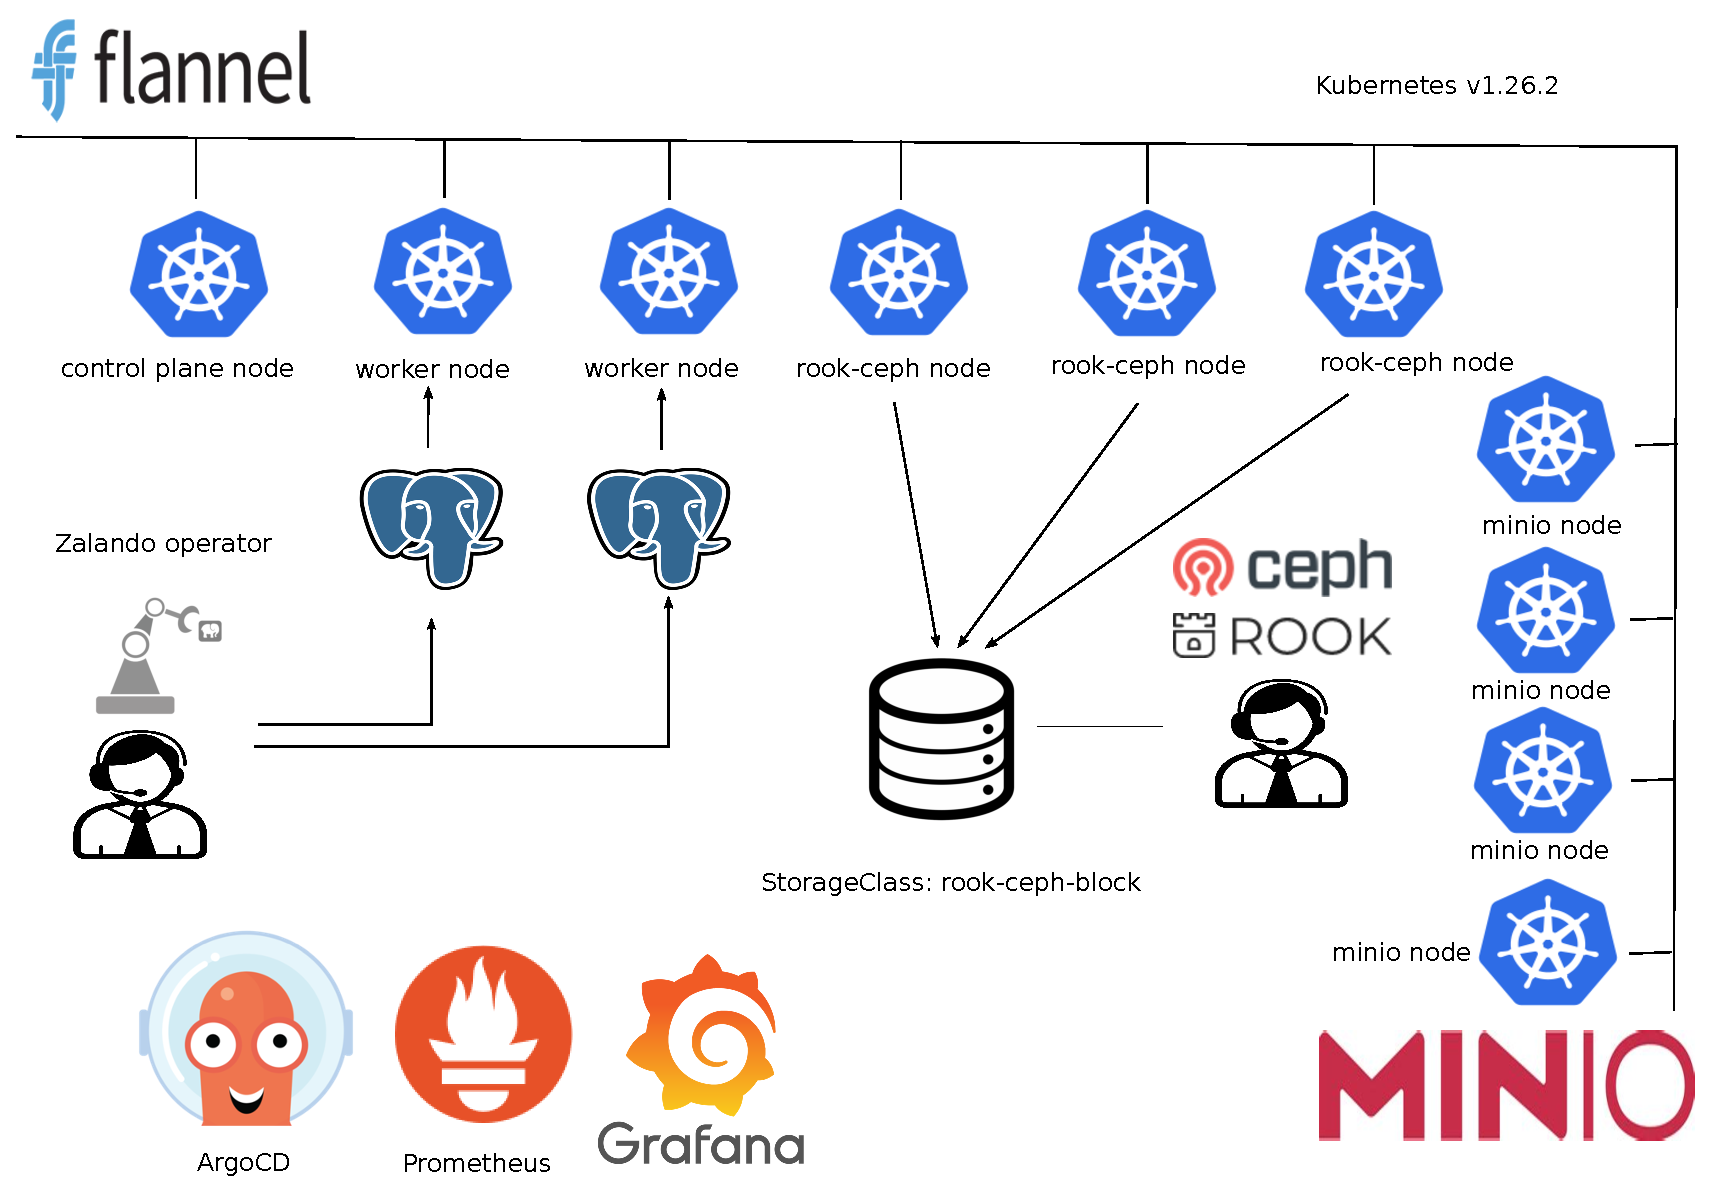
\includegraphics[scale=0.5]{images/architecture.eps}
\end{center}
\end{figure}

\end{frame}

%%%%%%%%%%%%%%%%%%%%%%%%%%%%%%%%%%%%%%%%%%%%%%%%%%%%%%%%%%%%%%%%%%%%%%%%%%%%%%%%

\begin{frame}[fragile]{Versions utilisées}

   \begin{itemize}
      \item OS de déploiement: Debian 11 - Bullseye
      \item Versions de Kubernetes: 1.26.x
   \end{itemize}

\end{frame}

%%%%%%%%%%%%%%%%%%%%%%%%%%%%%%%%%%%%%%%%%%%%%%%%%%%%%%%%%%%%%%%%%%%%%%%%%%%%%%%%

\begin{frame}[fragile]{Dimensionnement des serveurs}

   Dimensionnement du control plane:

   \begin{itemize}
      \item 8 CPU
      \item 8 Go RAM
   \end{itemize}

   Dimensionnement des workers:

   \begin{itemize}
      \item 2 CPU
      \item 2 Go RAM
   \end{itemize}

\end{frame}

%%%%%%%%%%%%%%%%%%%%%%%%%%%%%%%%%%%%%%%%%%%%%%%%%%%%%%%%%%%%%%%%%%%%%%%%%%%%%%%%

\begin{frame}[fragile]{Prérequis matériels}

   \begin{itemize}
      \item etcd est la base de données clé-valuers centrale utilisée par Kubernetes
      \item etcd utilise de manière intensive les disques à disposition
      \item Pour une stabilité accrue du cluster, il est préférable d'utiliser des disques de type \textbf{SSD}
   \end{itemize}

\end{frame}

%%%%%%%%%%%%%%%%%%%%%%%%%%%%%%%%%%%%%%%%%%%%%%%%%%%%%%%%%%%%%%%%%%%%%%%%%%%%%%%%

\begin{frame}[fragile]{Déploiement du n{\oe}ud \textbf{control plane}}

   \begin{itemize}
      \item Kubernetes s'appuie sur un élément essentiel qui est le \textit{container runtime}.
      \item La méthode de déploiement du container runtime s'appuie la méthode décrite dans le lien: \url{https://docs.docker.com/engine/install/debian/}
   \end{itemize}

\end{frame}

%%%%%%%%%%%%%%%%%%%%%%%%%%%%%%%%%%%%%%%%%%%%%%%%%%%%%%%%%%%%%%%%%%%%%%%%%%%%%%%%

\begin{frame}[fragile]{Désactivation permanente de la mémoire \textbf{swap}}

   Le process kubelet ne démarre pas en cas de mémoire swap activée.\\
   Pour désactiver l'utilisation de la swap, merci d'utiliser la commande suivante:
\begin{tiny}
\begin{Verbatim}[commandchars=\&\#\#]
swapoff -a
\end{Verbatim}
\end{tiny}

   Pour persister cet état et faire en sorte que la mémoire swap ne soit pas activée au prochain reboot, supprimer ou mettre en commentaires la ligne suivante dans \textit{/etc/fstab}:

\begin{tiny}
\begin{Verbatim}[commandchars=\\\{\}]
$ sudo cat /etc/fstab 
/dev/mapper/dnumworker1--vg-root /               ext4    errors=remount-ro 0       1
# /boot was on /dev/sda1 during installation
UUID=ddd6fd9d-6ac3-4510-9156-22984bc82b67 /boot           ext2    defaults        0       2
\textbf{#/dev/mapper/dnumworker1--vg-swap_1 none            swap    sw              0       0}
/dev/sr0        /media/cdrom0   udf,iso9660 user,noauto     0       0

\end{Verbatim}
\end{tiny}

\end{frame}

%%%%%%%%%%%%%%%%%%%%%%%%%%%%%%%%%%%%%%%%%%%%%%%%%%%%%%%%%%%%%%%%%%%%%%%%%%%%%%%%

\begin{frame}[fragile]{Installation du runtine container \textit{containerd}}

Mise à jour de l'index du paquet \textit{apt} et installation des paquets nécessaires à l'utilisation des dépôts avec le protocole HTTPS:

\begin{tiny}
\begin{Verbatim}[commandchars=\&\#\#]
sudo apt-get update

sudo apt-get install \
    ca-certificates \
    curl \
    gnupg

\end{Verbatim}
\end{tiny}

\end{frame}

%%%%%%%%%%%%%%%%%%%%%%%%%%%%%%%%%%%%%%%%%%%%%%%%%%%%%%%%%%%%%%%%%%%%%%%%%%%%%%%%

\begin{frame}[fragile]{Ajout de la clef GPG officielle de Docker}

\begin{tiny}
\begin{Verbatim}[commandchars=\&\#\#]
sudo install -m 0755 -d /etc/apt/keyrings
curl -fsSL https://download.docker.com/linux/debian/gpg | sudo gpg --dearmor -o /etc/apt/keyrings/docker.gpg
sudo chmod a+r /etc/apt/keyrings/docker.gpg
\end{Verbatim}
\end{tiny}

\end{frame}

%%%%%%%%%%%%%%%%%%%%%%%%%%%%%%%%%%%%%%%%%%%%%%%%%%%%%%%%%%%%%%%%%%%%%%%%%%%%%%%%

\begin{frame}[shrink=7,fragile]{Ajout du dépôt de Docker}

\begin{tiny}
\begin{Verbatim}[commandchars=\&\#\#]
  echo \
  "deb [arch="$(dpkg --print-architecture)" signed-by=/etc/apt/keyrings/docker.gpg] https://download.docker.com/linux/debian \
  "$(. /etc/os-release && echo "$VERSION_CODENAME")" stable" | \
  sudo tee /etc/apt/sources.list.d/docker.list > /dev/null
\end{Verbatim}
\end{tiny}

\end{frame}

%%%%%%%%%%%%%%%%%%%%%%%%%%%%%%%%%%%%%%%%%%%%%%%%%%%%%%%%%%%%%%%%%%%%%%%%%%%%%%%%

\begin{frame}[fragile]{Installation de Docker Engine}

\begin{tiny}
\begin{Verbatim}[commandchars=\&\#\#]
   sudo apt-get update
   sudo apt-get install docker-ce docker-ce-cli containerd.io docker-buildx-plugin docker-compose-plugin
\end{Verbatim}
\end{tiny}

\end{frame}

%%%%%%%%%%%%%%%%%%%%%%%%%%%%%%%%%%%%%%%%%%%%%%%%%%%%%%%%%%%%%%%%%%%%%%%%%%%%%%%%

\begin{frame}[fragile,shrink=0.9]{Installation de \textbf{kubectl, kubeadm et kubelet}}

\begin{tiny}
\begin{Verbatim}[commandchars=\&\#\#]
sudo apt-get install -y ca-certificates curl
sudo apt-get install -y apt-transport-https
sudo apt-get update
curl -fsSL https://packages.cloud.google.com/apt/doc/apt-key.gpg | sudo gpg --dearmor -o /etc/apt/keyrings/kubernetes-archive-keyring.gpg
echo "deb [signed-by=/etc/apt/keyrings/kubernetes-archive-keyring.gpg] \
https://apt.kubernetes.io/ kubernetes-xenial main" | \
sudo tee /etc/apt/sources.list.d/kubernetes.list

sudo apt-get update
sudo apt-get install -y kubectl
sudo apt-get install -y kubeadm
sudo apt-get install -y kubelet
\end{Verbatim}
\end{tiny}

\end{frame}

%%%%%%%%%%%%%%%%%%%%%%%%%%%%%%%%%%%%%%%%%%%%%%%%%%%%%%%%%%%%%%%%%%%%%%%%%%%%%%%%

\begin{frame}[fragile]{Activation des modules kernel \textit{overlay} et \textit{br\_netfilter}}

\begin{tiny}
\begin{Verbatim}[commandchars=\&\#\#]
linagora@debian-cp:/etc/modules-load.d$ cat k8s.conf 
overlay
br_netfilter
linagora@debian-cp:/etc/modules-load.d$ pwd
/etc/modules-load.d
\end{Verbatim}
\end{tiny}

\end{frame}

%%%%%%%%%%%%%%%%%%%%%%%%%%%%%%%%%%%%%%%%%%%%%%%%%%%%%%%%%%%%%%%%%%%%%%%%%%%%%%%%

\begin{frame}[fragile]{Activation des fonctions \textit{bridge/iptables} et \textit{forward} du kernel}

\begin{tiny}
\begin{Verbatim}[commandchars=\&\#\#]
linagora@debian-cp:/etc/sysctl.d$ cat k8s.conf 
inet.bridge.bridge-nf-call-iptables  = 1
net.bridge.bridge-nf-call-ip6tables = 1
net.ipv4.ip_forward                 = 1
linagora@debian-cp:/etc/sysctl.d$ pwd
/etc/sysctl.d
\end{Verbatim}
\end{tiny}

\end{frame}

%%%%%%%%%%%%%%%%%%%%%%%%%%%%%%%%%%%%%%%%%%%%%%%%%%%%%%%%%%%%%%%%%%%%%%%%%%%%%%%%

\begin{frame}[fragile]{Paramétrage de containerd}

Génération du paramétrage par défaut de containerd:

\begin{tiny}
\begin{Verbatim}[commandchars=\\\{\}]
root@debian-cp:~# containerd config \userinput{default} dump > /etc/containerd/config.toml.dmp
\end{Verbatim}
\end{tiny}

Modifier la valeur à \textbf{true} pour le paramètre \textbf{SystemdCgroup}:

\begin{tiny}
\begin{Verbatim}[commandchars=\\\{\}]
[plugins."io.containerd.grpc.v1.cri".containerd.runtimes.runc.options]
  BinaryName = ""
  CriuImagePath = ""
  CriuPath = ""
  CriuWorkPath = ""
  IoGid = 0
  IoUid = 0
  NoNewKeyring = false
  NoPivotRoot = false
  Root = ""
  ShimCgroup = ""
  SystemdCgroup = \userinput{true}
\end{Verbatim}
\end{tiny}

\end{frame}

%%%%%%%%%%%%%%%%%%%%%%%%%%%%%%%%%%%%%%%%%%%%%%%%%%%%%%%%%%%%%%%%%%%%%%%%%%%%%%%%

\begin{frame}[fragile]{Paramétrage de containerd}

Remplacer le paramétrage actuel par le paramétrage modifié:

\begin{tiny}
\begin{Verbatim}[commandchars=\\\{\}]
root@debian-cp:~# cp /etc/containerd/config.toml /etc/containerd/config.toml.bak
root@debian-cp:~# cat /etc/containerd/config.toml.dmp > /etc/containerd/config.toml
root@debian-cp:~# systemctl restart containerd
\end{Verbatim}
\end{tiny}

\end{frame}

%%%%%%%%%%%%%%%%%%%%%%%%%%%%%%%%%%%%%%%%%%%%%%%%%%%%%%%%%%%%%%%%%%%%%%%%%%%%%%%%

\begin{frame}[fragile]{Initialisation du cluster Kubernetes}

En tant que root, lancer la commande suivante:

\begin{tiny}
\begin{Verbatim}[commandchars=\&\@\@]
# kubeadm init --control-plane-endpoint 10.10.10.30 \
--skip-phases=addon/coredns,addon/kube-proxy \
--v=5 \
--pod-network-cidr="10.244.0.0/16"
\end{Verbatim}
\end{tiny}

Si les phases \textit{addon/coredns} et \textit{addon/kube-proxy} ne sont pas évitées au $1^{er}$ lancement de kubeadm, l'erreur suivante est générée:

\begin{tiny}
\begin{tcolorbox}
\lbrack kubelet-finalize\rbrack Updating "/etc/kubernetes/kubelet.conf" to point to a rotatable kubelet client certificate and key
error execution phase addon/coredns: unable to fetch CoreDNS current installed version and ConfigMap.: rpc error: code = Unknown desc = malformed header: missing HTTP content-type
To see the stack trace of this error execute with --v=5 or higher
\end{tcolorbox}
\end{tiny}

\end{frame}

%%%%%%%%%%%%%%%%%%%%%%%%%%%%%%%%%%%%%%%%%%%%%%%%%%%%%%%%%%%%%%%%%%%%%%%%%%%%%%%%

\begin{frame}[shrink=7,fragile]{Initialisation du cluster Kubernetes}

Le résultat de la commande d'init est le suivant:

\begin{tcolorbox}
I0315 01:06:38.342010   34405 kubeletfinalize.go:134\rbrack \lbrack kubelet-finalize\rbrack Restarting the kubelet to enable client certificate rotation\\
Your Kubernetes control-plane has initialized successfully!\\
To start using your cluster, you need to run the following as a regular user:

\begin{tiny}
\begin{Verbatim}[commandchars=\&\@\@]
  mkdir -p $HOME/.kube
  sudo cp -i /etc/kubernetes/admin.conf $HOME/.kube/config
  sudo chown $(id -u):$(id -g) $HOME/.kube/config
\end{Verbatim}
\end{tiny}

Alternatively, if you are the root user, you can run:\\

\begin{tiny}
\begin{Verbatim}[commandchars=\&\@\@]
  export KUBECONFIG=/etc/kubernetes/admin.conf
\end{Verbatim}
\end{tiny}

You should now deploy a pod network to the cluster.\\
Run "kubectl apply -f [podnetwork].yaml" with one of the options listed at:\\
  https://kubernetes.io/docs/concepts/cluster-administration/addons/

You can now join any number of control-plane nodes by copying certificate authorities
and service account keys on each node and then running the following as root:

\begin{tiny}
\begin{Verbatim}[commandchars=\&\@\@]
  kubeadm join 10.10.10.30:6443 --token 6pia7c.n6u8pbm7yjl6nnr8 \
        --discovery-token-ca-cert-hash sha256:f6d45602ea75c7659dc91f661d19e97e6817e2847e4e5d0047880b871317a145 \
        --control-plane 
\end{Verbatim}
\end{tiny}

Then you can join any number of worker nodes by running the following on each as root:

\begin{tiny}
\begin{Verbatim}[commandchars=\&\@\@]
kubeadm join 10.10.10.30:6443 --token 6pia7c.n6u8pbm7yjl6nnr8 \
        --discovery-token-ca-cert-hash sha256:f6d45602ea75c7659dc91f661d19e97e6817e2847e4e5d0047880b871317a145 
\end{Verbatim}
\end{tiny}
\end{tcolorbox}

\end{frame}

%%%%%%%%%%%%%%%%%%%%%%%%%%%%%%%%%%%%%%%%%%%%%%%%%%%%%%%%%%%%%%%%%%%%%%%%%%%%%%%%

\begin{frame}[fragile]{Paramétrage de \textit{kubectl}}

   L'utilisation de kubectl nécessite l'action suivante:

\begin{tiny}
\begin{Verbatim}[commandchars=\&\@\@]
  mkdir -p $HOME/.kube
  sudo cp -i /etc/kubernetes/admin.conf $HOME/.kube/config
  sudo chown $(id -u):$(id -g) $HOME/.kube/config
\end{Verbatim}
\end{tiny}

\end{frame}

%%%%%%%%%%%%%%%%%%%%%%%%%%%%%%%%%%%%%%%%%%%%%%%%%%%%%%%%%%%%%%%%%%%%%%%%%%%%%%%%

\begin{frame}[fragile]{Déploiement de l'addon \textbf{CoreDNS}}

   Comme indiqué précédemment, les addons CoreDNS et Kube-Proxy n'ont pas été déployés au $1^{er}$ lancement de kubeadm.\\
   CoreDNS peut maintenant être déployé sans erreur:\\

\begin{tiny}
\begin{Verbatim}[commandchars=\\\{\}]
linagora@debian-cp:~$ sudo kubeadm init phase addon coredns
[addons] Applied essential addon: CoreDNS
\end{Verbatim}
\end{tiny}

\end{frame}

%%%%%%%%%%%%%%%%%%%%%%%%%%%%%%%%%%%%%%%%%%%%%%%%%%%%%%%%%%%%%%%%%%%%%%%%%%%%%%%%

\begin{frame}[fragile]{Déploiement de l'addon \textbf{Kube-Proxy}}

\begin{tiny}
\begin{Verbatim}[commandchars=\\\{\}]
linagora@debian-cp:~$ sudo kubeadm init phase addon kube-proxy
[addons] Applied essential addon: kube-proxy
\end{Verbatim}
\end{tiny}

\end{frame}

%%%%%%%%%%%%%%%%%%%%%%%%%%%%%%%%%%%%%%%%%%%%%%%%%%%%%%%%%%%%%%%%%%%%%%%%%%%%%%%%

\begin{frame}[fragile]{Choix de la couche réseau - \textbf{Container Network Interface}}

   Il existe différentes addons Kubernetes implémentant l'interface CNI.\\
   Ces addons sont listés dans l'URL suivante: \url{https://kubernetes.io/docs/concepts/cluster-administration/addons/}\\
   Pour le POC, l'addon sélectionné est Flannel car il semble être le plus simple et le plus basique des addons CNI.\\

\end{frame}

%%%%%%%%%%%%%%%%%%%%%%%%%%%%%%%%%%%%%%%%%%%%%%%%%%%%%%%%%%%%%%%%%%%%%%%%%%%%%%%%

\begin{frame}[fragile]{Déploiement de l'addon \textit{Flannel}}

   L'addon Flannel s'installe de plusieurs manières (\url{https://github.com/flannel-io/flannel#deploying-flannel-manually}).\\
   La méthode utilisée pour le POC est kubectl:

\begin{tiny}
\begin{Verbatim}[commandchars=\\\{\}]
kubectl apply -f https://github.com/flannel-io/flannel/releases/latest/download/kube-flannel.yml
\end{Verbatim}
\end{tiny}

\end{frame}

%%%%%%%%%%%%%%%%%%%%%%%%%%%%%%%%%%%%%%%%%%%%%%%%%%%%%%%%%%%%%%%%%%%%%%%%%%%%%%%%

\begin{frame}[fragile]{Installation de \textbf{k9s}}

   Un outil pratique de visualisation d'un cluster kubernetes est: \textbf{k9s} (\url{https://k9scli.io/})\\
   Le lien suivant permet de télécharger l'archive incluant le binaire: \url{https://github.com/derailed/k9s/releases/download/v0.27.3/k9s_Linux_amd64.tar.gz}


\end{frame}

%%%%%%%%%%%%%%%%%%%%%%%%%%%%%%%%%%%%%%%%%%%%%%%%%%%%%%%%%%%%%%%%%%%%%%%%%%%%%%%%

\begin{frame}[fragile]{Liste des namespaces}

\begin{tiny}
\begin{Verbatim}[commandchars=\\\{\}]
linagora@debian-cp:~$ kubectl get namespaces
NAME              STATUS   AGE
default           Active   40d
kube-flannel      Active   39d
kube-node-lease   Active   40d
kube-public       Active   40d
kube-system       Active   40d
minio-operator    Active   32d
rook-ceph         Active   32d
\end{Verbatim}
\end{tiny}

\begin{figure}
\begin{center}
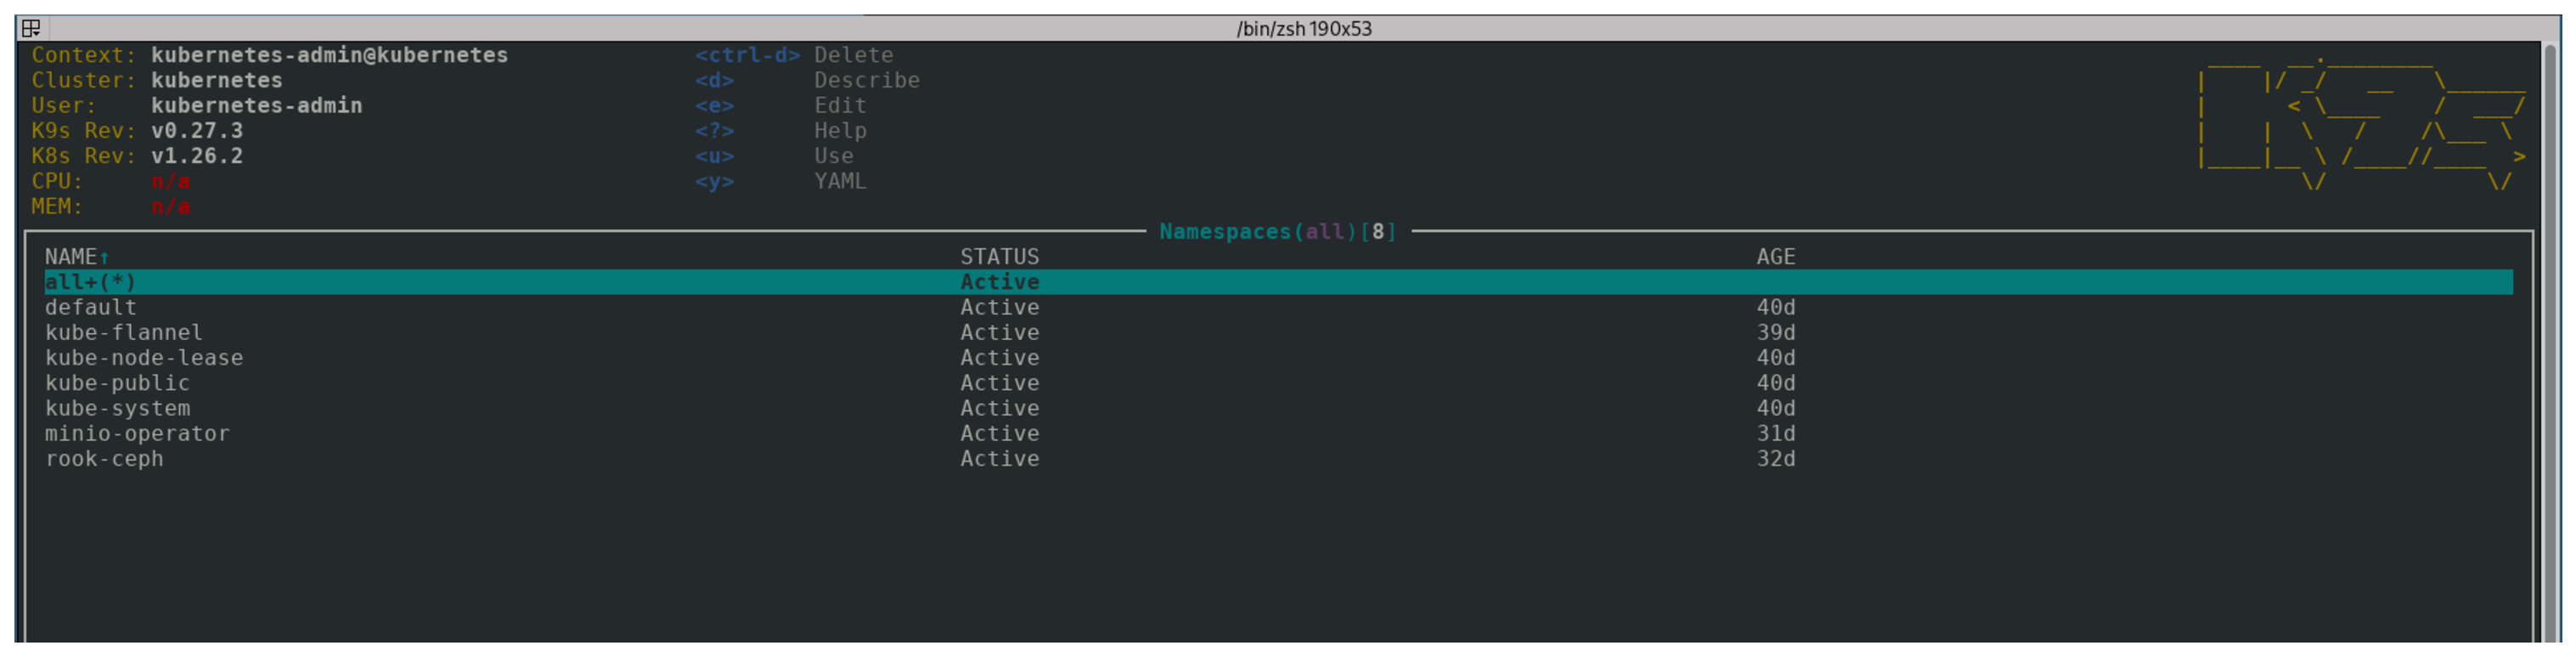
\includegraphics[angle=0, width=0.5\textwidth]{namespaces.eps}
\end{center}
\end{figure}

\end{frame}

%%%%%%%%%%%%%%%%%%%%%%%%%%%%%%%%%%%%%%%%%%%%%%%%%%%%%%%%%%%%%%%%%%%%%%%%%%%%%%%%

\begin{frame}[fragile]{Pods du namespace default}

\begin{tiny}
\begin{Verbatim}[commandchars=\\\{\}]
linagora@debian-cp:~$ kubectl get pods          
NAME                                    READY   STATUS    RESTARTS   AGE
acid-test-cluster-0                     1/1     Running   0          27d
acid-test-cluster-1                     1/1     Running   0          27d
postgres-operator-fcbd7cc96-ndpj8       1/1     Running   0          40d
postgres-operator-ui-5579cc7779-86rqk   1/1     Running   0          40d
\end{Verbatim}
\end{tiny}

\begin{figure}
\begin{center}
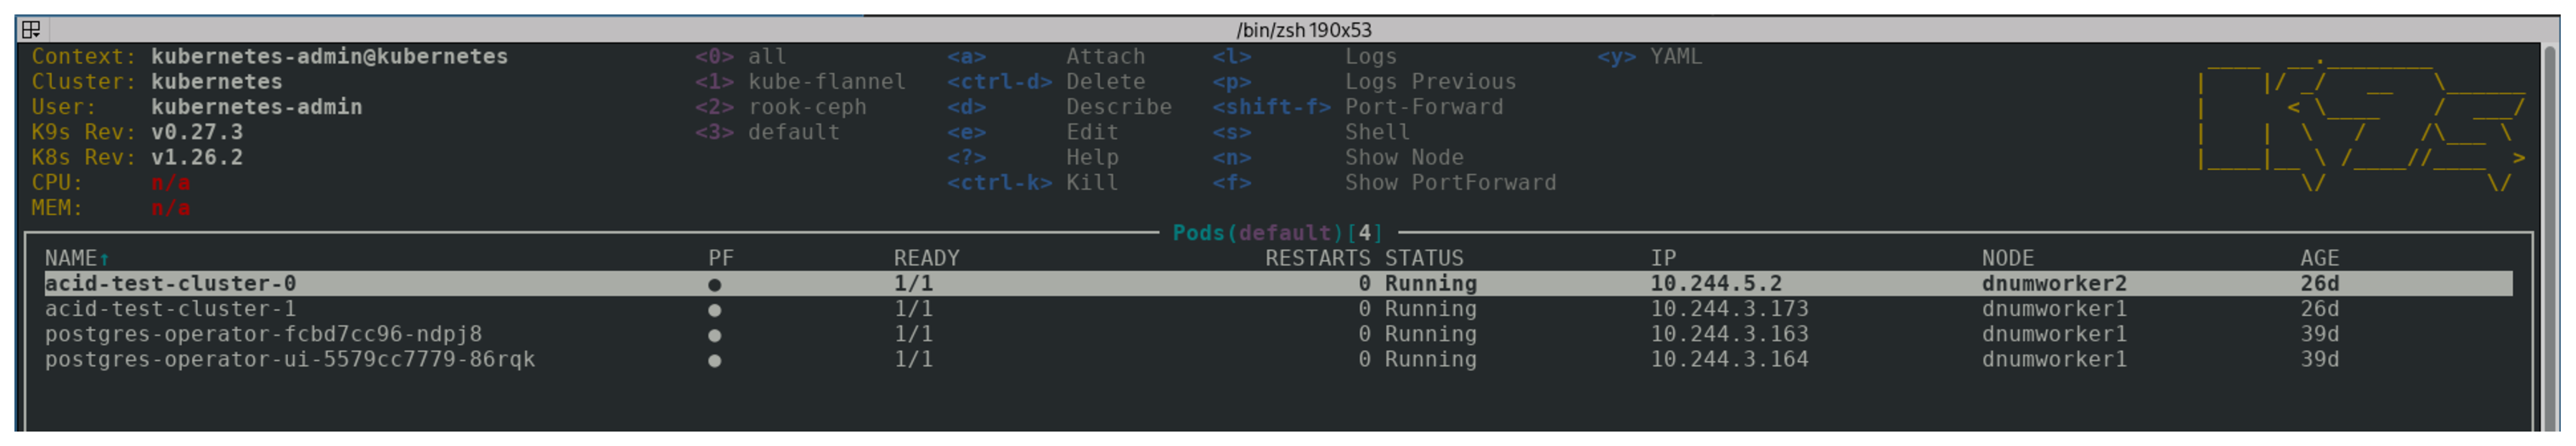
\includegraphics[angle=0, width=0.5\textwidth]{pod-default-ns.eps}
\end{center}
\end{figure}

\end{frame}

%%%%%%%%%%%%%%%%%%%%%%%%%%%%%%%%%%%%%%%%%%%%%%%%%%%%%%%%%%%%%%%%%%%%%%%%%%%%%%%%

\begin{frame}[fragile]{Pods du namespace kube-system}

\begin{tiny}
\begin{Verbatim}[commandchars=\\\{\}]
linagora@debian-cp:~$ kubectl get pods -n kube-system
NAME                                READY   STATUS    RESTARTS           AGE
coredns-787d4945fb-8ph9v            1/1     Running   0                  40d
coredns-787d4945fb-9jrzs            1/1     Running   0                  40d
etcd-debian-cp                      1/1     Running   158                41d
kube-apiserver-debian-cp            0/1     Running   4968 (13m ago)     41d
kube-controller-manager-debian-cp   1/1     Running   4161 (8m26s ago)   41d
kube-proxy-4mfn8                    1/1     Running   0                  33d
kube-proxy-9h4c6                    1/1     Running   0                  27d
kube-proxy-9j47t                    1/1     Running   0                  33d
kube-proxy-s78vx                    1/1     Running   0                  33d
kube-proxy-wpwt4                    1/1     Running   0                  40d
kube-proxy-xjs5q                    1/1     Running   1 (33d ago)        41d
kube-scheduler-debian-cp            1/1     Running   2848 (6m20s ago)   41d
\end{Verbatim}
\end{tiny}

\begin{figure}
\begin{center}
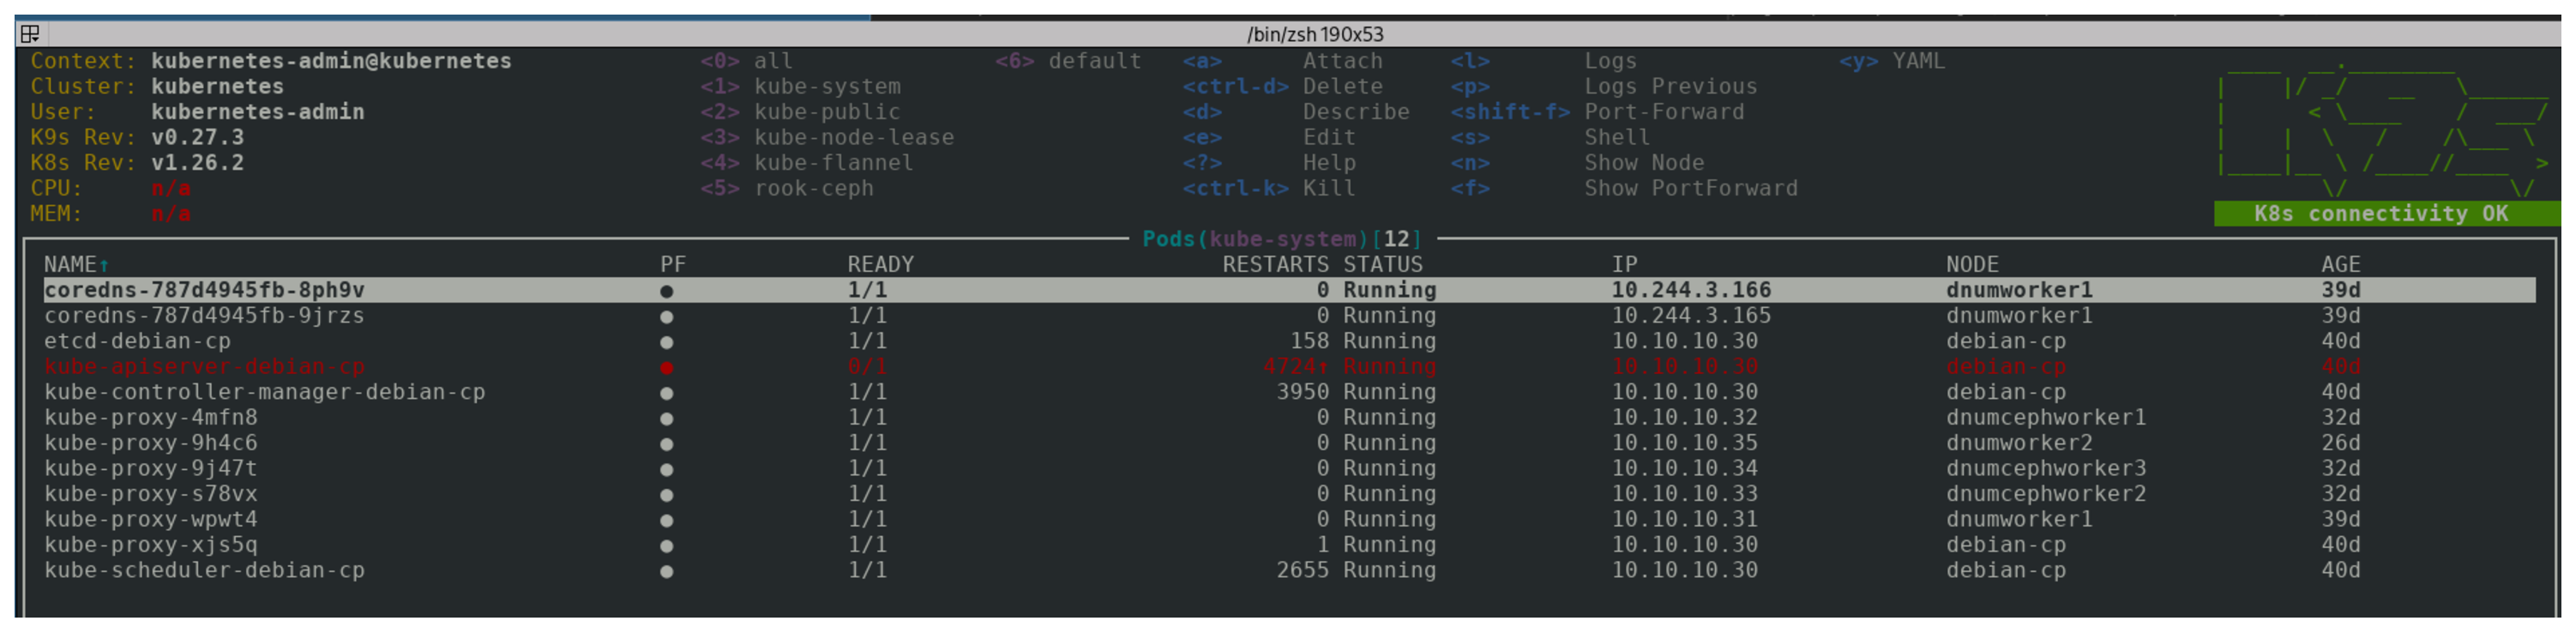
\includegraphics[angle=0, width=0.5\textwidth]{pod-kube-system.eps}
\end{center}
\end{figure}

\end{frame}

%%%%%%%%%%%%%%%%%%%%%%%%%%%%%%%%%%%%%%%%%%%%%%%%%%%%%%%%%%%%%%%%%%%%%%%%%%%%%%%%

\begin{frame}[fragile]{Pods du namespace kube-flannel}

\begin{tiny}
\begin{Verbatim}[commandchars=\\\{\}]
linagora@debian-cp:~$ kubectl get pods -n kube-flannel                                                                                                                                        
NAME                    READY   STATUS    RESTARTS      AGE                                                                                                                                   
kube-flannel-ds-5nw2j   1/1     Running   0             33d                                                                                                                                   
kube-flannel-ds-5xwsm   1/1     Running   0             40d                                                                                                                                   
kube-flannel-ds-8vkg9   1/1     Running   1 (33d ago)   40d                                                                                                                                   
kube-flannel-ds-pv6ss   1/1     Running   0             27d                                                                                                                                   
kube-flannel-ds-trbz9   1/1     Running   0             33d                                                                                                                                   
kube-flannel-ds-wmzz2   1/1     Running   0             33d
\end{Verbatim}
\end{tiny}

\begin{figure}
\begin{center}
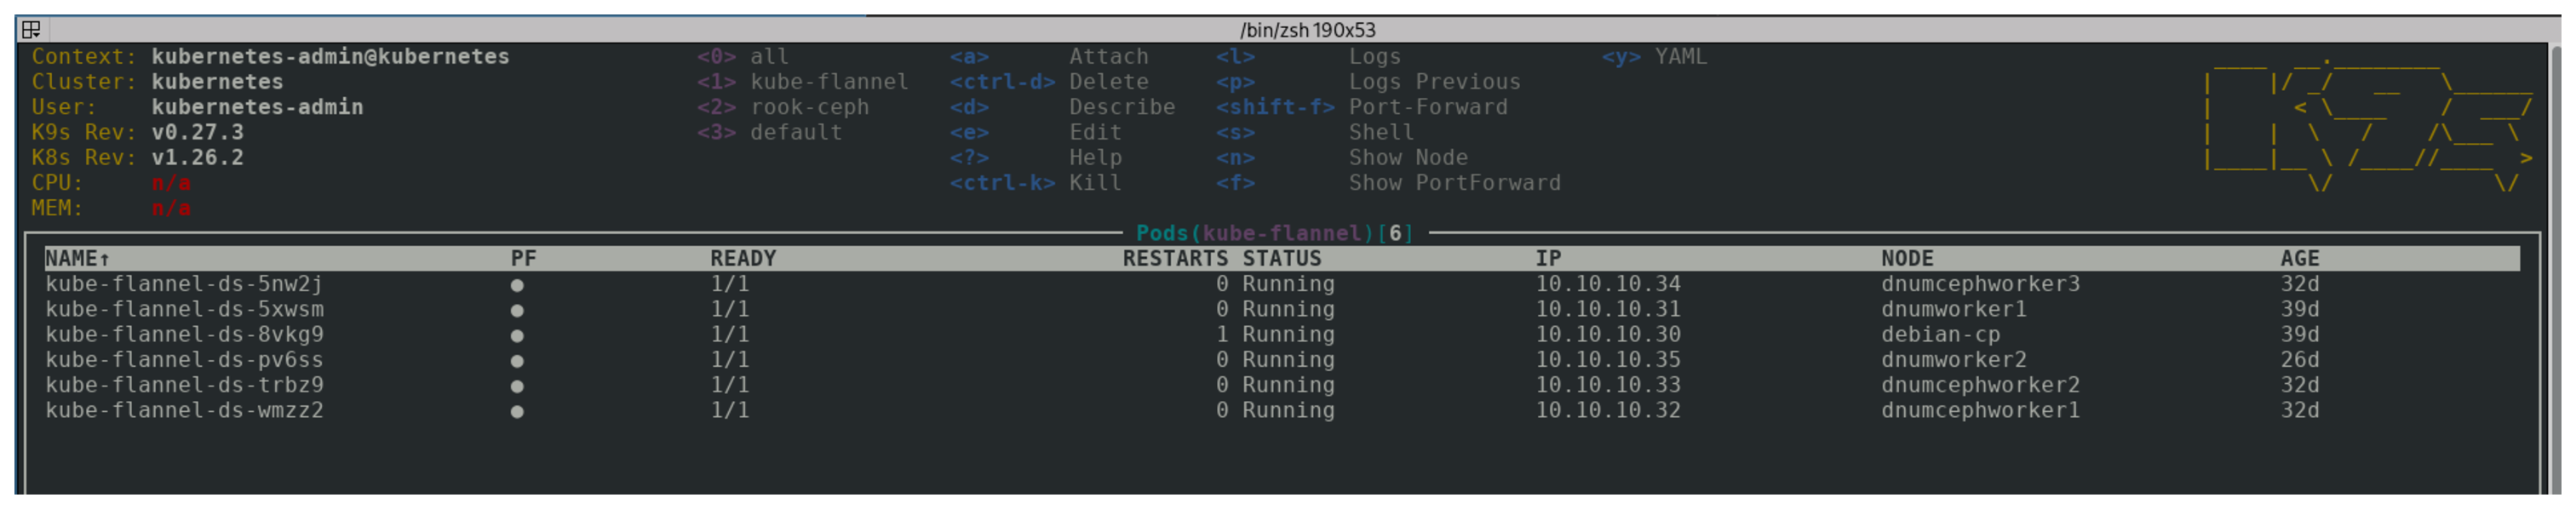
\includegraphics[angle=0, width=0.5\textwidth]{flannel.eps}
\end{center}
\end{figure}

\end{frame}

%%%%%%%%%%%%%%%%%%%%%%%%%%%%%%%%%%%%%%%%%%%%%%%%%%%%%%%%%%%%%%%%%%%%%%%%%%%%%%%%

\begin{frame}[fragile,shrink=0.9]{Pods du namespace rook-ceph}

\begin{tiny}
\begin{Verbatim}[commandchars=\\\{\}]
linagora@debian-cp:~$ kubectl get pods -n rook-ceph
NAME                                                        READY   STATUS                 RESTARTS           AGE
csi-cephfsplugin-9nbts                                      2/2     Running                1 (27d ago)        27d
csi-cephfsplugin-bpxlw                                      2/2     Running                0                  33d
csi-cephfsplugin-jd5x8                                      2/2     Running                0                  33d
csi-cephfsplugin-mddkf                                      2/2     Running                0                  33d
csi-cephfsplugin-nrmfz                                      2/2     Running                0                  33d
csi-cephfsplugin-provisioner-84cc595b78-9mml4               5/5     Running                6008 (2m44s ago)   33d
csi-cephfsplugin-provisioner-84cc595b78-9twnq               5/5     Running                2171               33d
csi-rbdplugin-92zlq                                         2/2     Running                0                  33d
csi-rbdplugin-c95w7                                         2/2     Running                0                  33d
csi-rbdplugin-pk57s                                         2/2     Running                1 (27d ago)        27d
csi-rbdplugin-provisioner-6f6b6b8cd6-4c8jd                  1/5     CreateContainerError   1344               33d
csi-rbdplugin-provisioner-6f6b6b8cd6-gw6bm                  1/5     CreateContainerError   4465               33d
csi-rbdplugin-srtfz                                         2/2     Running                0                  33d
csi-rbdplugin-v6gqm                                         2/2     Running                0                  33d
rook-ceph-crashcollector-dnumcephworker1-7845bb8ff-vs9fx    1/1     Running                0                  32d
rook-ceph-crashcollector-dnumcephworker2-75cdf95dcd-n5xsz   1/1     Running                0                  33d
rook-ceph-crashcollector-dnumcephworker3-6fddb6cd9-x45w5    1/1     Running                1 (8d ago)         32d
rook-ceph-mgr-a-c5db58dff-hvsp9                             3/3     Running                1487 (6d6h ago)    33d
rook-ceph-mgr-b-7bbfd88c8b-wh4ww                            2/3     CreateContainerError   944                22d
rook-ceph-mon-a-75cf9ccddc-b2jgc                            2/2     Running                1163               33d
rook-ceph-mon-b-78d6586d5-qss4z                             1/2     CreateContainerError   701 (19d ago)      19d
rook-ceph-mon-c-64dcb4c86c-wz8sg                            2/2     Running                1755               33d
rook-ceph-operator-cf4f7dfd4-6tm6p                          1/1     Running                0                  32d
rook-ceph-osd-0-57d9b8db4d-d6dhr                            1/2     CreateContainerError   484                32d
rook-ceph-osd-1-74698f77fd-6n2mh                            1/2     Running                529                32d
rook-ceph-osd-2-5cc486467c-lhm47                            1/2     Running                1116 (49m ago)     32d
rook-ceph-osd-prepare-dnumcephworker1-rnk78                 0/1     Completed              0                  21d
rook-ceph-osd-prepare-dnumcephworker3-42rxv                 0/1     Completed              0                  21d
rook-ceph-tools-7c4b8bb9b5-pxk67                            1/1     Running                0                  33d
\end{Verbatim}
\end{tiny}

\begin{figure}
\begin{center}
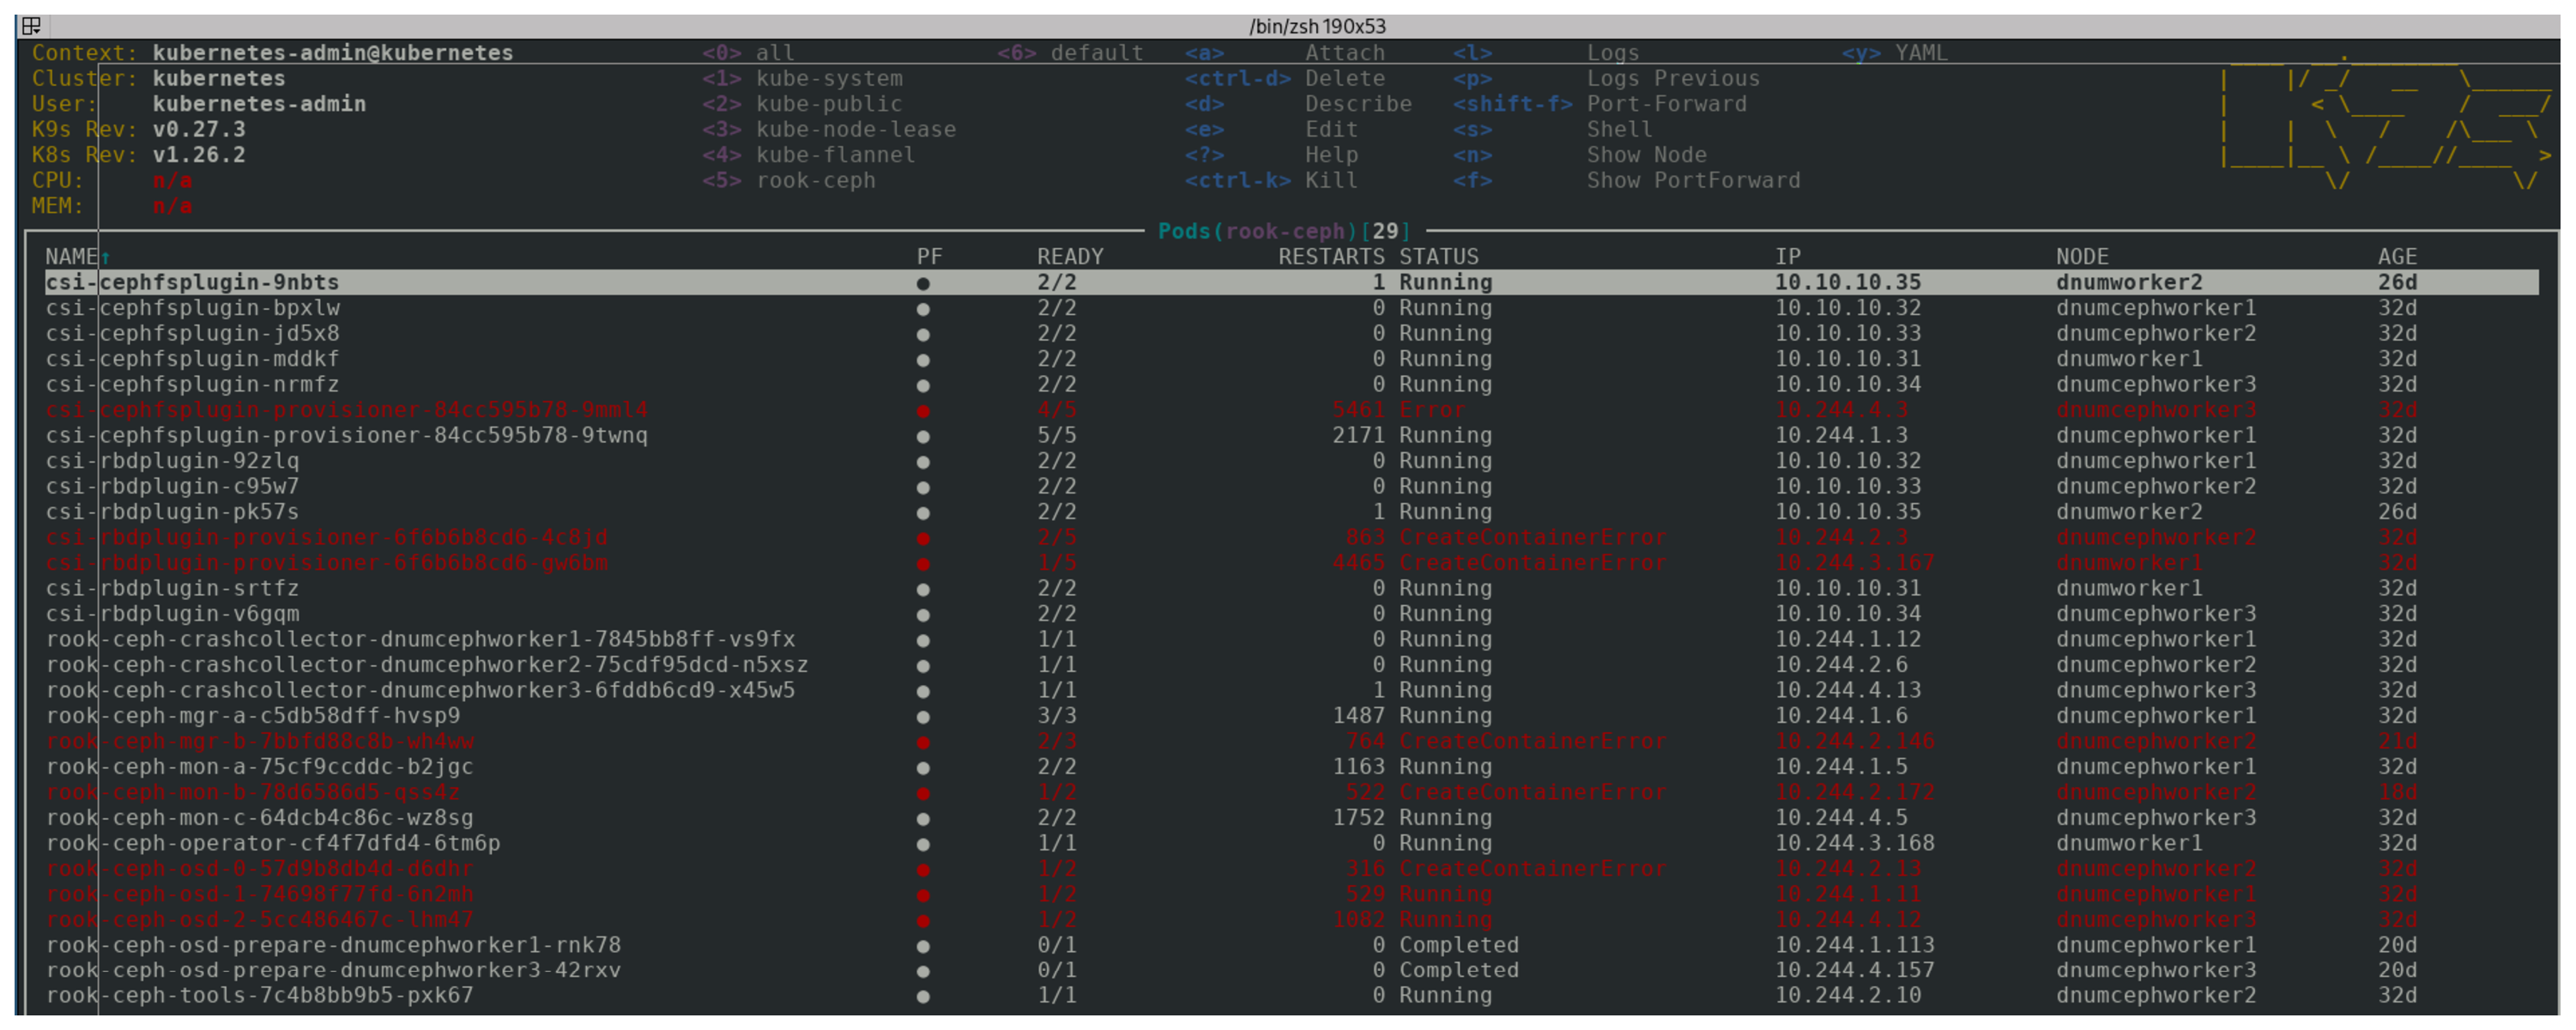
\includegraphics[angle=0, width=0.5\textwidth]{pod-rook-ceph.eps}
\end{center}
\end{figure}

\end{frame}

%%%%%%%%%%%%%%%%%%%%%%%%%%%%%%%%%%%%%%%%%%%%%%%%%%%%%%%%%%%%%%%%%%%%%%%%%%%%%%%%

\begin{frame}[fragile]{Déploiement du n{\oe}ud \textbf{worker}}

   Sur chacun des 2 workers, il est nécessaire de déployer:
   \begin{itemize}
      \item le runtime containerd de Docker
      \item les commandes kubectl, kubeadm et kubelet
      \item l'activation des modules kernel overlay et br\_netfilter
      \item l'activation des fonctions bridge/iptables et forward du kernel
      \item le paramétrage de containerd
   \end{itemize}

\end{frame}

%%%%%%%%%%%%%%%%%%%%%%%%%%%%%%%%%%%%%%%%%%%%%%%%%%%%%%%%%%%%%%%%%%%%%%%%%%%%%%%%

\begin{frame}[shrink=8,fragile]{Ajout du n{\oe}ud \textbf{worker} dans le cluster k8s - \textbf{join}}

   L'opération qui permet au n{\oe}ud worker de rejoindre le cluster s'appelle le join.\\
   La syntaxe de cette commande est obtenue en lançant la commande suivante sur le control plane avec l'utilisateur root:

\begin{tiny}
\begin{Verbatim}[commandchars=\&\@\@]
# kubeadm token create --print-join-command
kubeadm join 10.10.10.30:6443 \
--token ilfbgc.8xco4svm5pnxkfbj \
--discovery-token-ca-cert-hash sha256:73bf45619ae0051d4ff810328d1dadc18e6a5966c95d3c4ec76275b89a934595 
\end{Verbatim}
\end{tiny}

\end{frame}

%%%%%%%%%%%%%%%%%%%%%%%%%%%%%%%%%%%%%%%%%%%%%%%%%%%%%%%%%%%%%%%%%%%%%%%%%%%%%%%%

\begin{frame}[fragile]{Lancement du join sur chacun des workers}

Sur chacun des workers, le lancement de la commande join produit le résultat suivant:
\begin{tcolorbox}
\begin{tiny}
\begin{Verbatim}[commandchars=\&\@\@]
# kubeadm join 10.10.10.30:6443 \
--token 6pia7c.n6u8pbm7yjl6nnr8 \
--discovery-token-ca-cert-hash sha256:f6d45602ea75c7659dc91f661d19e97e6817e2847e4e5d0047880b871317a145
[preflight] Running pre-flight checks
[preflight] Reading configuration from the cluster...
[preflight] FYI: You can look at this config file with 'kubectl -n kube-system \
get cm kubeadm-config -o yaml'
W0315 16:31:41.445771 6266 configset.go:78] Warning: No kubeproxy.config.k8s.io/v1alpha1 config is loaded.
Continuing without it: configmaps "kube-proxy" is forbidden: User "system:bootstrap:6pia7c"
cannot get resource "configmaps" in API group "" in the namespace "kube-system"
[kubelet-start] Writing kubelet configuration to file "/var/lib/kubelet/config.yaml"
[kubelet-start] Writing kubelet environment file with flags to file "/var/lib/kubelet/kubeadm-flags.env"
[kubelet-start] Starting the kubelet
[kubelet-start] Waiting for the kubelet to perform the TLS Bootstrap...

This node has joined the cluster:
* Certificate signing request was sent to apiserver and a response was received.
* The Kubelet was informed of the new secure connection details.

Run 'kubectl get nodes' on the control-plane to see this node join the cluster.
\end{Verbatim}
\end{tiny}
\end{tcolorbox}

\end{frame}

%%%%%%%%%%%%%%%%%%%%%%%%%%%%%%%%%%%%%%%%%%%%%%%%%%%%%%%%%%%%%%%%%%%%%%%%%%%%%%%%

\begin{frame}[fragile]{Lancement du join sur chacun des workers}

La commande suivante permet de vérifier le résultat du join:
\begin{tiny}
\begin{Verbatim}[commandchars=\&\@\@]
$ kubectl get nodes
NAME          STATUS     ROLES           AGE   VERSION
debian-cp     NotReady   control-plane   15h   v1.26.2
dnumworker1   NotReady   <none>          53s   v1.26.2

\end{Verbatim}
\end{tiny}

\end{frame}

%%%%%%%%%%%%%%%%%%%%%%%%%%%%%%%%%%%%%%%%%%%%%%%%%%%%%%%%%%%%%%%%%%%%%%%%%%%%%%%%

\begin{frame}[shrink=8,fragile]{Terminologie du stockage dans k8s}

\begin{itemize}
   \item Le stockage permanent des données s'appuie les volumes persistants (PV) (\url{https://kubernetes.io/docs/concepts/storage/persistent-volumes/})
   \item Un PV est un espace de stockage mis à disposition par k8s.
   \item Il peut être alloué manuellement ou dynamiquement par l'intermédiaire des storage class (\url{https://kubernetes.io/docs/concepts/storage/storage-classes/})
   \item Les PV sont l'équivalent d'un node dans un cluster.
   \item Les persistentVolumeClaim (PVC) sont l'équivalent d'un pod.
\end{itemize}

\end{frame}

%%%%%%%%%%%%%%%%%%%%%%%%%%%%%%%%%%%%%%%%%%%%%%%%%%%%%%%%%%%%%%%%%%%%%%%%%%%%%%%%

\begin{frame}[fragile]{Déploiement du stockage - \textbf{Rook Ceph}}

\begin{itemize}
   \item Le storage class sur lequel s'appuie l'opérateur PostgreSQL est Ceph
   \item L'opérateur k8s \textbf{Rook Ceph} facilite le déploiement de Ceph
   \item Le déploiement s'appuie sur le lien \url{https://rook.io/docs/rook/v1.9/quickstart.html}
   \item La version de l'opérateur utilisée est la v1.9
   \item Elle supporte les versions k8s v1.17+
\end{itemize}

\end{frame}

%%%%%%%%%%%%%%%%%%%%%%%%%%%%%%%%%%%%%%%%%%%%%%%%%%%%%%%%%%%%%%%%%%%%%%%%%%%%%%%%

\begin{frame}[fragile]{Prérequis au déploiement de l'opérateur - \textbf{Rook Ceph}}

\begin{itemize}
   \item Le déploiement de l'opérateur scanne l'ensemble des noeuds de stockage pour vérifier la présence de:
   \begin{itemize}
      \item des devices bruts (sans partitions ou filesystems formattés)
      \item des partitions brutes (sans filesystems formattés)
      \item les volumes physiques initialisés par LVM
   \end{itemize}
\end{itemize}

L'exemple ci-dessous indique comment vérifier la disponibilité d'espace pour l'opérateur Rook Ceph:

\begin{tiny}
\begin{Verbatim}[commandchars=\\\{\}]
lsblk -f

    NAME                  FSTYPE      LABEL UUID                                   MOUNTPOINT
    vda
    |-vda1                LVM2_member       >eSO50t-GkUV-YKTH-WsGq-hNJY-eKNf-3i07IB
     |-ubuntu--vg-root   ext4              c2366f76-6e21-4f10-a8f3-6776212e2fe4   /
     |-ubuntu--vg-swap_1 swap              9492a3dc-ad75-47cd-9596-678e8cf17ff9   [SWAP]
    vdb
\end{Verbatim}
\end{tiny}

\end{frame}

%%%%%%%%%%%%%%%%%%%%%%%%%%%%%%%%%%%%%%%%%%%%%%%%%%%%%%%%%%%%%%%%%%%%%%%%%%%%%%%%

\begin{frame}[fragile]{Prérequis au déploiement de l'opérateur - \textbf{Rook Ceph}}

\begin{itemize}
   \item Dans l'exemple précédent, si la colonne \textit{FSTYPE} est renseignée, cela indique la présence d'un filesystem
   \item La partition vdb n'est pas formatée avec un filesystem: elle est donc utilisable par l'opérateur Rook Ceph
   \item Le paquet \textbf{lvm2} est une dépendance importante de Rook Ceph
\end{itemize}

\end{frame}

%%%%%%%%%%%%%%%%%%%%%%%%%%%%%%%%%%%%%%%%%%%%%%%%%%%%%%%%%%%%%%%%%%%%%%%%%%%%%%%%

\begin{frame}[fragile]{Sélection des n\oe{}uds sur lesquels \textbf{Ceph} sera déployé}

   L'opérateur Rook Ceph offre la possibilité de sélectionner les n\oe{}uds sur lesquels le stockage Ceph est déployé.\\
   Pour cela, il s'appuie sur la notion de label.\\
   Dans le cadre du POC, les 3 n\oe{}uds suivants sont sélectionnés pour porter le stockage:
\begin{itemize}
   \item dnumcephworker1
   \item dnumcephworker2
   \item dnumcephworker3
\end{itemize}

\end{frame}

%%%%%%%%%%%%%%%%%%%%%%%%%%%%%%%%%%%%%%%%%%%%%%%%%%%%%%%%%%%%%%%%%%%%%%%%%%%%%%%%

\begin{frame}[shrink=7,fragile]{Affectation des labels sur les n\oe{}uds de stockage}

   Depuis le control plane, lancer les commandes suivantes pour marquer les n\oe{}uds:
\begin{tiny}
\begin{Verbatim}[commandchars=\\\{\}]
$ kubectl label nodes dnumcephworker1 role=storage-node
node/dnumcephworker1 labeled
$ kubectl label nodes dnumcephworker2 role=storage-node
node/dnumcephworker2 labeled
$ kubectl label nodes dnumcephworker3 role=storage-node
node/dnumcephworker3 labeled
\end{Verbatim}
\end{tiny}

   Affichage du label des n\oe{}uds:
\begin{tiny}
\begin{Verbatim}[commandchars=\\\{\}]
$ kubectl get nodes --show-labels
NAME              STATUS   ROLES           LABELS
dnumcephworker1   Ready    <none>          kubernetes.io/hostname=dnumcephworker1,kubernetes.io/os=linux,\textbf{role=storage-node}
dnumcephworker2   Ready    <none>          kubernetes.io/hostname=dnumcephworker2,kubernetes.io/os=linux,\textbf{role=storage-node}
dnumcephworker3   Ready    <none>          kubernetes.io/hostname=dnumcephworker3,kubernetes.io/os=linux,\textbf{role=storage-node}
\end{Verbatim}
\end{tiny}
\end{frame}

%%%%%%%%%%%%%%%%%%%%%%%%%%%%%%%%%%%%%%%%%%%%%%%%%%%%%%%%%%%%%%%%%%%%%%%%%%%%%%%%

\begin{frame}[shrink=5,fragile]{Paramétrage pour la répartition du stockage Ceph sur les n\oe{}uds labelisés}

\begin{tiny}
\begin{Verbatim}[commandchars=\\\{\}]
~/rook$ git diff
diff --git a/deploy/examples/cluster.yaml b/deploy/examples/cluster.yaml
index 9bd50ec97..fef3f777f 100644
--- a/deploy/examples/cluster.yaml
+++ b/deploy/examples/cluster.yaml
@@ -154,22 +154,22 @@ spec:
   # To control where various services will be scheduled by kubernetes, use the placement configuration sections below.
   # The example under 'all' would have all services scheduled on kubernetes nodes labeled with 'role=storage-node' and
   # tolerate taints with a key of 'storage-node'.
-  # placement:
-  #   all:
-  #     nodeAffinity:
-  #       requiredDuringSchedulingIgnoredDuringExecution:
-  #         nodeSelectorTerms:
-  #         - matchExpressions:
-  #           - key: role
-  #             operator: In
-  #             values:
-  #             - storage-node
-  #     podAffinity:
-  #     podAntiAffinity:
-  #     topologySpreadConstraints:
-  #     tolerations:
-  #     - key: storage-node
-  #       operator: Exists
+  placement:
+    all:
+      nodeAffinity:
+        requiredDuringSchedulingIgnoredDuringExecution:
+          nodeSelectorTerms:
+          - matchExpressions:
+            - key: role
+              operator: In
+              values:
\textbf{+              - storage-node}
+      podAffinity:
+      podAntiAffinity:
+      topologySpreadConstraints:
+      tolerations:
+      - key: storage-node
+        operator: Exists
   # The above placement information can also be specified for mon, osd, and mgr components
   #   mon:
   # Monitor deployments may contain an anti-affinity rule for avoiding monitor
\end{Verbatim}
\end{tiny}


\end{frame}

%%%%%%%%%%%%%%%%%%%%%%%%%%%%%%%%%%%%%%%%%%%%%%%%%%%%%%%%%%%%%%%%%%%%%%%%%%%%%%%%

\begin{frame}[fragile]{Paramétrage pour la répartition du stockage Ceph sur les n\oe{}uds labelisés}

   La directive \textit{nodeSelectorTerms} permet de sélectionner les noeuds portant la storageclass Ceph

\begin{tiny}
\begin{Verbatim}[commandchars=\\\{\}]
+          nodeSelectorTerms:
\ldots
\textbf{+              - storage-node}
+      podAffinity:
+      podAntiAffinity:
\end{Verbatim}
\end{tiny}


\end{frame}

%%%%%%%%%%%%%%%%%%%%%%%%%%%%%%%%%%%%%%%%%%%%%%%%%%%%%%%%%%%%%%%%%%%%%%%%%%%%%%%%

\begin{frame}[fragile]{Déploiement de l'opérateur \textbf{Rook Ceph}}

   Comme indiqué dans le lien \url{https://rook.io/docs/rook/v1.9/quickstart.html}, l'application des commandes ci-dessous amorce le déploiement de l'opérateur:

\begin{tiny}
\begin{Verbatim}[commandchars=\\\{\}]
$ git clone --single-branch --branch v1.9.2 https://github.com/rook/rook.git
cd rook/deploy/examples
kubectl create -f crds.yaml -f common.yaml -f operator.yaml
kubectl create -f cluster.yaml
\end{Verbatim}
\end{tiny}

\begin{itemize}
   \item Une fois le cluster opérationnel, il devient possible de créer:
   \begin{itemize}
      \item stockage bloc
      \item stockage objet
      \item stockage fichier
   \end{itemize}
\end{itemize}

\end{frame}

%%%%%%%%%%%%%%%%%%%%%%%%%%%%%%%%%%%%%%%%%%%%%%%%%%%%%%%%%%%%%%%%%%%%%%%%%%%%%%%%

\begin{frame}[shrink=5,fragile]{Vérification de l'opérateur \textbf{Rook Ceph}}

\begin{tiny}
\begin{Verbatim}[commandchars=\\\{\}]
# verify the rook-ceph-operator is in the `Running` state before proceeding
kubectl -n rook-ceph get pod
NAME                                                        READY   STATUS                 RESTARTS         AGE
csi-cephfsplugin-9nbts                                      2/2     Running                1 (63d ago)      63d
csi-cephfsplugin-bpxlw                                      2/2     Running                0                69d
csi-cephfsplugin-jd5x8                                      2/2     Running                0                69d
csi-cephfsplugin-mddkf                                      2/2     Running                0                69d
csi-cephfsplugin-nrmfz                                      2/2     Running                0                69d
csi-cephfsplugin-provisioner-84cc595b78-9mml4               5/5     Running                6523 (28d ago)   69d
csi-cephfsplugin-provisioner-84cc595b78-9twnq               5/5     Running                3908 (30d ago)   69d
csi-rbdplugin-92zlq                                         2/2     Running                0                69d
csi-rbdplugin-c95w7                                         2/2     Running                0                69d
csi-rbdplugin-pk57s                                         2/2     Running                1 (63d ago)      63d
csi-rbdplugin-provisioner-6f6b6b8cd6-4c8jd                  5/5     Terminating            2919 (29d ago)   69d
csi-rbdplugin-provisioner-6f6b6b8cd6-d4t56                  0/5     Pending                0                4d10h
csi-rbdplugin-provisioner-6f6b6b8cd6-gw6bm                  1/5     CreateContainerError   4465             69d
csi-rbdplugin-srtfz                                         2/2     Running                0                69d
csi-rbdplugin-v6gqm                                         2/2     Running                0                69d
rook-ceph-crashcollector-dnumcephworker1-7845bb8ff-vs9fx    1/1     Running                0                68d
rook-ceph-crashcollector-dnumcephworker2-75cdf95dcd-ljkqd   0/1     Pending                0                4d10h
rook-ceph-crashcollector-dnumcephworker2-75cdf95dcd-n5xsz   1/1     Terminating            0                69d
rook-ceph-crashcollector-dnumcephworker3-6fddb6cd9-x45w5    1/1     Running                2                68d
rook-ceph-mgr-a-c5db58dff-fpp7z                             2/3     CrashLoopBackOff       146 (28d ago)    30d
rook-ceph-mgr-a-c5db58dff-hvsp9                             2/3     Terminating            3115 (30d ago)   69d
rook-ceph-mgr-b-7bbfd88c8b-jdg4p                            0/3     Pending                0                4d10h
rook-ceph-mgr-b-7bbfd88c8b-wh4ww                            2/3     Terminating            2283 (28d ago)   58d
rook-ceph-mon-a-75cf9ccddc-b2jgc                            2/2     Running                1500 (31d ago)   69d
rook-ceph-mon-c-64dcb4c86c-wz8sg                            2/2     Running                1808 (28d ago)   69d
rook-ceph-operator-cf4f7dfd4-6tm6p                          1/1     Running                0                68d
rook-ceph-osd-0-57d9b8db4d-d6dhr                            1/2     Terminating            731 (28d ago)    68d
rook-ceph-osd-0-57d9b8db4d-vmtjp                            0/2     Pending                0                4d10h
rook-ceph-osd-1-74698f77fd-6n2mh                            1/2     Running                716 (30d ago)    68d
rook-ceph-osd-2-5cc486467c-lhm47                            1/2     Running                1172 (28d ago)   68d
rook-ceph-osd-prepare-dnumcephworker1-rnk78                 0/1     Completed              0                57d
rook-ceph-osd-prepare-dnumcephworker3-42rxv                 0/1     Completed              0                57d
rook-ceph-tools-7c4b8bb9b5-8tf8r                            0/1     Pending                0                4d10h
rook-ceph-tools-7c4b8bb9b5-pxk67                            1/1     Terminating            0                68d
\end{Verbatim}
\end{tiny}

\end{frame}

%%%%%%%%%%%%%%%%%%%%%%%%%%%%%%%%%%%%%%%%%%%%%%%%%%%%%%%%%%%%%%%%%%%%%%%%%%%%%%%%

\begin{frame}[fragile]{Le contrôleur d'admission (Admission Controller) - \textbf{Rook Ceph}}

\begin{itemize}
   \item Il est recommandé de déployer le contrôleur d'admission: il permet de vérifier que Rook est correctement paramétré grâce aux réglages des Customer Resources (CR)
   \item L'Admission Controller intercepte les requêtes à destination de l'API k8s avant l'objet persistant après les phases d'authentification et d'autorisation
   \item Pour installer l'Admission Controller, lancer les requêtes suivantes:

\begin{tiny}
\begin{Verbatim}[commandchars=\\\{\}]
kubectl apply -f https://github.com/jetstack/cert-manager/releases/download/v1.7.1/cert-manager.yaml
\end{Verbatim}
\end{tiny}

\end{itemize}

\end{frame}

%%%%%%%%%%%%%%%%%%%%%%%%%%%%%%%%%%%%%%%%%%%%%%%%%%%%%%%%%%%%%%%%%%%%%%%%%%%%%%%%

\begin{frame}[fragile]{Affichage des storage class déployés}

   Le storageclass déployé a pour nom \textbf{rook-ceph-block}.
\begin{tiny}
\begin{Verbatim}[commandchars=\\\{\}]
linagora@debian-cp:~$ kubectl get storageclass
NAME              PROVISIONER                    RECLAIMPOLICY   VOLUMEBINDINGMODE      ALLOWVOLUMEEXPANSION   AGE
local-storage     kubernetes.io/no-provisioner   Delete          WaitForFirstConsumer   false                  12d
\textbf{rook-ceph-block}   rook-ceph.rbd.csi.ceph.com     Delete          Immediate              true                   5d23h
\end{Verbatim}
\end{tiny}

\end{frame}

%%%%%%%%%%%%%%%%%%%%%%%%%%%%%%%%%%%%%%%%%%%%%%%%%%%%%%%%%%%%%%%%%%%%%%%%%%%%%%%%

\begin{frame}[fragile]{Sélection des n\oe{}uds \textbf{PostgreSQL}}

   De manière similaire à l'opérateur Rook Ceph, il est possible de sélectionner les n\oe{}uds portant le pod PostgreSQL en se basant sur les labels Kubernetes.\\
\end{frame}

%%%%%%%%%%%%%%%%%%%%%%%%%%%%%%%%%%%%%%%%%%%%%%%%%%%%%%%%%%%%%%%%%%%%%%%%%%%%%%%%

\begin{frame}[shrink=5,fragile]{Marquage des n\oe{}uds \textbf{PostgreSQL}}

   Les commandes ci-dessous marquent les n\oe{}uds destinés à porter les pods PostgreSQL:
\begin{tiny}
\begin{Verbatim}[commandchars=\\\{\}]
$ kubectl label nodes dnumworker1 postgres-operator=enabled
node/dnumworker1 labeled
$ kubectl label nodes dnumworker2 postgres-operator=enabled
node/dnumworker2 labeled
$ kubectl get nodes --show-labels
NAME              STATUS   ROLES           LABELS
dnumworker1   Ready    <none>          kubernetes.io/hostname=dnumworker1,kubernetes.io/os=linux,\textbf{postgres-operator=enabled}
dnumworker2   Ready    <none>          kubernetes.io/hostname=dnumworker2,kubernetes.io/os=linux,\textbf{postgres-operator=enabled}
\end{Verbatim}
\end{tiny}
\end{frame}

%%%%%%%%%%%%%%%%%%%%%%%%%%%%%%%%%%%%%%%%%%%%%%%%%%%%%%%%%%%%%%%%%%%%%%%%%%%%%%%%

\begin{frame}[shrink=5,fragile]{Répartitions des pods \textbf{PostgreSQL} sur les n{\oe}uds worker et choix du storageClass}

\begin{tiny}
\begin{Verbatim}[commandchars=\\\{\}]
$ git diff
diff --git a/manifests/complete-postgres-manifest.yaml b/manifests/complete-postgres-manifest.yaml
index 8d197a75..56b32c34 100644
--- a/manifests/complete-postgres-manifest.yaml
+++ b/manifests/complete-postgres-manifest.yaml
@@ -57,7 +57,7 @@ spec:
 
   volume:
     size: 1Gi
-#    storageClass: my-sc
\textbf{+    storageClass: rook-ceph-block}
 #    iops: 1000  # for EBS gp3
 #    throughput: 250  # in MB/s for EBS gp3
 #    selector:
@@ -203,14 +203,14 @@ spec:
 
 # Add node affinity support by allowing postgres pods to schedule only on nodes that
 # have label: "postgres-operator:enabled" set.
-#  nodeAffinity:
-#    requiredDuringSchedulingIgnoredDuringExecution:
-#      nodeSelectorTerms:
-#        - matchExpressions:
-#            - key: postgres-operator
-#              operator: In
-#              values:
-#                - enabled
+  nodeAffinity:
+    requiredDuringSchedulingIgnoredDuringExecution:
+      nodeSelectorTerms:
+        - matchExpressions:
\textbf{+            - key: postgres-operator}
+              operator: In
+              values:
+                - enabled
 
 # Enables change data capture streams for defined database tables
 #  streams:
\end{Verbatim}
\end{tiny}

\end{frame}

%%%%%%%%%%%%%%%%%%%%%%%%%%%%%%%%%%%%%%%%%%%%%%%%%%%%%%%%%%%%%%%%%%%%%%%%%%%%%%%%

\begin{frame}[fragile]{Déploiement de l'opérateur \textbf{PostgreSQL} de Zalando}

Le storage class est maintenant déployé.\\
Il devient possible d'appliquer l'opérateur PostgreSQL.\\
Le lien suivant décrit les commandes à appliquer:\\
\tiny{\url{https://github.com/zalando/postgres-operator/blob/master/docs/quickstart.md#deployment-options}}

\end{frame}

%%%%%%%%%%%%%%%%%%%%%%%%%%%%%%%%%%%%%%%%%%%%%%%%%%%%%%%%%%%%%%%%%%%%%%%%%%%%%%%%

\begin{frame}[fragile]{Clonage du dépôt de l'opérateur}
   
\begin{tiny}
\begin{Verbatim}[commandchars=\&\#\#]
git clone https://github.com/zalando/postgres-operator.git
cd postgres-operator
\end{Verbatim}
\end{tiny}

\end{frame}

%%%%%%%%%%%%%%%%%%%%%%%%%%%%%%%%%%%%%%%%%%%%%%%%%%%%%%%%%%%%%%%%%%%%%%%%%%%%%%%%

\begin{frame}[fragile]{Application des différents manifestes}
   
\begin{tiny}
\begin{Verbatim}[commandchars=\&\{\}]
kubectl create -f manifests/configmap.yaml  # configuration
kubectl create -f manifests/operator-service-account-rbac.yaml  # identity and permissions
kubectl create -f manifests/postgres-operator.yaml  # deployment
kubectl create -f manifests/api-service.yaml  # operator API to be used by UI
\end{Verbatim}
\end{tiny}

   Pour information, il existe également des chart Helm pour facilier le déploiement.

\end{frame}

%%%%%%%%%%%%%%%%%%%%%%%%%%%%%%%%%%%%%%%%%%%%%%%%%%%%%%%%%%%%%%%%%%%%%%%%%%%%%%%%

\begin{frame}[fragile]{Accès à l'interface web}
   
   Pour activer l'accès à l'interface web de l'opérateur PostgreSQL, veuillez la commande suivante sur le n\oe{}ud control plane:
\begin{tiny}
\begin{Verbatim}[commandchars=\&\{\}]
$ kubectl port-forward svc/postgres-operator-ui 8081:80
Forwarding from 127.0.0.1:8081 -> 8081
Forwarding from [::1]:8081 -> 8081

\end{Verbatim}
\end{tiny}

   Elle redirige le flux TCP du port 80 du control plane vers le port TCP 8081 du service postgres-operator-ui

\end{frame}

%%%%%%%%%%%%%%%%%%%%%%%%%%%%%%%%%%%%%%%%%%%%%%%%%%%%%%%%%%%%%%%%%%%%%%%%%%%%%%%%

\begin{frame}[fragile]{Accès à l'interface web}
   
   Pour accéder à l'interface web de l'opérateur PostgreSQL depuis le PC de l'utilisateur, il est possible de passer par une redirection SSH:
\begin{tiny}
\begin{Verbatim}[commandchars=\&\{\}]
ssh -L 9090:10.106.57.137:80 dgfip-k8s
\end{Verbatim}
\end{tiny}

   Lancer le navigateur pour accéder à l'URL \url{http://localhost:9090/#new}

\end{frame}

%%%%%%%%%%%%%%%%%%%%%%%%%%%%%%%%%%%%%%%%%%%%%%%%%%%%%%%%%%%%%%%%%%%%%%%%%%%%%%%%

\begin{frame}[fragile]{Interface web de l'opérateur PostgreSQL}

\begin{figure}
\begin{center}
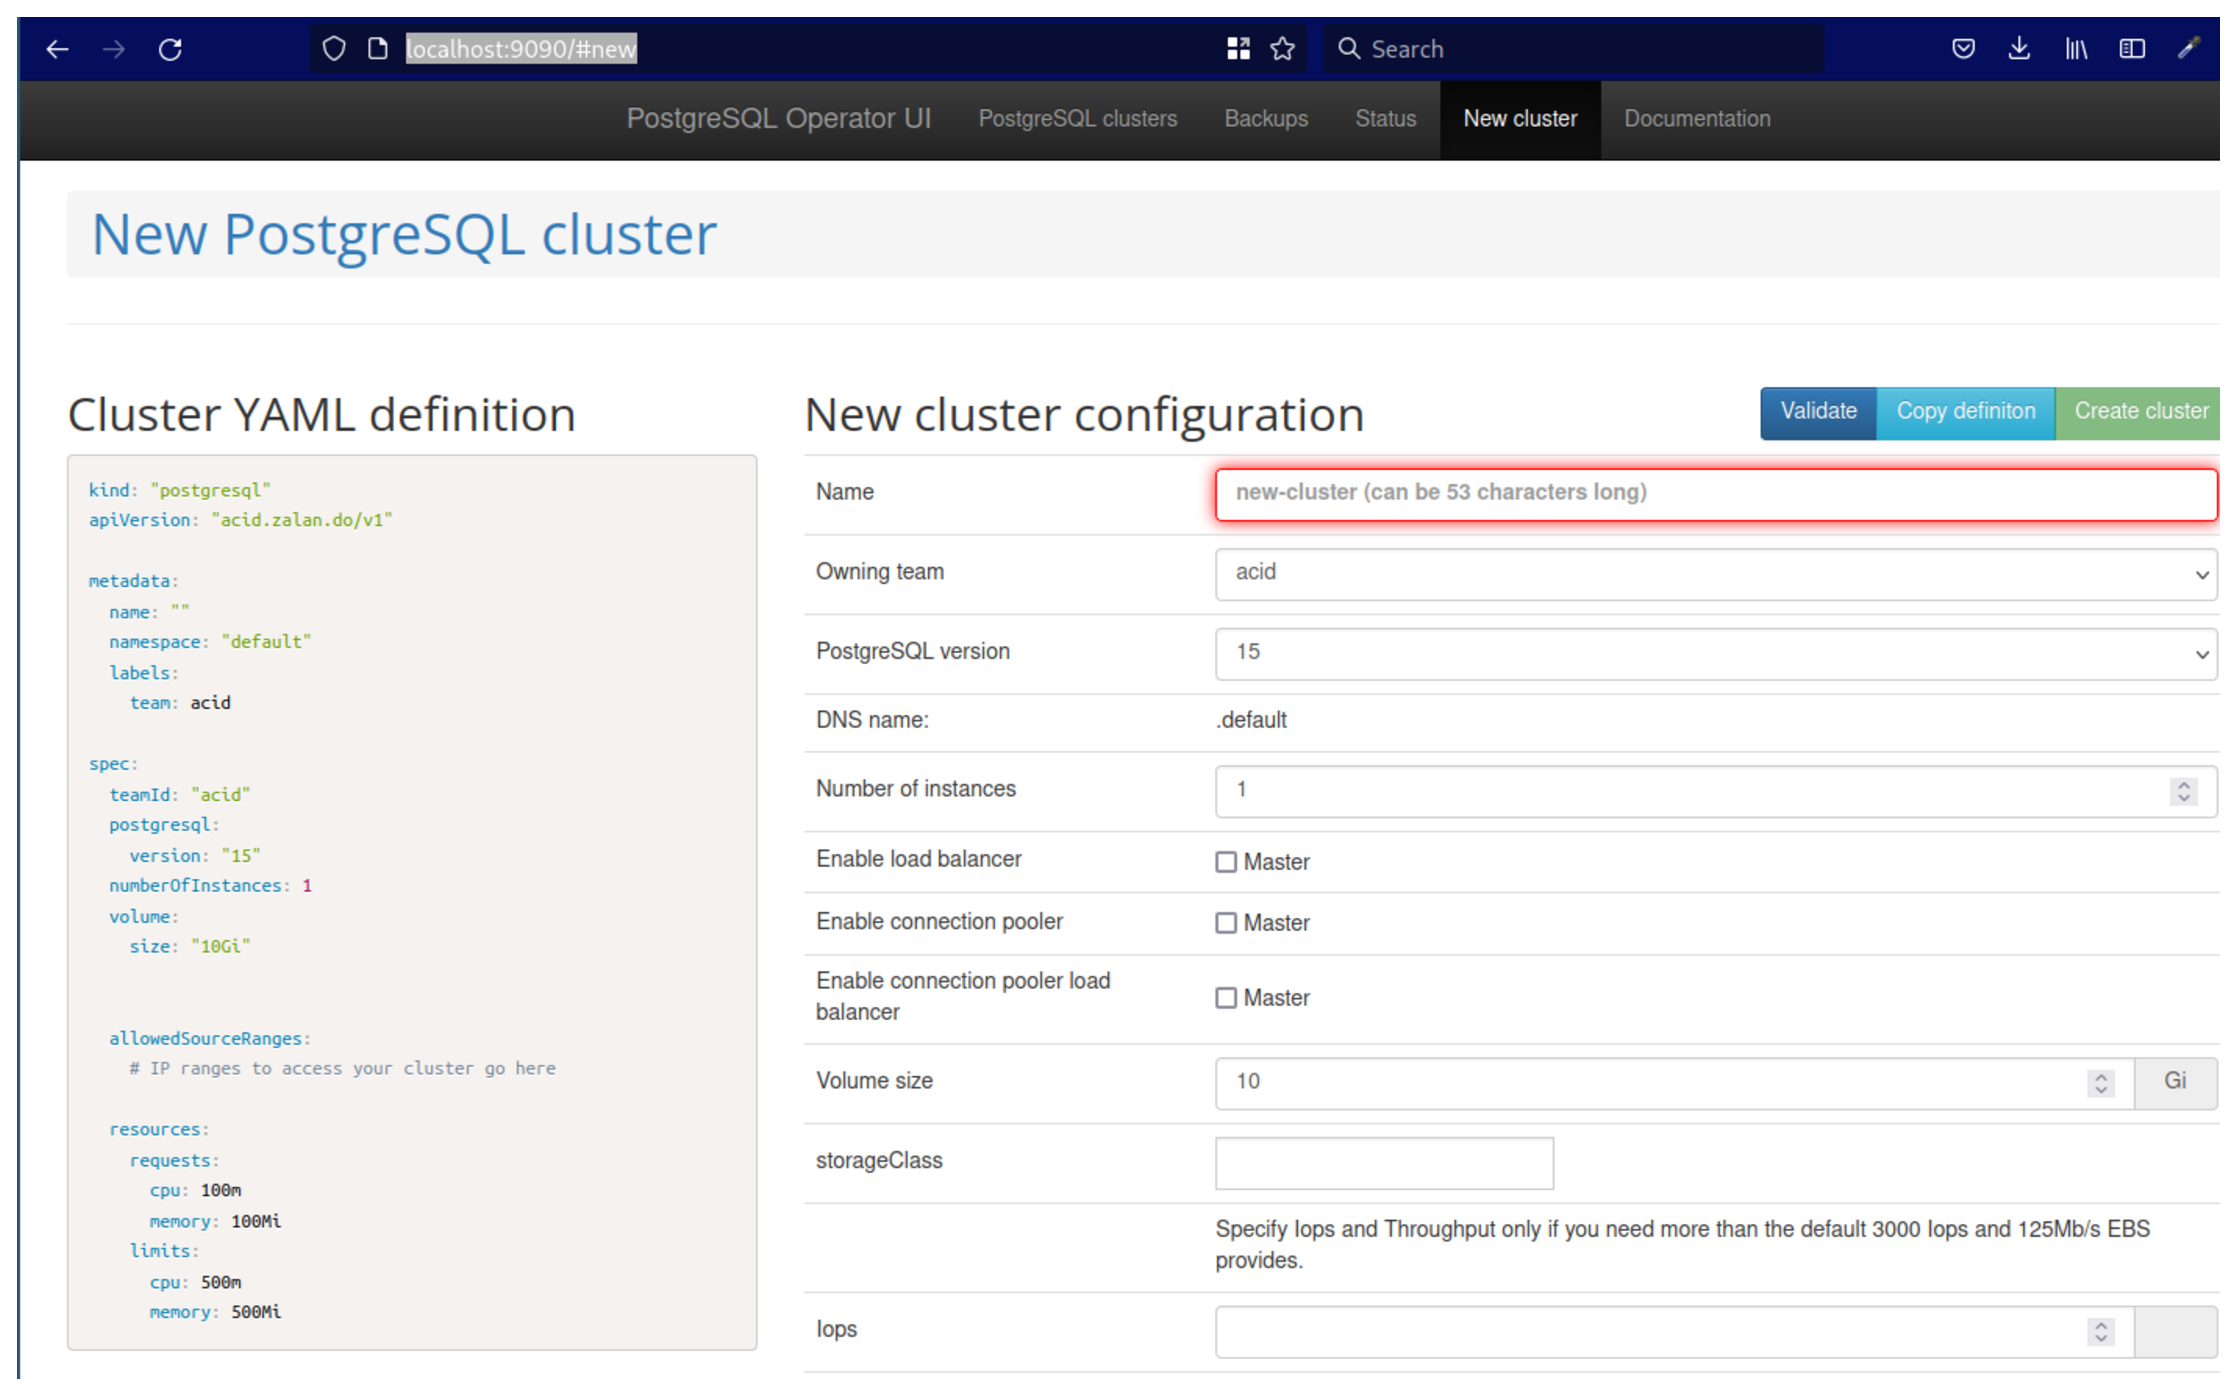
\includegraphics[angle=0, width=0.9\textwidth, height=0.9\textheight]{images/postgres-operator-ui.eps}
\end{center}
\end{figure}

\end{frame}

%%%%%%%%%%%%%%%%%%%%%%%%%%%%%%%%%%%%%%%%%%%%%%%%%%%%%%%%%%%%%%%%%%%%%%%%%%%%%%%%

\begin{frame}[fragile]{Fonctionnalités proposées par l'interface web de l'opérateur PostgreSQL}

L'UI permet de:
\begin{itemize}
   \item choisir la version PostgreSQL (jusquà la version 15 actuellement)
   \item le nombre d'instances
   \item activation du load-balancer
   \item activation du pool de connexions à la base
   \item activation du load-balancer pour le pool de connexions à la base
   \item taille du volume persistent alloué à la base de données
   \item choix du storageClass
   \item performances IO
   \item choix des ressources (demandées et limites) CPU et RAM allouées
\end{itemize}

\end{frame}

%%%%%%%%%%%%%%%%%%%%%%%%%%%%%%%%%%%%%%%%%%%%%%%%%%%%%%%%%%%%%%%%%%%%%%%%%%%%%%%%

\begin{frame}[fragile]{Utilisation de la commande en ligne pour la création d'un cluster PostgreSQL}

   \begin{itemize}
      \item Les fonctionnalités proposées par l'UI sont également disponibles par la commande en ligne.
      \item Le manifeste \textit{manifests/complete-postgresql-manifest.yaml} permet de préciser l'ensemble des paramètres proposés par l'UI.
      \item Pour appliquer ce manifeste \textit{manifests/complete-postgresql-manifest.yaml}, la commande suivante est lancée sur le n\oe{}ud:
\begin{tiny}
\begin{Verbatim}[commandchars=\&\{\}]
kubectl create -f manifests/complete-postgresql-manifest.yaml
\end{Verbatim}
\end{tiny}
   \end{itemize}

\end{frame}

%%%%%%%%%%%%%%%%%%%%%%%%%%%%%%%%%%%%%%%%%%%%%%%%%%%%%%%%%%%%%%%%%%%%%%%%%%%%%%%%

\begin{frame}[fragile]{Vérification de l'état du cluster PostgreSQL}

\begin{tiny}
\begin{Verbatim}[commandchars=\&\{\}]
$ kubectl get pods -l application=spilo -L spilo-role
NAME                  READY   STATUS    RESTARTS   AGE   SPILO-ROLE
acid-test-cluster-0   1/1     Running   0          12m   
acid-test-cluster-1   1/1     Running   0          10m   
$ kubectl get postgresql
NAME                TEAM   VERSION   PODS   VOLUME   CPU-REQUEST   MEMORY-REQUEST   AGE   STATUS
acid-test-cluster   acid   15        2      1Gi      10m           100Mi            68d   Running
$ kubectl get pods -l application=spilo -L spilo-role
NAME                  READY   STATUS    RESTARTS   AGE   SPILO-ROLE
acid-test-cluster-0   1/1     Running   0          13m   
acid-test-cluster-1   1/1     Running   0          10m   
$ kubectl get svc -l application=spilo -L spilo-role
NAME                       TYPE        CLUSTER-IP      EXTERNAL-IP   PORT(S)    AGE   SPILO-ROLE
acid-test-cluster          ClusterIP   10.103.247.68   <none>        5432/TCP   68d   master
acid-test-cluster-config   ClusterIP   None            <none>        <none>     68d   
acid-test-cluster-repl     ClusterIP   10.100.95.205   <none>        5432/TCP   68d   replica
\end{Verbatim}
\end{tiny}

\end{frame}

%%%%%%%%%%%%%%%%%%%%%%%%%%%%%%%%%%%%%%%%%%%%%%%%%%%%%%%%%%%%%%%%%%%%%%%%%%%%%%%%

\begin{frame}[fragile]{Déploiement de \textbf{krew}}

\begin{tiny}
\begin{Verbatim}[commandchars=\&\#\#]
(
  set -x; cd "$(mktemp -d)" &&
  OS="$(uname | tr '[:upper:]' '[:lower:]')" &&
  ARCH="$(uname -m | sed -e 's/x86_64/amd64/' -e 's/\(arm\)\(64\)\?.*/\1\2/' -e 's/aarch64$/arm64/')" &&
  KREW="krew-${OS}_${ARCH}" &&
  curl -fsSLO "https://github.com/kubernetes-sigs/krew/releases/latest/download/${KREW}.tar.gz" &&
  tar zxvf "${KREW}.tar.gz" &&
  ./"${KREW}" install krew
)
\end{Verbatim}
\end{tiny}

\end{frame}

%%%%%%%%%%%%%%%%%%%%%%%%%%%%%%%%%%%%%%%%%%%%%%%%%%%%%%%%%%%%%%%%%%%%%%%%%%%%%%%%

\begin{frame}[fragile]{Déploiement de \textbf{krew}}

   Ajout du répertoire des binaires du paquet krew dans \textbf{.bashrc} ou \textbf{.zshrc}:

\begin{tiny}
\begin{Verbatim}[commandchars=\&\#\#]
export PATH="${KREW_ROOT:-$HOME/.krew}/bin:$PATH"
\end{Verbatim}
\end{tiny}

Redémarrer le shell.\\
Pour vérifier le déploiement correct de krew, lancer la commande suivante:

\begin{tiny}
\begin{Verbatim}[commandchars=\&\#\#]
kubectl krew
\end{Verbatim}
\end{tiny}

\end{frame}

%%%%%%%%%%%%%%%%%%%%%%%%%%%%%%%%%%%%%%%%%%%%%%%%%%%%%%%%%%%%%%%%%%%%%%%%%%%%%%%%

\begin{frame}[fragile]{Déploiement de l'opérateur Minio}

   Le déploiement de Minio s'appuie sur l'opérateur Minio.\\
   Son déploiement est décrit dans le lien suivant \url{https://operator.min.io/#architecture}.\\

\begin{tiny}
\begin{Verbatim}[commandchars=\&\#\#]
kubectl krew update
kubectl krew install minio
\end{Verbatim}
\end{tiny}


\end{frame}

%%%%%%%%%%%%%%%%%%%%%%%%%%%%%%%%%%%%%%%%%%%%%%%%%%%%%%%%%%%%%%%%%%%%%%%%%%%%%%%%

\begin{frame}[fragile]{Vérification de l'état de l'opérateur Minio}

\begin{tiny}
\begin{Verbatim}[commandchars=\\\{\}]
$ kubectl get pods -n minio-operator
NAME                              READY   STATUS    RESTARTS           AGE
console-56f9795d5c-59fsx          1/1     \textbf{Running}   1 (33d ago)        82d
minio-operator-7cd6784f59-5c52w   1/1     \textbf{Running}   5 (23h ago)        17d
minio-operator-7cd6784f59-m7h8x   1/1     \textbf{Running}   2320 (3d16h ago)   82d
\end{Verbatim}
\end{tiny}

\end{frame}

%%%%%%%%%%%%%%%%%%%%%%%%%%%%%%%%%%%%%%%%%%%%%%%%%%%%%%%%%%%%%%%%%%%%%%%%%%%%%%%%

\begin{frame}[fragile]{Accès à la console Minio}

   La commande suivante ouvre un accès de type proxy à la console Minio:
\begin{tiny}
\begin{Verbatim}[commandchars=\&\#\#]
$ kubectl minio proxy -n minio-operator
Starting port forward of the Console UI.

To connect open a browser and go to http://localhost:9090

Current JWT to login: *****

Forwarding from 0.0.0.0:9090 -> 9090
Handling connection for 9090

\end{Verbatim}
\end{tiny}

Depuis le terminal de l'utilisateur, lancer la commande suivante:

\begin{tiny}
\begin{Verbatim}[commandchars=\&\#\#]
$ ssh -L 9090:localhost:9090 dgfip-k8s
\end{Verbatim}
\end{tiny}

\end{frame}

%%%%%%%%%%%%%%%%%%%%%%%%%%%%%%%%%%%%%%%%%%%%%%%%%%%%%%%%%%%%%%%%%%%%%%%%%%%%%%%%

\begin{frame}[fragile]{Accès à la console Minio}

   Dans le champ \textit{Enter JWT}, renseigner la valeur du token JWT renvoyé par la commande précédente:
\begin{figure}
\begin{center}
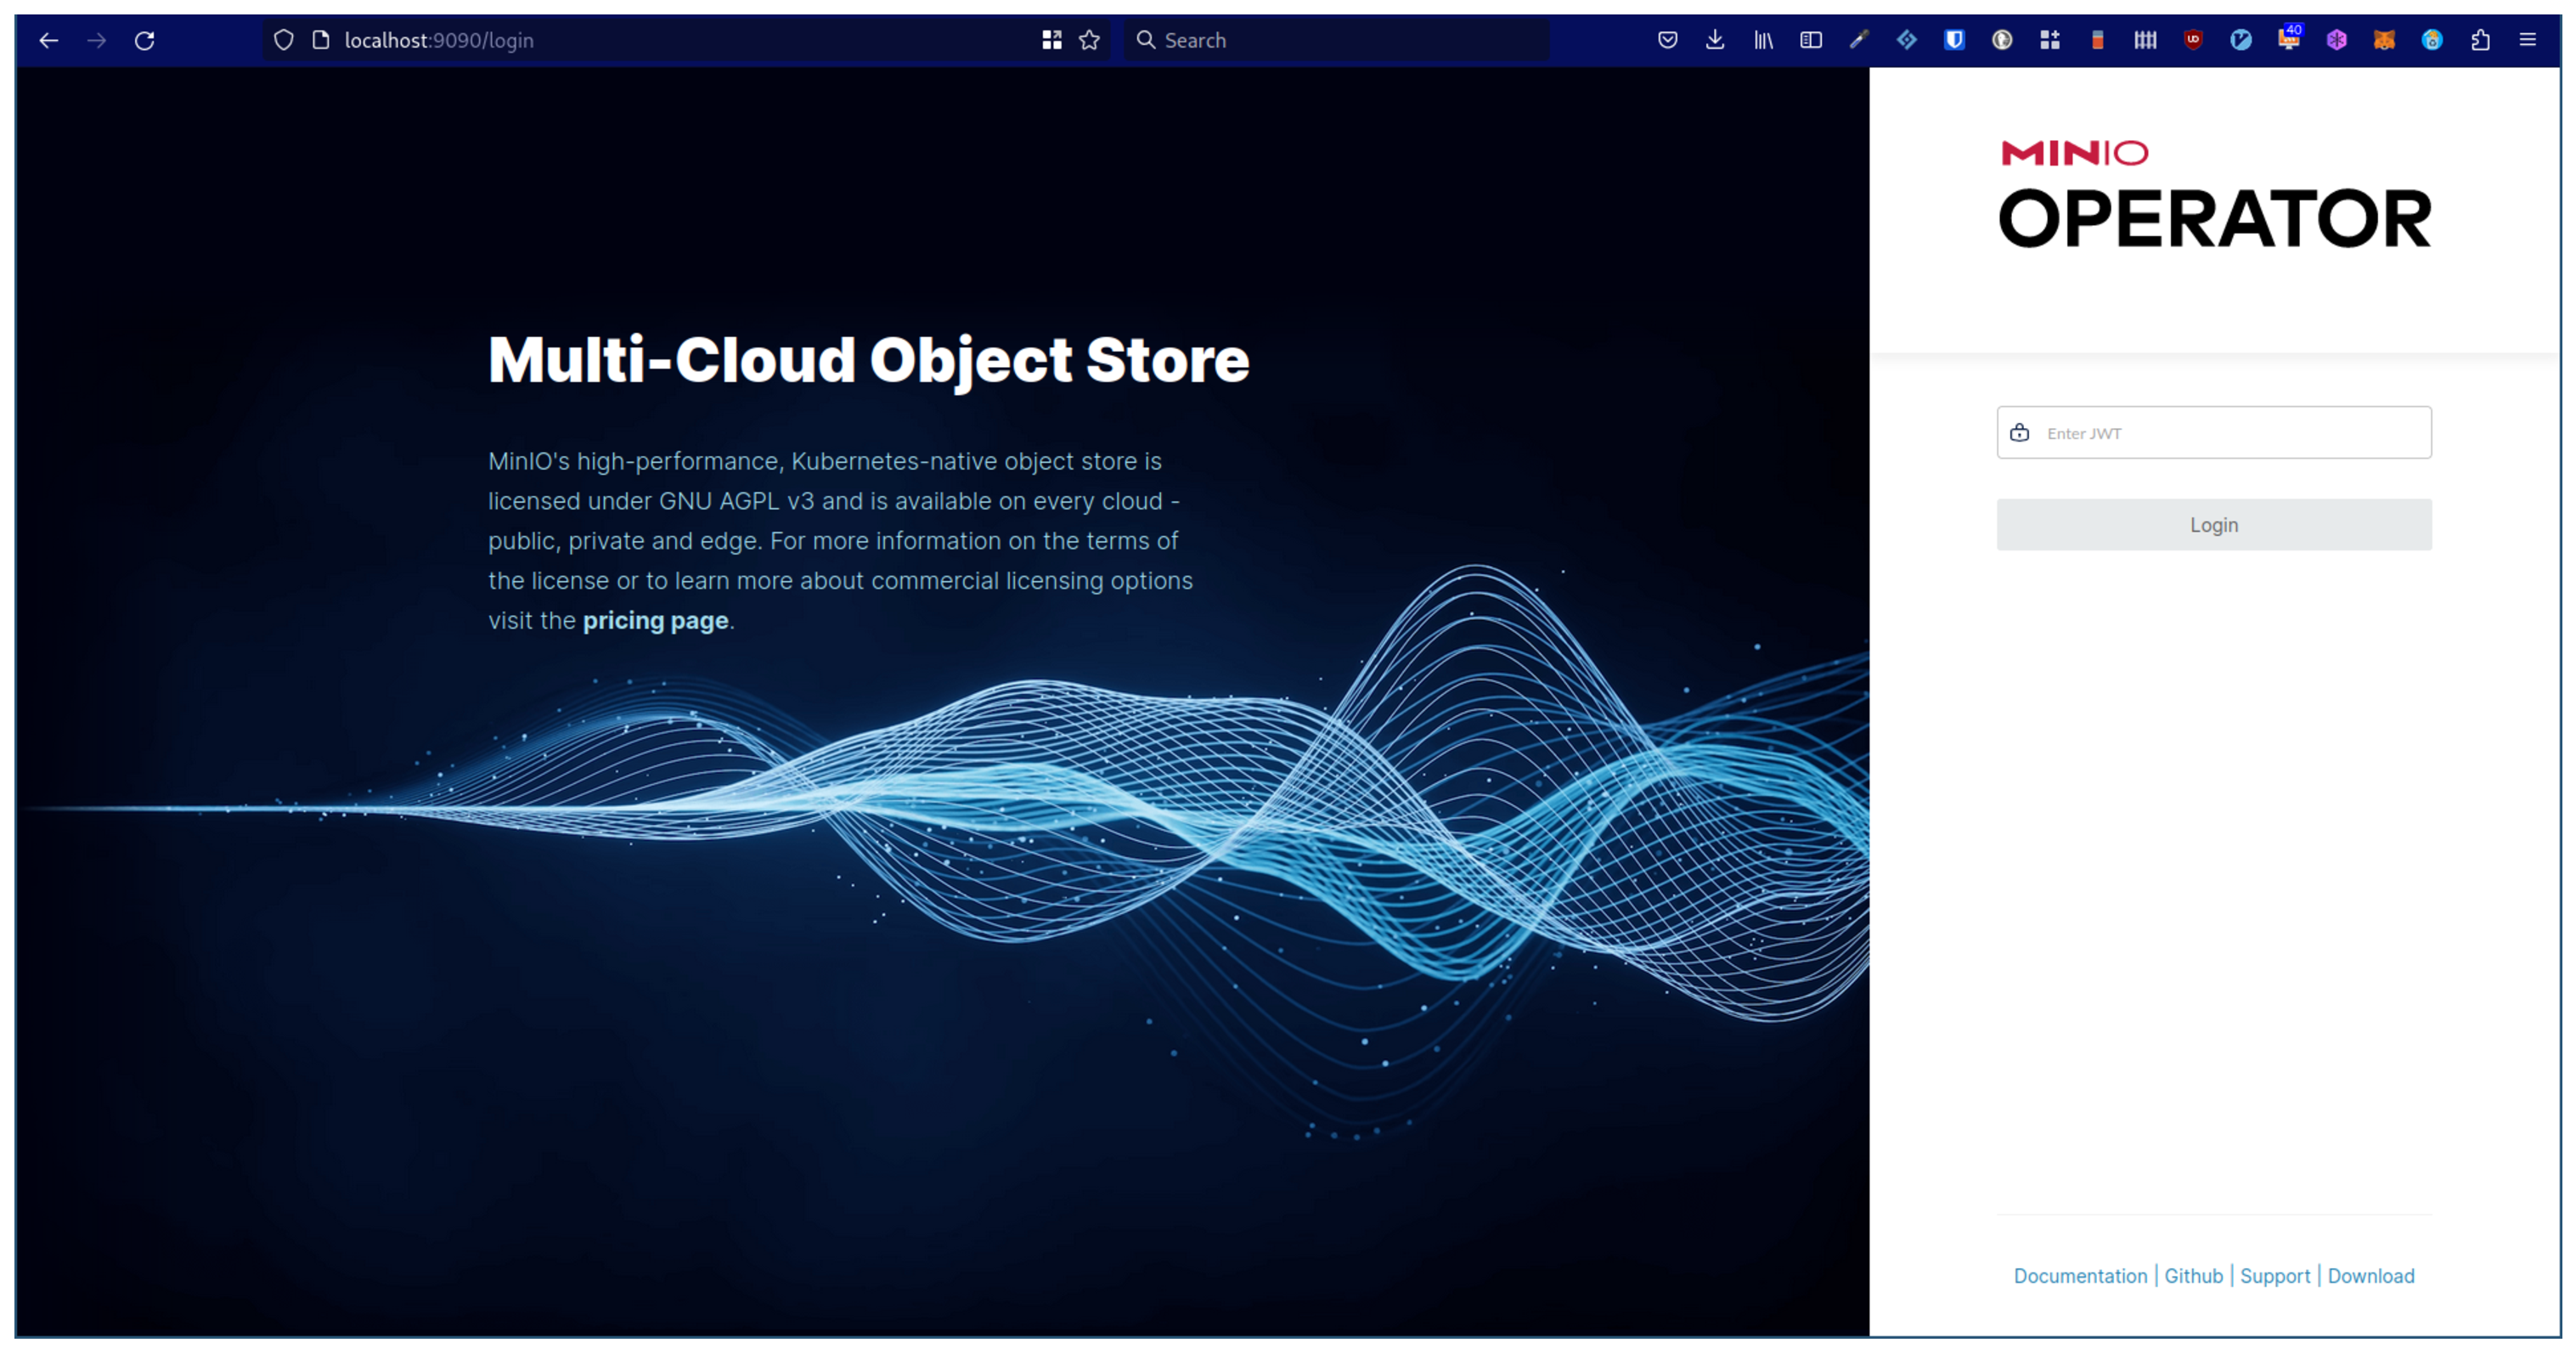
\includegraphics[angle=0, width=0.9\textwidth, height=0.7\textheight]{images/login_console_minio.eps}
\end{center}
\end{figure}

\end{frame}

%%%%%%%%%%%%%%%%%%%%%%%%%%%%%%%%%%%%%%%%%%%%%%%%%%%%%%%%%%%%%%%%%%%%%%%%%%%%%%%%

\begin{frame}[fragile]{Dashboard Minio}

   Le tableau de bord de Minio ressemble à ceci:
\begin{figure}
\begin{center}
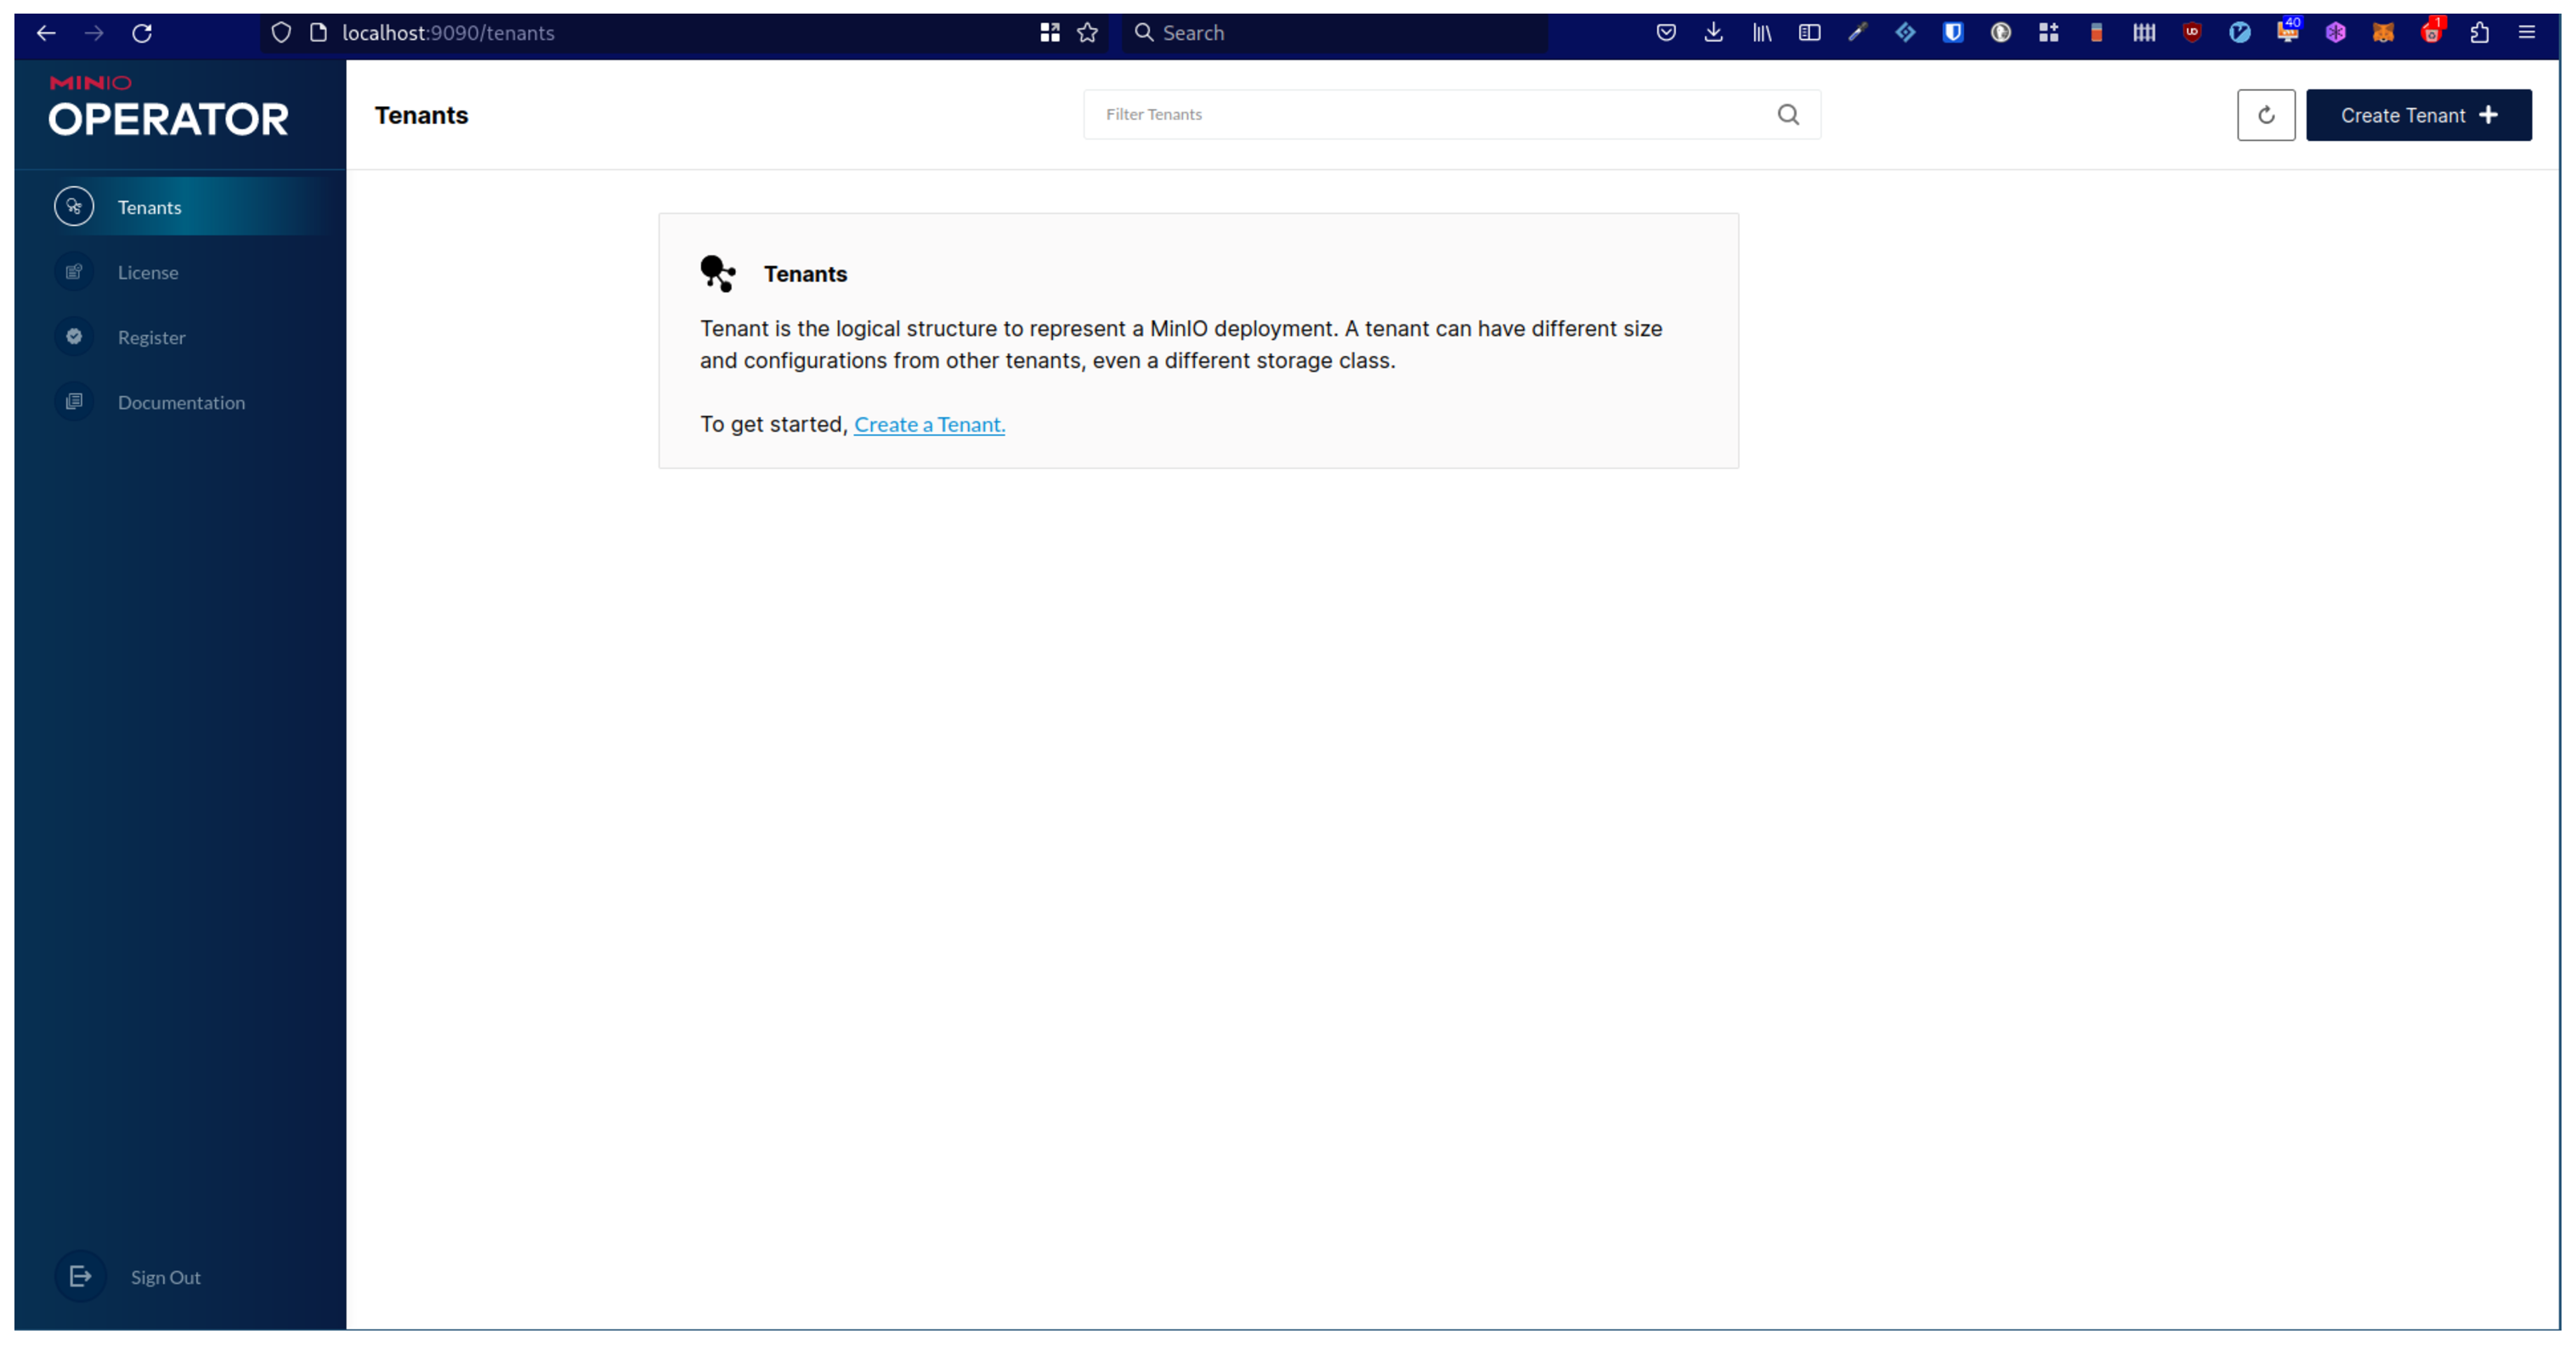
\includegraphics[angle=0, width=0.9\textwidth, height=0.8\textheight]{images/console_minio.eps}
\end{center}
\end{figure}

\end{frame}

%%%%%%%%%%%%%%%%%%%%%%%%%%%%%%%%%%%%%%%%%%%%%%%%%%%%%%%%%%%%%%%%%%%%%%%%%%%%%%%%

\begin{frame}[fragile]{Création d'un tenant - Setup - Minio}

\begin{figure}
\begin{center}
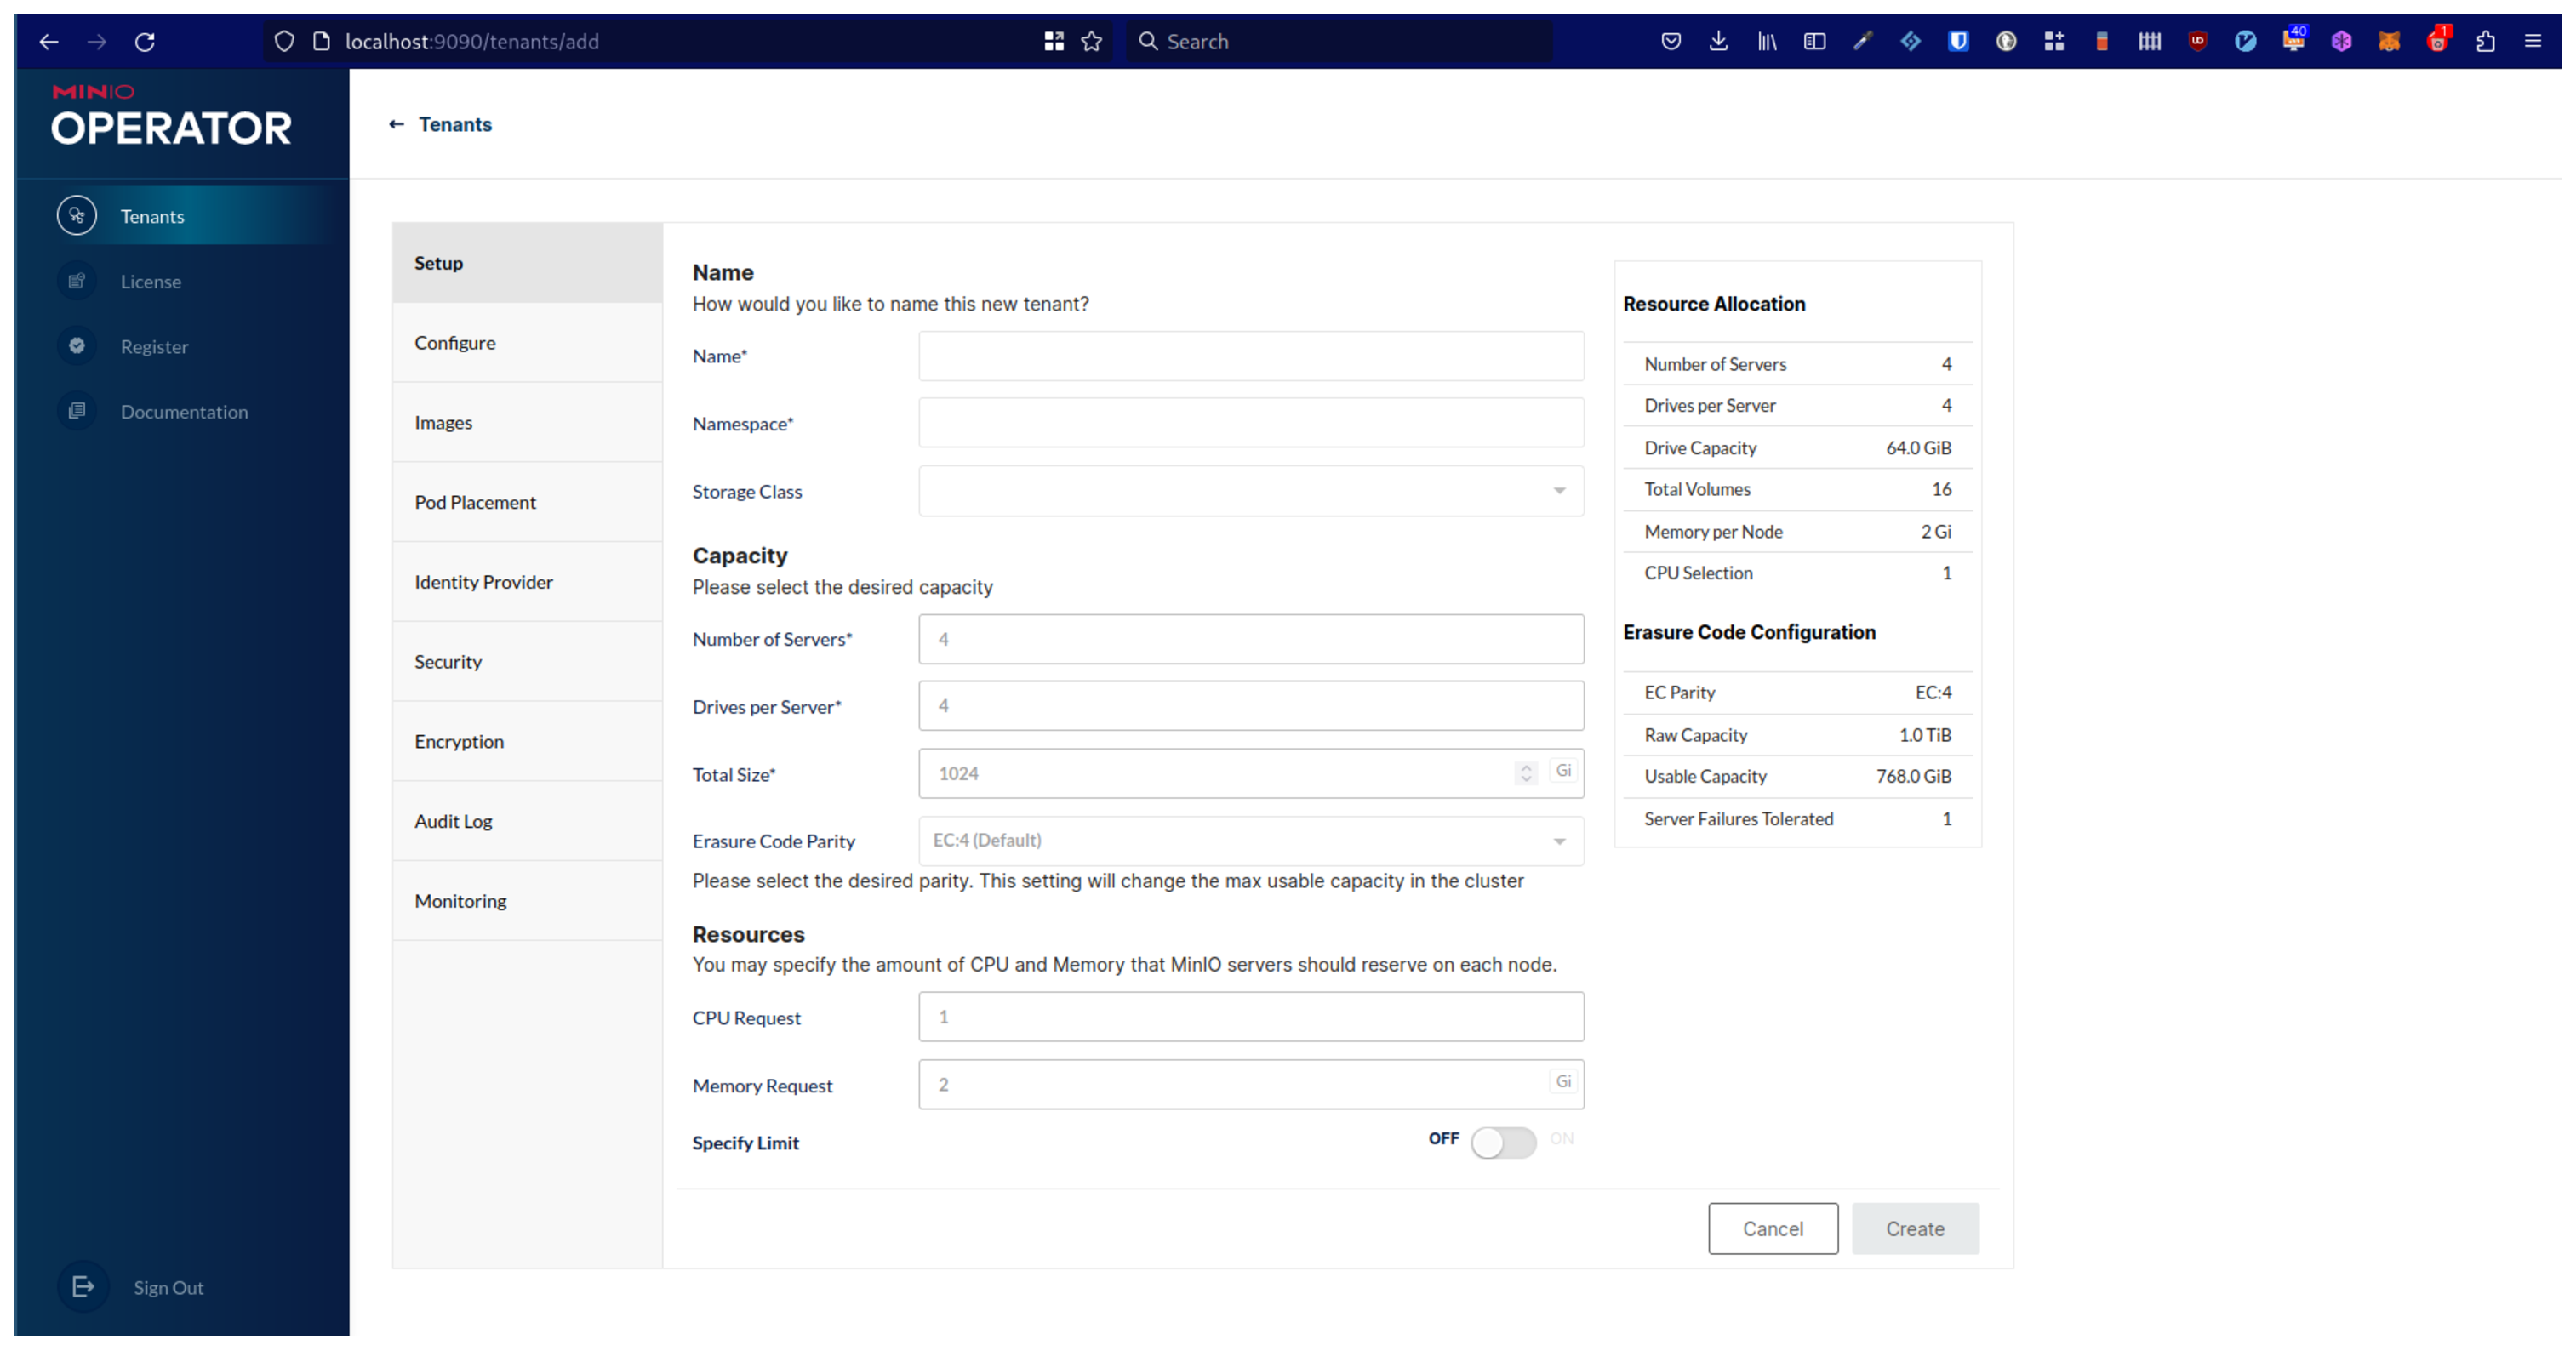
\includegraphics[angle=0, width=0.9\textwidth, height=0.8\textheight]{images/setup_minio.eps}
\end{center}
\end{figure}

\end{frame}

%%%%%%%%%%%%%%%%%%%%%%%%%%%%%%%%%%%%%%%%%%%%%%%%%%%%%%%%%%%%%%%%%%%%%%%%%%%%%%%%

\begin{frame}[fragile]{Création d'un tenant - Configure - Minio}

\begin{figure}
\begin{center}
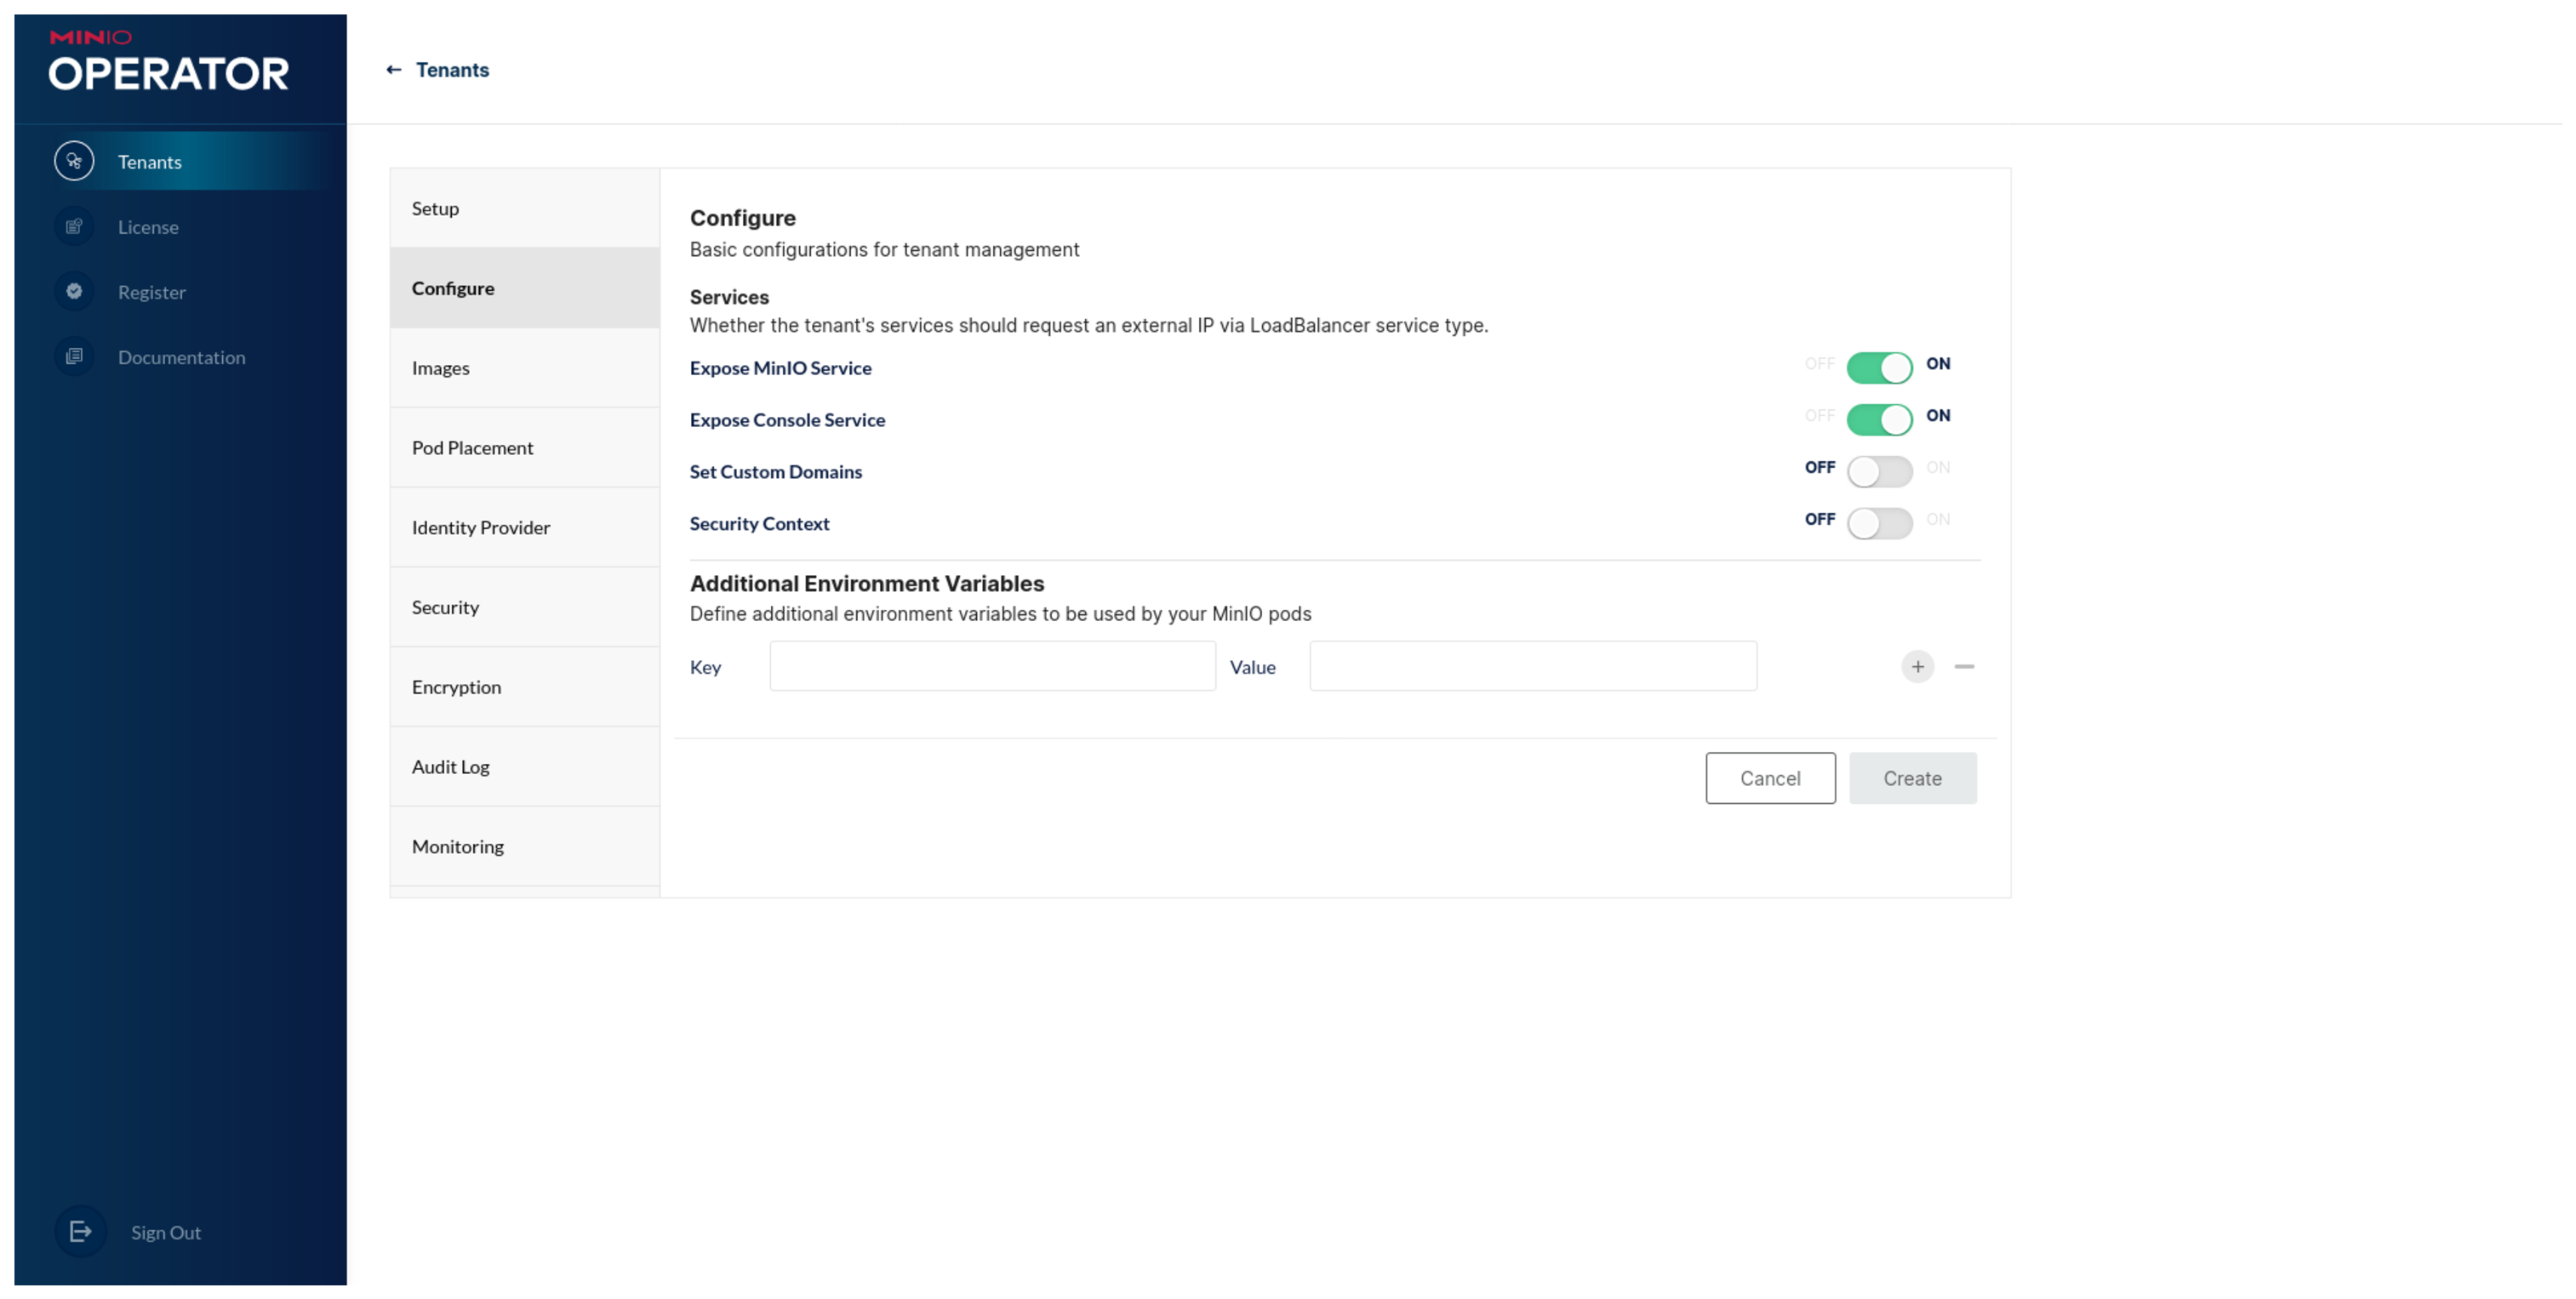
\includegraphics[angle=0, width=0.9\textwidth, height=0.8\textheight]{images/configure_minio.eps}
\end{center}
\end{figure}

\end{frame}

%%%%%%%%%%%%%%%%%%%%%%%%%%%%%%%%%%%%%%%%%%%%%%%%%%%%%%%%%%%%%%%%%%%%%%%%%%%%%%%%

\begin{frame}[fragile]{Marquage des n\oe{}uds Minio}

   Depuis le control plane, lancer les commandes suivantes pour marquer les n\oe{}uds:
\begin{tiny}
\begin{Verbatim}[commandchars=\\\{\}]
$ kubectl label nodes dnumminioworker1 role=s3-node
node/dnumminioworker1 labeled
$ kubectl label nodes dnumminioworker2 role=s3-node
node/dnumminioworker2 labeled
$ kubectl label nodes dnumminioworker3 role=s3-node
node/dnumminioworker3 labeled
$ kubectl label nodes dnumminioworker4 role=s3-node
node/dnumminioworker4 labeled
\end{Verbatim}
\end{tiny}

   Affichage du label des n\oe{}uds:
\begin{tiny}
\begin{Verbatim}[commandchars=\\\{\}]
$ kubectl get nodes --show-labels
NAME               STATUS   ROLES           AGE    VERSION   LABELS
\ldots
dnumminioworker1   Ready    <none>          6h2m   v1.27.2   \ldots,\textbf{role=s3-node}
dnumminioworker2   Ready    <none>          142m   v1.27.2   \ldots,\textbf{role=s3-node}
dnumminioworker3   Ready    <none>          109m   v1.27.2   \ldots,\textbf{role=s3-node}
dnumminioworker4   Ready    <none>          83m    v1.27.2   \ldots,\textbf{role=s3-node}
\ldots

\end{Verbatim}
\end{tiny}

\end{frame}

%%%%%%%%%%%%%%%%%%%%%%%%%%%%%%%%%%%%%%%%%%%%%%%%%%%%%%%%%%%%%%%%%%%%%%%%%%%%%%%%

\begin{frame}[fragile]{Création d'un tenant - Pod placement - Minio}

\begin{figure}
\begin{center}
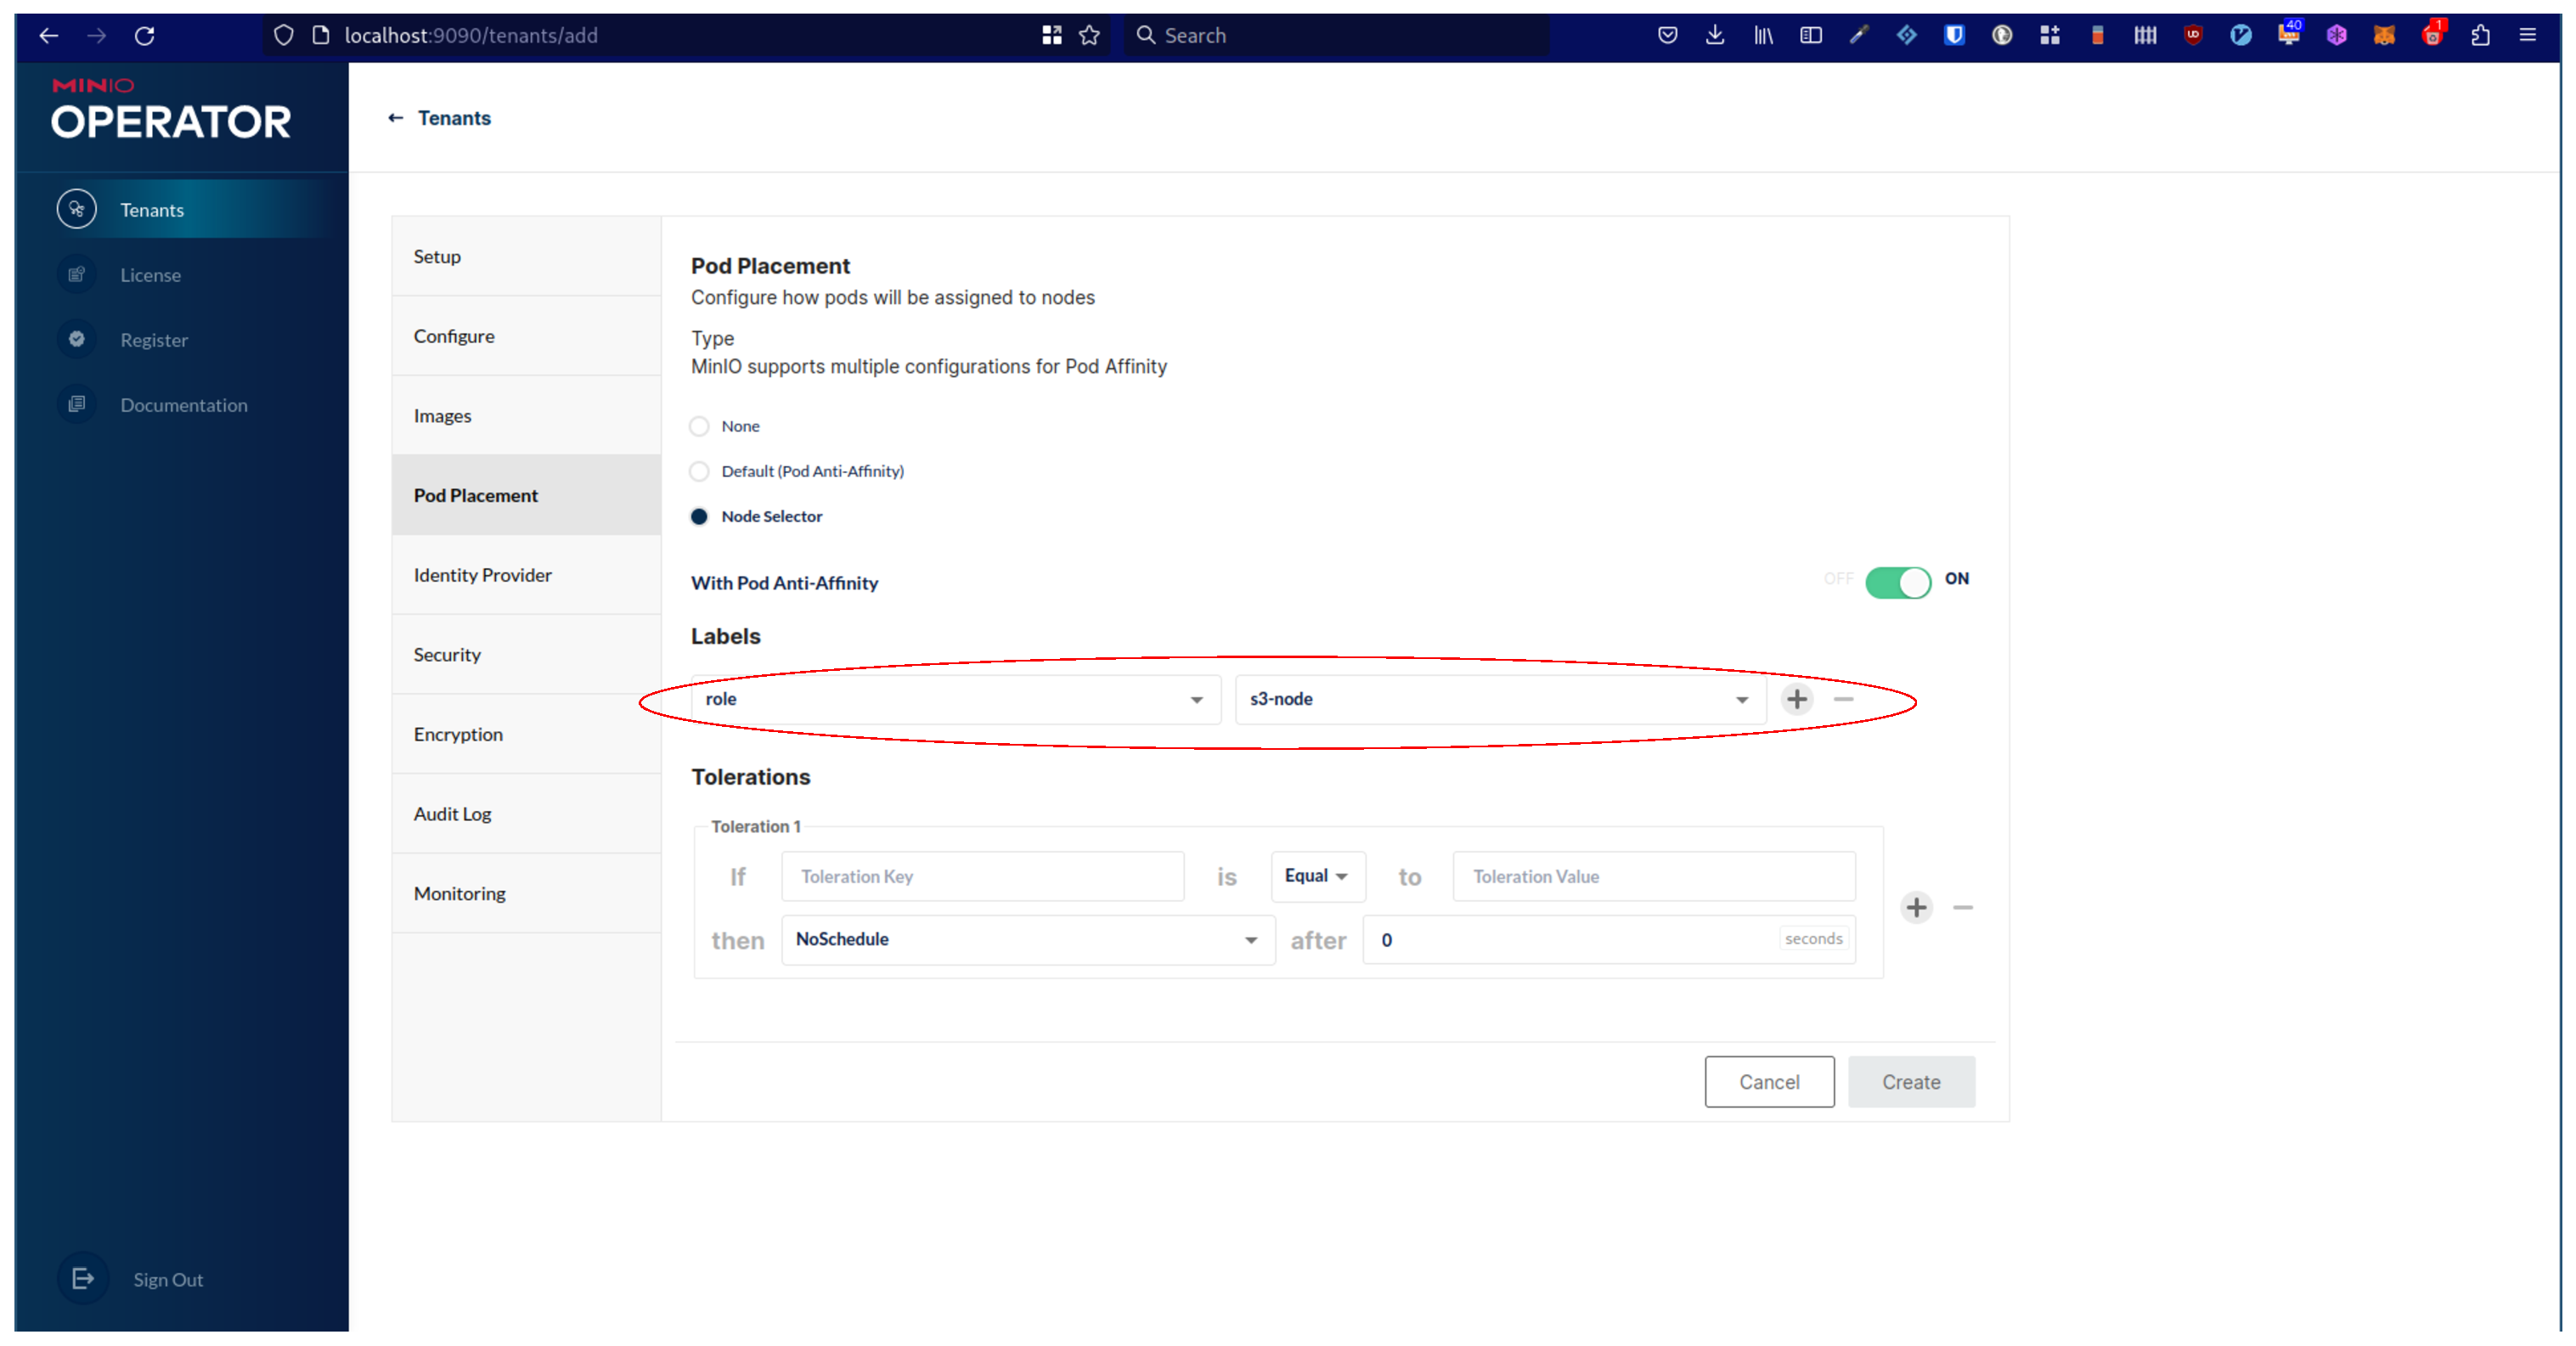
\includegraphics[angle=0, width=0.9\textwidth, height=0.9\textheight]{images/pod_placement.eps}
\end{center}
\end{figure}

\end{frame}

%%%%%%%%%%%%%%%%%%%%%%%%%%%%%%%%%%%%%%%%%%%%%%%%%%%%%%%%%%%%%%%%%%%%%%%%%%%%%%%%

\begin{frame}[fragile]{Création d'un tenant - Choix d'un fournisseur d'identité - Minio}

\begin{figure}
\begin{center}
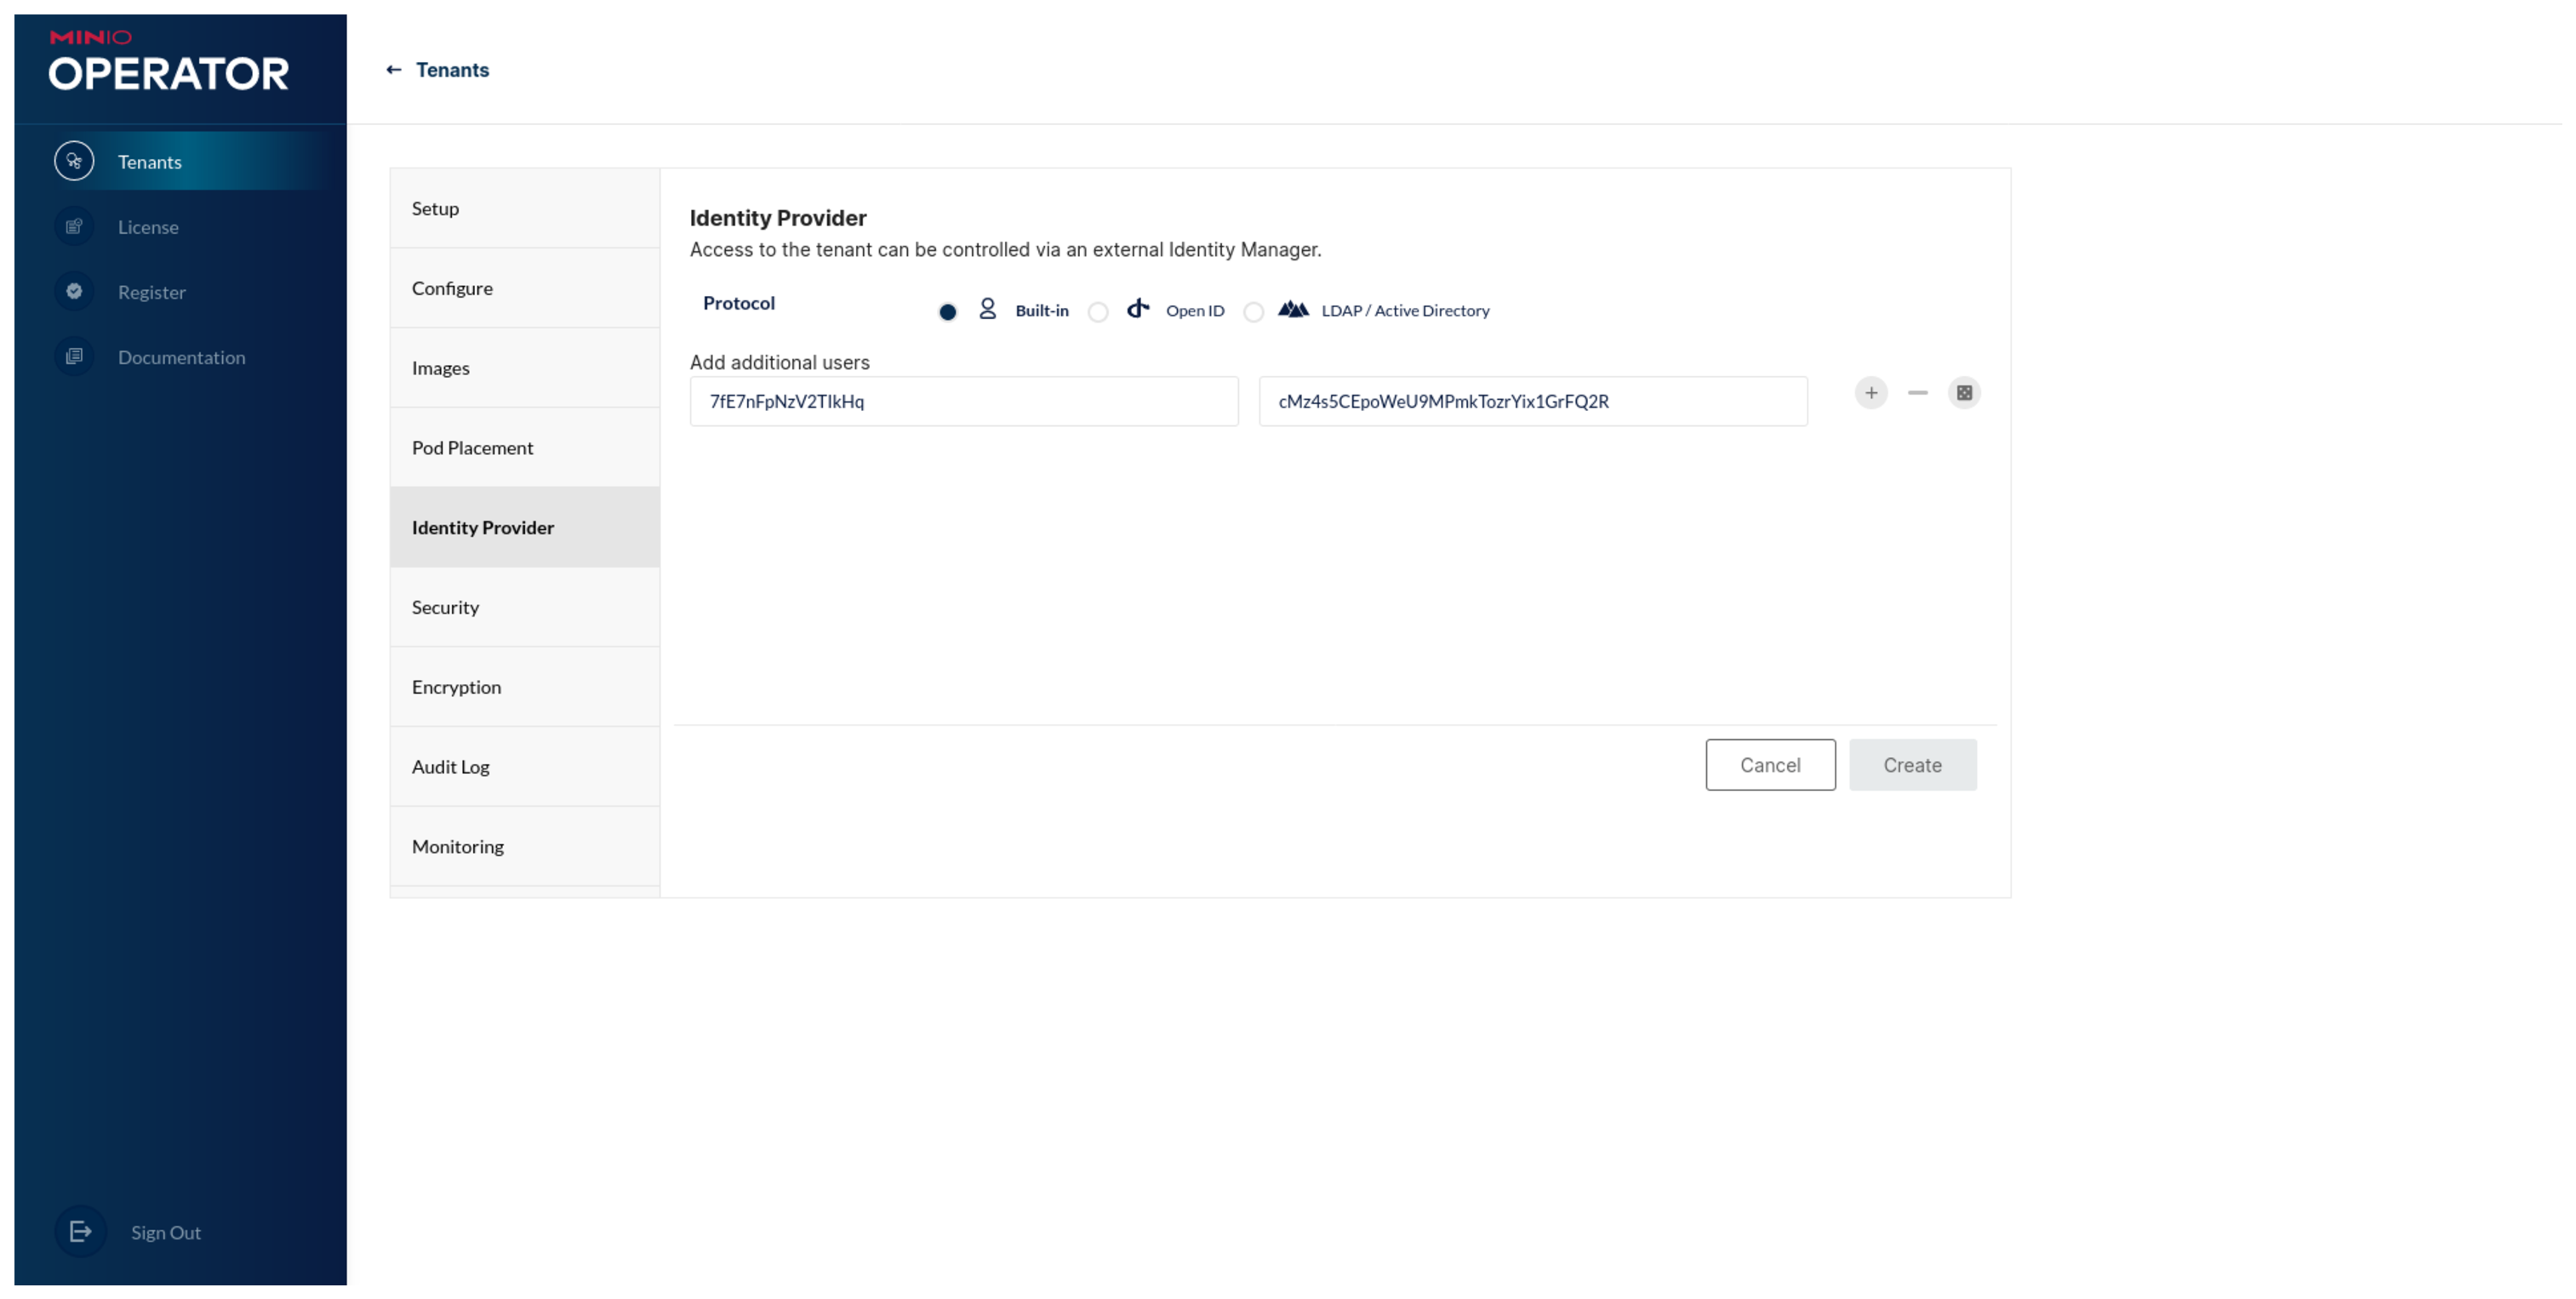
\includegraphics[angle=0, width=0.9\textwidth, height=0.9\textheight]{images/identity_provider_minio.eps}
\end{center}
\end{figure}

\end{frame}

%%%%%%%%%%%%%%%%%%%%%%%%%%%%%%%%%%%%%%%%%%%%%%%%%%%%%%%%%%%%%%%%%%%%%%%%%%%%%%%%

\begin{frame}[fragile]{Création d'un tenant - Sécurité - Minio}

\begin{figure}
\begin{center}
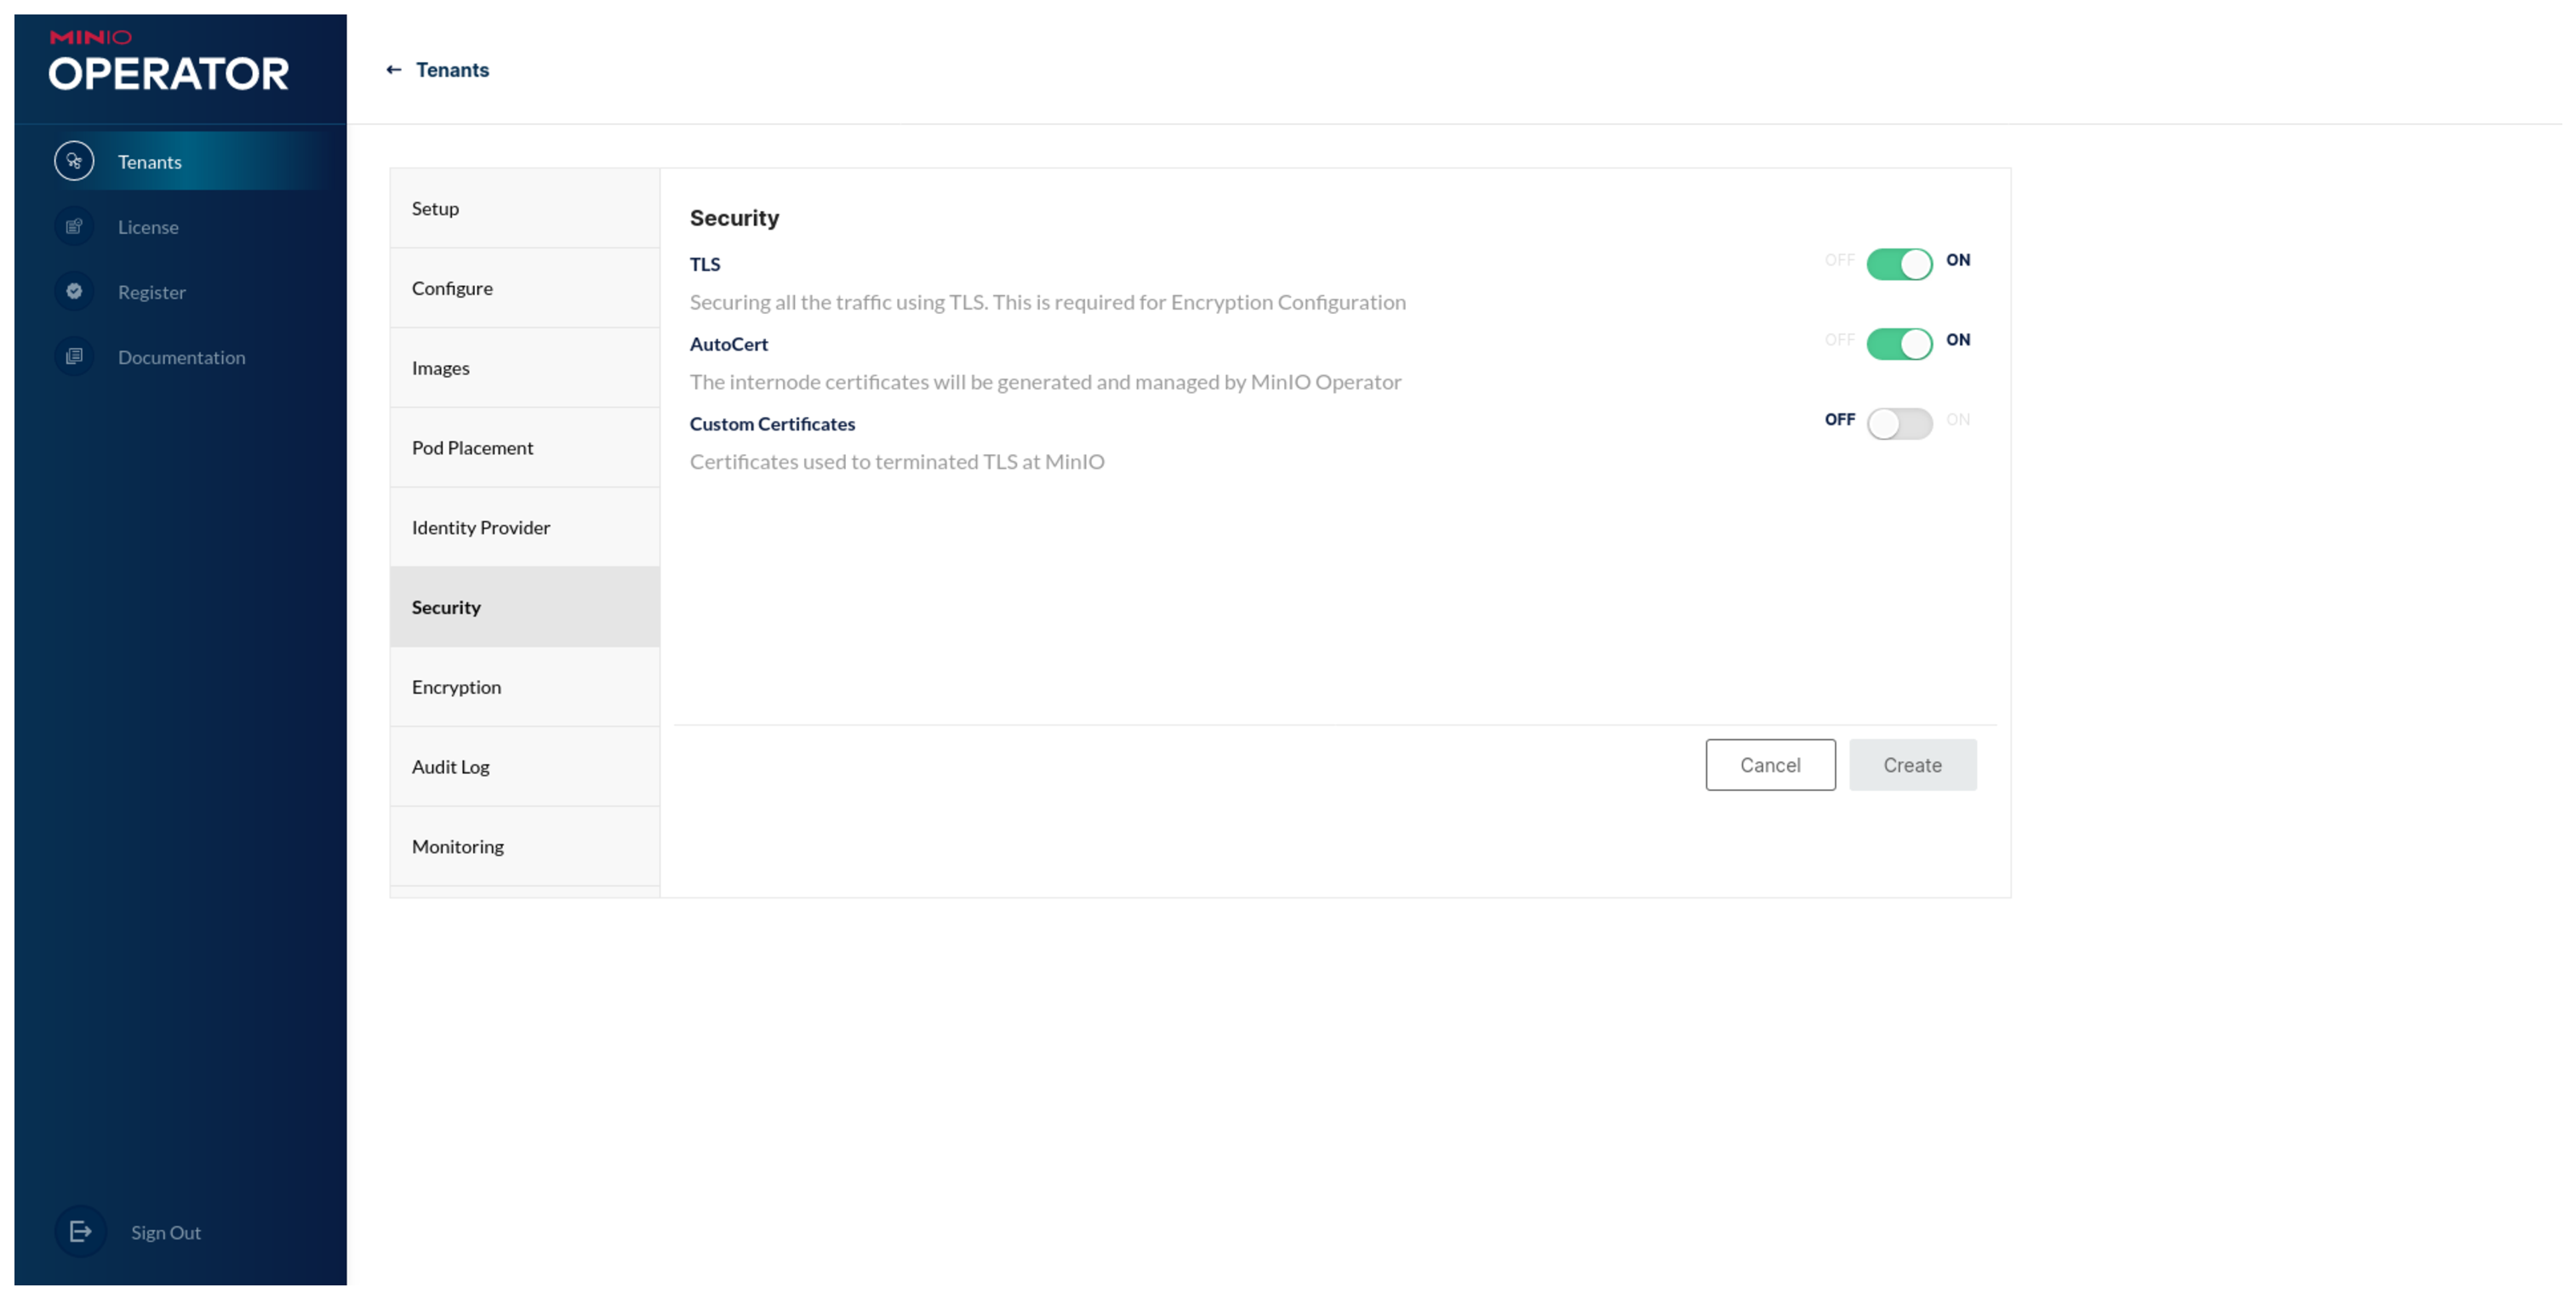
\includegraphics[angle=0, width=0.9\textwidth, height=0.9\textheight]{images/security_minio.eps}
\end{center}
\end{figure}

\end{frame}

%%%%%%%%%%%%%%%%%%%%%%%%%%%%%%%%%%%%%%%%%%%%%%%%%%%%%%%%%%%%%%%%%%%%%%%%%%%%%%%%

\begin{frame}[fragile]{Création d'un tenant - Chiffrement - Minio}

\begin{figure}
\begin{center}
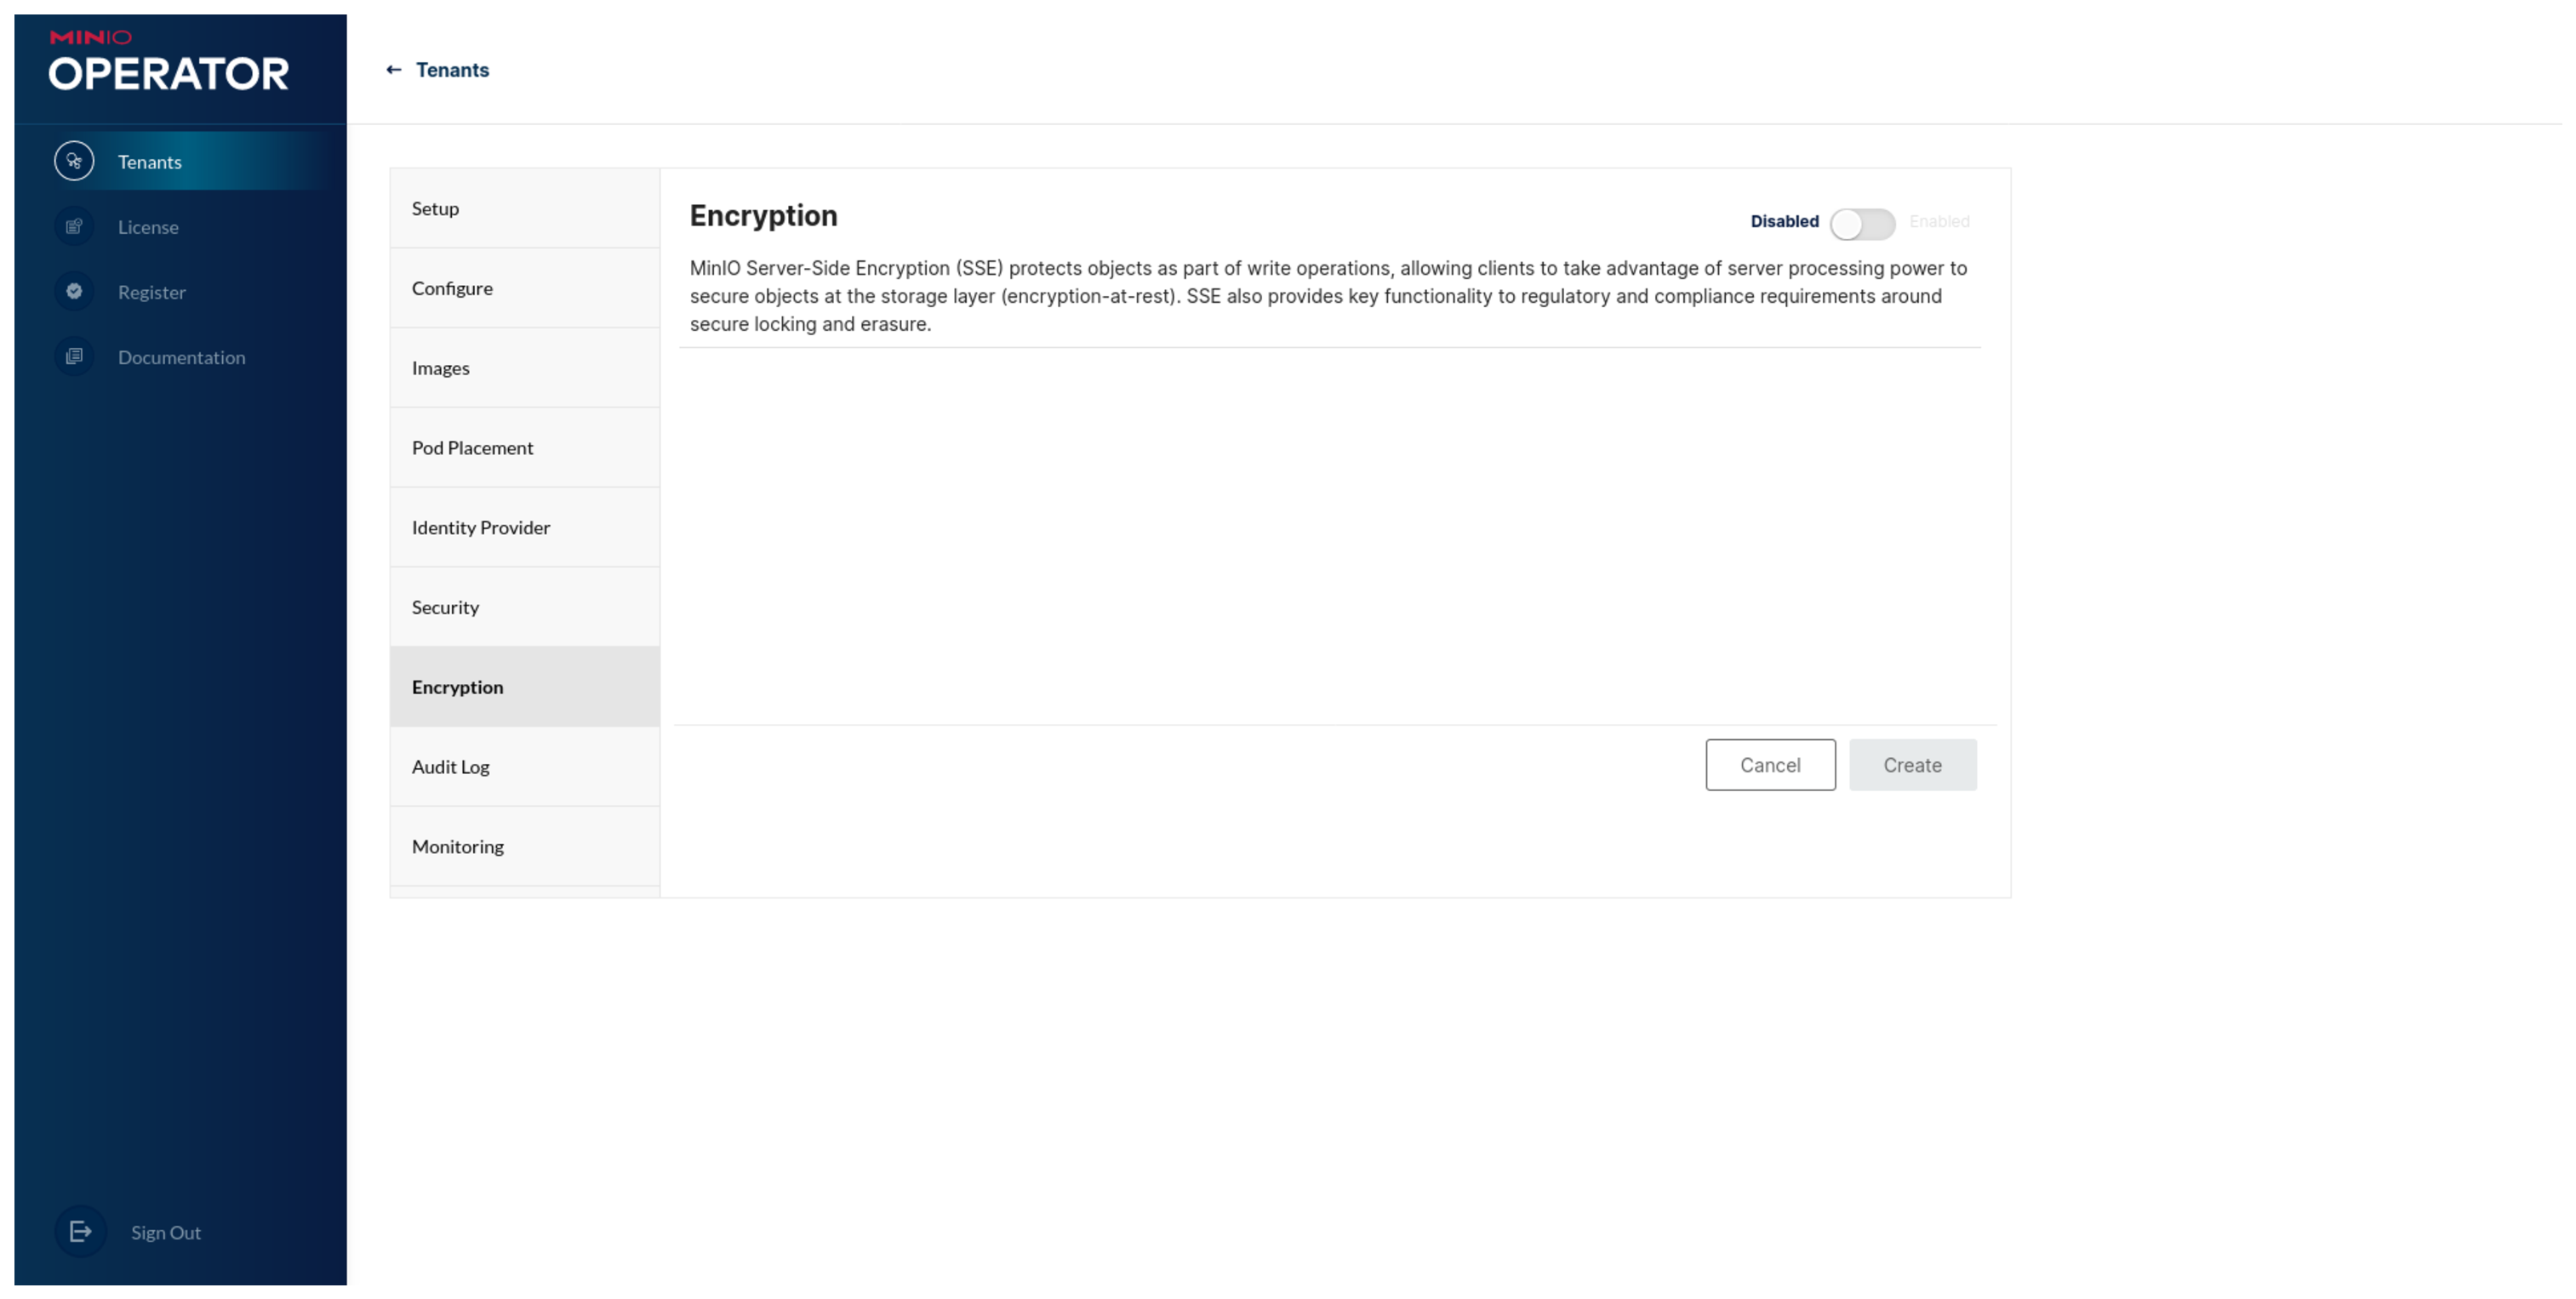
\includegraphics[angle=0, width=0.9\textwidth, height=0.9\textheight]{images/encryption_minio.eps}
\end{center}
\end{figure}

\end{frame}

%%%%%%%%%%%%%%%%%%%%%%%%%%%%%%%%%%%%%%%%%%%%%%%%%%%%%%%%%%%%%%%%%%%%%%%%%%%%%%%%

\begin{frame}[fragile]{Création d'un tenant - Log d'audit - Minio}

\begin{figure}
\begin{center}
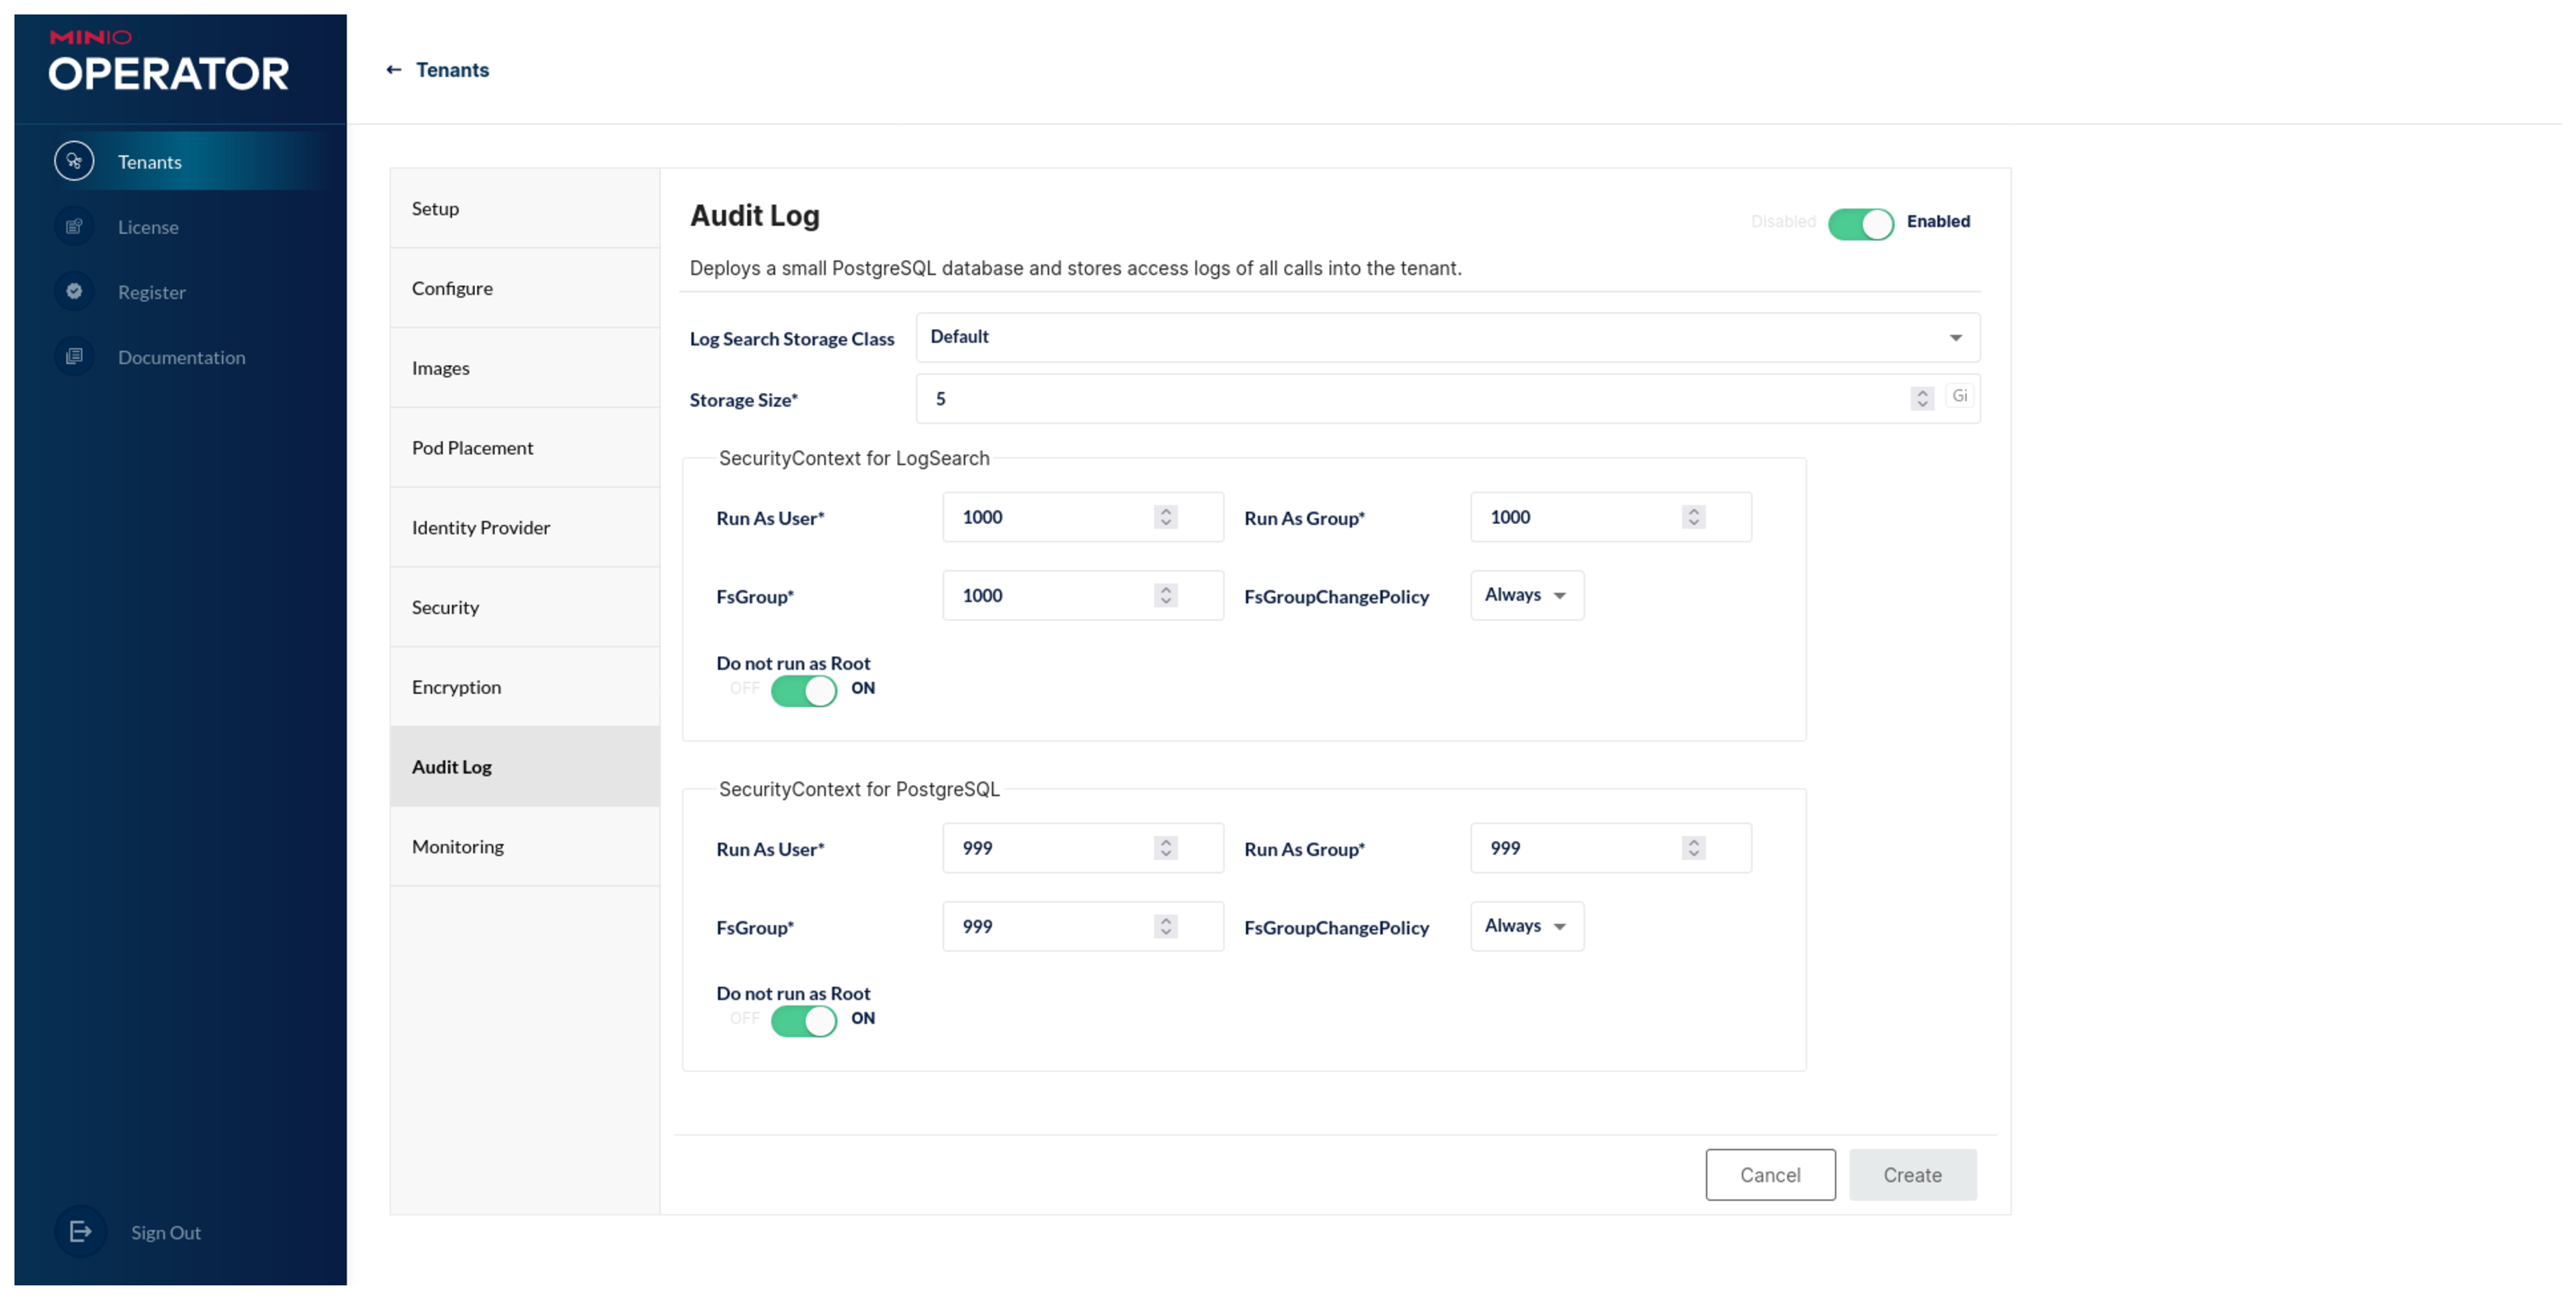
\includegraphics[angle=0, width=0.9\textwidth, height=0.9\textheight]{images/auditlog_minio.eps}
\end{center}
\end{figure}

\end{frame}

%%%%%%%%%%%%%%%%%%%%%%%%%%%%%%%%%%%%%%%%%%%%%%%%%%%%%%%%%%%%%%%%%%%%%%%%%%%%%%%%

\begin{frame}[fragile]{Création d'un tenant - Supervision - Minio}

\begin{figure}
\begin{center}
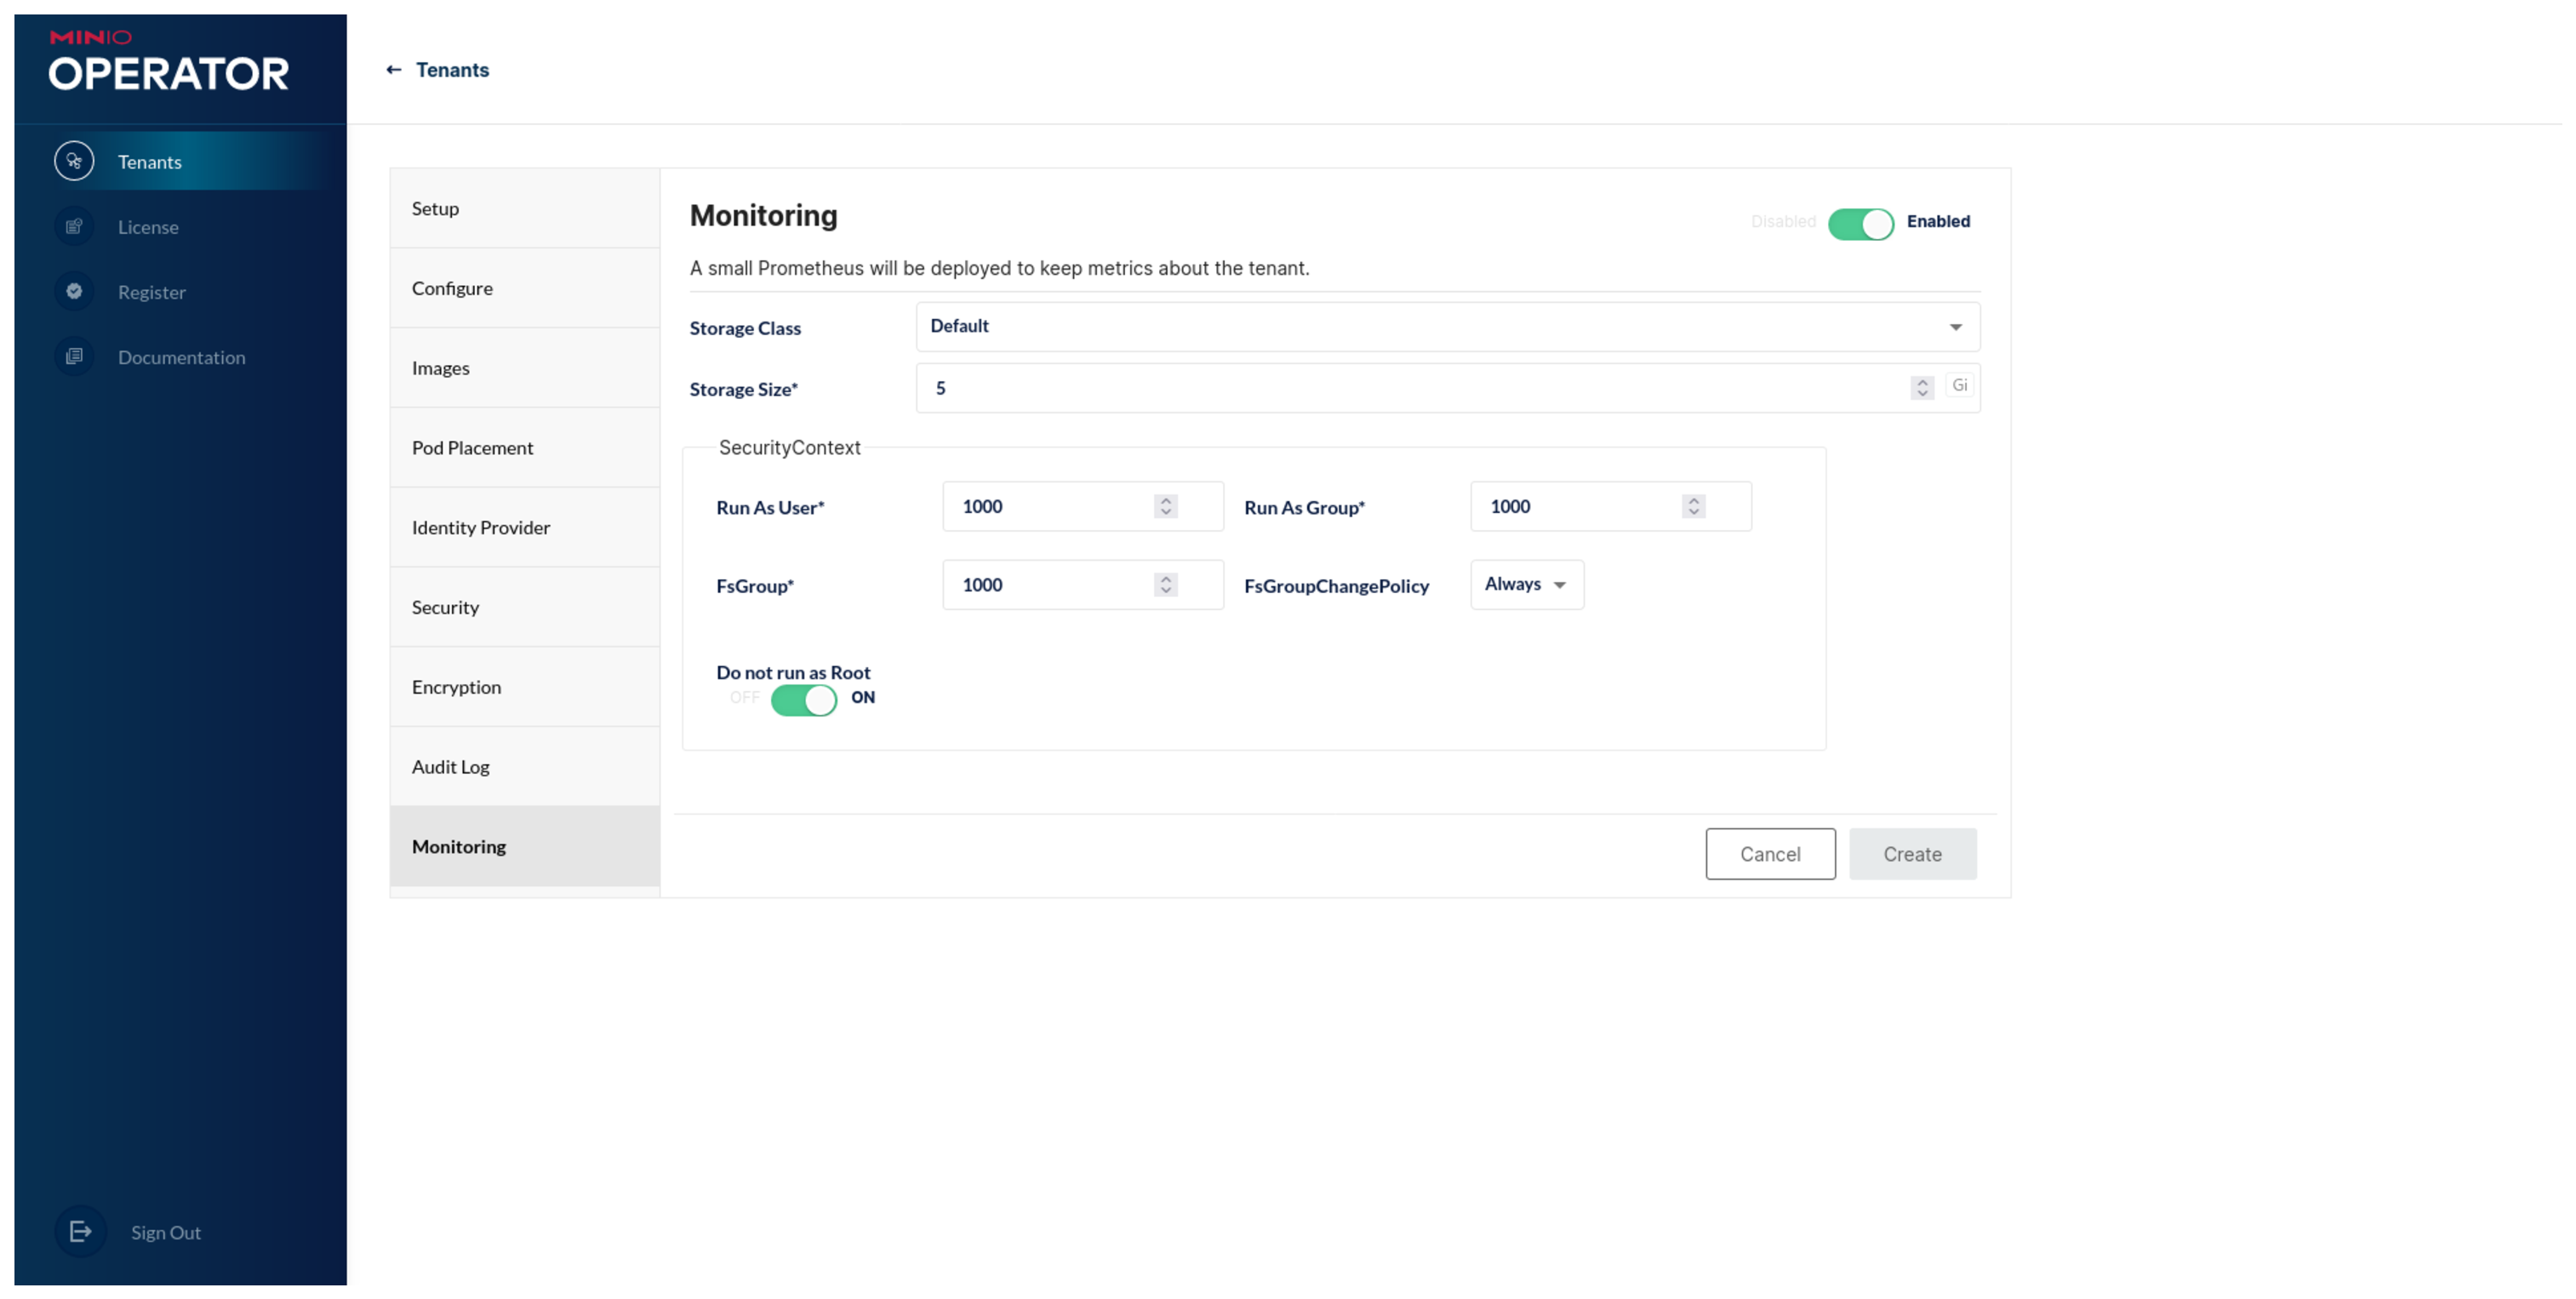
\includegraphics[angle=0, width=0.9\textwidth, height=0.9\textheight]{images/monitoring_minio.eps}
\end{center}
\end{figure}

\end{frame}

%%%%%%%%%%%%%%%%%%%%%%%%%%%%%%%%%%%%%%%%%%%%%%%%%%%%%%%%%%%%%%%%%%%%%%%%%%%%%%%%

\begin{frame}[fragile]{Clé d'accès et secret - Minio}

   WIP

\end{frame}

%%%%%%%%%%%%%%%%%%%%%%%%%%%%%%%%%%%%%%%%%%%%%%%%%%%%%%%%%%%%%%%%%%%%%%%%%%%%%%%%

\begin{frame}[fragile]{Image Docker utilisée par l'opérateur PostgreSQL}

   L'image déployée par l'opérateur PostgreSQL de Zalando s'appuie sur Spilo 
\url{https://github.com/zalando/spilo}

   Cette information se trouve dans le script \textbf{manifests/complete-postgres-manifest.yaml}:
\begin{Verbatim}[commandchars=\&\#\#]
  dockerImage: ghcr.io/zalando/spilo-15:3.0-p1
\end{Verbatim}

\end{frame}

%%%%%%%%%%%%%%%%%%%%%%%%%%%%%%%%%%%%%%%%%%%%%%%%%%%%%%%%%%%%%%%%%%%%%%%%%%%%%%%%

\begin{frame}[shrink=7,fragile]{Utilisation de container en mode rootless dans OpenShift}

   L'URL suivante décrit la problèmatique d'utilisation de container dans un environnement rootless: \\
   \begin{tiny}
   \url{https://docs.bitnami.com/tutorials/running-non-root-containers-on-openshift} \\
   \end{tiny}
   Cette page fournit également un lien intéressant sur la sécurisation d'un cluster Kubernetes en se basant sur les \textbf{Pod Security Policies}.\\
   Le lien est le suivant: \\
   \begin{tiny}
   \url{https://docs.bitnami.com/tutorials/secure-kubernetes-cluster-psp/}.
   \end{tiny}

\end{frame}

%%%%%%%%%%%%%%%%%%%%%%%%%%%%%%%%%%%%%%%%%%%%%%%%%%%%%%%%%%%%%%%%%%%%%%%%%%%%%%%%

\begin{frame}[fragile]{Pod Security Policies}

   Comme indiqué dans \url{https://kubernetes.io/docs/concepts/security/pod-security-policy/}, les PSP sont dépréciés.\\
   Ils sont maintenant remplacés par \textbf{Pod Security Admission} \url{https://kubernetes.io/docs/concepts/security/pod-security-admission/}.
   La norme \textit{Pod Security Admission} définit la notion de \textit{Security Context} décrite dans le lien suivant:
   \url{https://kubernetes.io/docs/tasks/configure-pod-container/security-context/}
   C'est cette notion qui va permet d'approcher au plus près les condictions de run d'un cluster Openshift 

\end{frame}

%%%%%%%%%%%%%%%%%%%%%%%%%%%%%%%%%%%%%%%%%%%%%%%%%%%%%%%%%%%%%%%%%%%%%%%%%%%%%%%%

\begin{frame}[fragile]{Opérateur - Security Context}

   Par défaut, l'opérateur PostgreSQL de Zalando applique les mesures de sécurité suivantes.\\
   Extrait de manifests/postgres-operator.yaml:

\begin{tiny}
\begin{Verbatim}[commandchars=\&\#\#]
securityContext:
    runAsUser: 1000
    runAsNonRoot: true
    readOnlyRootFilesystem: true
    allowPrivilegeEscalation: false
\end{Verbatim}
\end{tiny}

\begin{itemize}
   \item Il ne tourne pas avec un identifiant privilégié ni le compte root
   \item Il s'appuie sur des filesystems en lecture seule
\end{itemize}

\end{frame}

%%%%%%%%%%%%%%%%%%%%%%%%%%%%%%%%%%%%%%%%%%%%%%%%%%%%%%%%%%%%%%%%%%%%%%%%%%%%%%%%

\begin{frame}[fragile]{Pods PostgreSQL - Security Context}

   Il est possible d'affecter:
\begin{itemize}
   \item un utilisateur non privilégié
   \item un groupe non privilégié au pod.
   \item un groupe de filesystem défini
\end{itemize}

   Extrait de manifests/complete-postgres-manifest.yaml:
\begin{tiny}
\begin{Verbatim}[commandchars=\&\@\@]
  spiloRunAsUser: 101
  spiloRunAsGroup: 103
  spiloFSGroup: 103
\end{Verbatim}
\end{tiny}

\end{frame}

%%%%%%%%%%%%%%%%%%%%%%%%%%%%%%%%%%%%%%%%%%%%%%%%%%%%%%%%%%%%%%%%%%%%%%%%%%%%%%%%

\begin{frame}[fragile]{Installation d'ArgoCD}

Le lien suivant décrit l'installation d'ArgoCD: \url{https://argo-cd.readthedocs.io/en/stable/#quick-start}

\begin{tiny}
\begin{Verbatim}[commandchars=\&\#\#]
kubectl create namespace argocd
kubectl apply -n argocd -f https://raw.githubusercontent.com/argoproj/argo-cd/stable/manifests/install.yaml
\end{Verbatim}
\end{tiny}

\end{frame}

%%%%%%%%%%%%%%%%%%%%%%%%%%%%%%%%%%%%%%%%%%%%%%%%%%%%%%%%%%%%%%%%%%%%%%%%%%%%%%%%

\begin{frame}[fragile]{Installation de la CLI ArgoCD}

Le lien suivant décrit l'installation de la CLI ArgoCD: \url{https://argo-cd.readthedocs.io/en/stable/cli_installation/#download-with-curl}

\begin{tiny}
\begin{Verbatim}[commandchars=\&\#\#]
curl -sSL -o argocd-linux-amd64 https://github.com/argoproj/argo-cd/releases/latest/download/argocd-linux-amd64
sudo install -m 555 argocd-linux-amd64 /usr/local/bin/argocd
rm argocd-linux-amd64
\end{Verbatim}
\end{tiny}


\end{frame}

%%%%%%%%%%%%%%%%%%%%%%%%%%%%%%%%%%%%%%%%%%%%%%%%%%%%%%%%%%%%%%%%%%%%%%%%%%%%%%%%

\begin{frame}[fragile]{Activation de l'accès au serveur d'API d'ArgoCD}

Le lien suivant décrit les différentes méthodes d'accès au serveur d'API d'ArgoCD: \url{https://argo-cd.readthedocs.io/en/stable/getting_started/#3-access-the-argo-cd-api-server}

\begin{tiny}
\begin{Verbatim}[commandchars=\&\#\#]
$ kubectl patch svc argocd-server -n argocd -p '{"spec": {"type": "LoadBalancer"}}'
service/argocd-server patched
\end{Verbatim}
\end{tiny}

\end{frame}

%%%%%%%%%%%%%%%%%%%%%%%%%%%%%%%%%%%%%%%%%%%%%%%%%%%%%%%%%%%%%%%%%%%%%%%%%%%%%%%%

\begin{frame}[fragile]{Build de l'image Docker Spilo}

   Le Dockerfile définissant l'image Spilo est disponible à l'URL suivante: \url{https://github.com/zalando/spilo} \\

   La méthode de génération de l'image est décrite dans: \url{https://github.com/zalando/spilo#how-to-build-this-docker-image} \\

\begin{tiny}
\begin{Verbatim}[commandchars=\\\#\#]
$:~/spilo/postgres-appliance$ docker build --tag dnum-test .                                                                                                            
[+] Building 9762.1s (33/33) FINISHED                                                                                                                                                         
 => [internal] load build definition from Dockerfile                                                                                                                                     5.8s 
 => => transferring dockerfile: 3.01kB                                                                                                                                                   0.0s 
 => [internal] load .dockerignore                                                                                                                                                        6.9s
 => => transferring context: 2B                                                                                                                                                          0.0s
\ldots
 => => exporting layers                                                                                                                                                                154.5s 
 => => writing image sha256:52afd69aff9414333220ec408283a8ff20e2162e703c6ab5afd5090d9d62e4e0                                                                                             1.0s
 => => naming to docker.io/library/dnum-test                                                                                                                                             1.1s

\end{Verbatim}
\end{tiny}

   Le build dure un peu moins de \textbf{2h43min}.
\end{frame}

%%%%%%%%%%%%%%%%%%%%%%%%%%%%%%%%%%%%%%%%%%%%%%%%%%%%%%%%%%%%%%%%%%%%%%%%%%%%%%%%

\begin{frame}[fragile]{Login avec la CLI d'ArgoCD}
La commande suivante permet de récupérer le mot de passe initial de l'admin d'ArgoCD:

\begin{tiny}
\begin{Verbatim}[commandchars=\\\#\#]
linagora@debian-cp:~$ argocd admin initial-password -n argocd
*******************

 This password must be only used for first time login. We strongly recommend you update the password using `argocd account update-password`.
\end{Verbatim}
\end{tiny}

\end{frame}

%%%%%%%%%%%%%%%%%%%%%%%%%%%%%%%%%%%%%%%%%%%%%%%%%%%%%%%%%%%%%%%%%%%%%%%%%%%%%%%%

\begin{frame}[fragile]{Login avec la CLI d'ArgoCD}

\begin{tiny}
\begin{Verbatim}[commandchars=\\\{\}]
$ kubectl get svc -n argocd
NAME                                      TYPE           CLUSTER-IP       EXTERNAL-IP   PORT(S)                      AGE
argocd-applicationset-controller          ClusterIP      10.109.27.242    <none>        7000/TCP,8080/TCP            6d16h
argocd-dex-server                         ClusterIP      10.100.63.110    <none>        5556/TCP,5557/TCP,5558/TCP   6d16h
argocd-metrics                            ClusterIP      10.102.19.237    <none>        8082/TCP                     6d16h
argocd-notifications-controller-metrics   ClusterIP      10.102.70.229    <none>        9001/TCP                     6d16h
argocd-redis                              ClusterIP      10.104.253.209   <none>        6379/TCP                     6d16h
argocd-repo-server                        ClusterIP      10.111.28.234    <none>        8081/TCP,8084/TCP            6d16h
\textbf{argocd-server                             LoadBalancer   10.109.47.144    <pending>     80:30235/TCP,443:30885/TCP   6d16h}
argocd-server-metrics                     ClusterIP      10.98.167.31     <none>        8083/TCP                     6d16h
linagora@debian-cp:~$ argocd login 10.109.47.144
WARNING: server certificate had error: x509: cannot validate certificate for 10.109.47.144 because it doesn't contain any IP SANs. Proceed insecurely (y/n)? y
Username: admin
Password: 
'admin:login' logged in successfully
Context '10.109.47.144' updated

\end{Verbatim}
\end{tiny}

\end{frame}

%%%%%%%%%%%%%%%%%%%%%%%%%%%%%%%%%%%%%%%%%%%%%%%%%%%%%%%%%%%%%%%%%%%%%%%%%%%%%%%%

\begin{frame}[fragile]{Guestbook - ArgoCD}

   ArgoCD s'appuie sur un \textit{guestbook} pour piloter un déploiement dans un cluster k8s.
   Un exemple de guestbook est disponible à l'URL suivante: \url{https://github.com/argoproj/argocd-example-apps.git}

\end{frame}

%%%%%%%%%%%%%%%%%%%%%%%%%%%%%%%%%%%%%%%%%%%%%%%%%%%%%%%%%%%%%%%%%%%%%%%%%%%%%%%%

\begin{frame}[fragile]{Intégration avec ArgoCD}

   WIP

\end{frame}

%%%%%%%%%%%%%%%%%%%%%%%%%%%%%%%%%%%%%%%%%%%%%%%%%%%%%%%%%%%%%%%%%%%%%%%%%%%%%%%%

\begin{frame}[fragile]{Accès client à la base de données}

   WIP

\end{frame}

%%%%%%%%%%%%%%%%%%%%%%%%%%%%%%%%%%%%%%%%%%%%%%%%%%%%%%%%%%%%%%%%%%%%%%%%%%%%%%%%

\begin{frame}[fragile]{Point-in-time recovery PITR}

   WIP

\end{frame}

%%%%%%%%%%%%%%%%%%%%%%%%%%%%%%%%%%%%%%%%%%%%%%%%%%%%%%%%%%%%%%%%%%%%%%%%%%%%%%%%

\begin{frame}[fragile]{Failover - Changement du nombre de pods}

   WIP

\end{frame}

%%%%%%%%%%%%%%%%%%%%%%%%%%%%%%%%%%%%%%%%%%%%%%%%%%%%%%%%%%%%%%%%%%%%%%%%%%%%%%%%

\begin{frame}[fragile]{Mise à jour mineure de PostgreSQL}

   WIP

\end{frame}

%%%%%%%%%%%%%%%%%%%%%%%%%%%%%%%%%%%%%%%%%%%%%%%%%%%%%%%%%%%%%%%%%%%%%%%%%%%%%%%%

\begin{frame}[fragile]{Mise à jour majeure de PostgreSQL}

   WIP

\end{frame}

%%%%%%%%%%%%%%%%%%%%%%%%%%%%%%%%%%%%%%%%%%%%%%%%%%%%%%%%%%%%%%%%%%%%%%%%%%%%%%%%
